\documentclass[b5paper,twoside,openright,11pt]{report}
\usepackage[printonlyused]{acronym}
\usepackage{graphicx}
\usepackage{enumerate}
\usepackage{cite}
\usepackage{float}
\usepackage[utf8]{inputenc}
\usepackage[hyphens]{url}
\usepackage{rotating}
\usepackage{array}
\usepackage{amsmath}
\usepackage{fancyhdr}
\usepackage[parfill]{parskip}
\setlength{\headheight}{25.23pt}
\renewcommand{\headrulewidth}{0pt}
\pagenumbering{gobble}
\begin{document}
\begin{flushleft}
\begin{figure}[htb]

\includegraphics[scale=0.6]{NTNU-logo}
\end{figure}
\bigskip
\bigskip
\bigskip
\bigskip
\begin{huge}
\textbf{Masteroppgave}\\
\end{huge} 
\bigskip
\bigskip
\bigskip
\bigskip
\bigskip
\bigskip
\bigskip
\begin{Large}
\textbf{Kine Aa. Omholt and Mathilde Wærstad \\}
\end{Large}
\bigskip
\bigskip
\bigskip
\bigskip
\bigskip
\bigskip
\begin{large}
\textbf{Master Thesis\\}
\end{large}
Delivered: \today\\
Professor: Lill Kristiansen\\
Supervisor: Ather Nawaz\\
\bigskip
\bigskip
\bigskip
\bigskip
\bigskip
Norwegian University of Science and Technology\\ 
Faculty of Information Technology, Mathematics and Electrical Engineering\\
Department of Telematics
\end{flushleft}
\cleardoublepage
\begin{abstract}

\end{abstract}
\cleardoublepage
\chapter*{Preface}
This thesis is written as a part of our master's degree in Communication Technology, with focus in Tele-economics, at the Norwegian University of Science and Technology (NTNU). The focus of this thesis has been to design a video game concept for elderly, and it is a continuation of work done in our project assignment. 

We would like to thank our professor Lill Kristiansen for valuable guidance and feedback on our work during this final semester. The result of this thesis would not have been the same without her ideas and comments. We would also like to thank supervisor Ather Nawaz for stepping in when we needed him the most. His help has been highly appreciated the few final weeks before handing in the master thesis.  

"Seniornett" deserve a great thank you for their contribution to our assignment. This, especially, yields Arne Sølvberg, the manager of "Seniornett" in Trondheim. He has helped us a lot with arrangement of meeting, booking of facilities, moving needed equipment, and engaging elderly to join our workshops. We would not have been able to perform these workshops without his help. We are also grateful to the eight seniors from "Serniornett" who had time and willingness to participate in our workshops. Their feedback and opinions have been used as part of the basis for our master thesis. We would also thank Pål Sæther from the Department of Telematics for always helping us finding the equipment we would need.        

Finally, we would thank our families for all the support we have got during all our time as students. We are forever grateful! And to all our classmates and friends, thank you for all the fun and good memories! The time here at NTNU has been unforgettable. And to each other, a thank you for a great semester. We finally made it!   

\cleardoublepage
\pagenumbering{roman}
\tableofcontents
\cleardoublepage
\chapter*{Acronyms}
\begin{acronym}
\acro{nsd}[NSD]{Norsk Samfunnsvitenskapelig Datatjeneste}
\acro{usid}[USID]{User Sensitive Inclusive Design}
\acro{ucd}[UCD]{User Centered Design}
\acro{d3}[D3]{Design for Dynamic Diversity}
\acro{dtc}[DTC]{Dual Task Costs}
\end{acronym}
\cleardoublepage
\listoffigures
\cleardoublepage
\listoftables
\cleardoublepage
\pagenumbering{arabic}
\pagestyle{fancy}
\fancyhead[LE]{\thepage}
\fancyhead[RE]{\leftmark}
\fancyhead[RO]{\thepage}
\fancyhead[LO]{\rightmark}
\fancyfoot{}
\chapter*{Descriptions}
Usability \\
Heuristics \\ 
Exergames \\
Kinect \\ 
Workshop \\

\cleardoublepage
\chapter{Introduction}
\section{Contribution}
\section{Scope and Limitation}
\section{Outline}
\cleardoublepage
\chapter{Background}
\section{Video Games}
Video games are a genre of digital games that has become extremely popular all over the world. There exist several different gaming consoles, and for each console there has been developed an endless amount of different games that meets almost every need and interest. Video games can be described as “electronic, interactive games known for their vibrant colors, sound effects, and complex graphics” \cite{videogamedef}. Hand held controllers or devices that capture movement are used to interact with the video game. The variety of video games makes it usable for many different purposes, like learning and education, exercising or just pure entertainment (veldig likt som oppgaven) \cite{project}. \\ \\
One might associate video games with children and teenagers, and many hours of game play, which partly is a right assumption to make. Video games are played for several hours every day, and it has taken a great part in people's everyday life. Gaming was usually associated with being anti-social, because of all the time used looked up in a room playing, but video games has emerged from sedentary, lonely gaming to gaming involving social interaction and movement. In USA in 2010, one fourth of all gamers were under the age of 18, but an interesting fact is that as much as 26 percent of the gamers are over 50 years old. This shows that not only children and teenagers uses video games, a great share of elderly has started to use this type of technology. In Norway,  as much as 8 percent of the population in the age range from 45 - 79 use computer or video games every day \cite{project}. Elderly contributes to a great share of the world's population, and if the entertainment industry could see this group as potential customers, it would open up a new and inexperienced market for video games \cite{ijsselsteijn2007digital}. 
\section{Serious Video Games}
The widespread and assorted use of video games has made a great potential for the entertainment industry with regard to development of new games, but also in terms of developing games for additional purposes beside pure entertainment. A new way to use video games is for 
different types of training, education and learning, which is called serious games. Serious games can be described as “a mental contest, played with a computer in accordance with specific rules, that uses entertainment to further government or corporate training, education, health, public policy, and strategic communication objectives.” [fra From Visual Simulation to Virtual Reality to Games] The idea is to use the fun, motivating and captivating features that video games possess and combine it with pedagogy. The term serious games is not something new, it has existed for many years, but it did not break through when it first was introduced in the 1990s. The failure that time was that the focus of the game was on learning, which resulted in boring games with no market success \cite{susi2007serious}. Michael Zyda states that, in serious games, pedagogy has to be subordinate (SAMME ord som i teksten) to the story and entertainment component of the game. It is important that fun and entertainment are the main focus in the game \cite{zyda2005visual}. \\ \\
There exist several genres of serious games, where game-based learning, simulation games, games with a purpose, games for health and exergames are some of them. How and where serious games can be used, and are being used today, are many. With simulation games medical students can simulate surgery and soldiers can practise on how to use a rifle, students can learn their curriculum through quiz games, and people can be motivated to work out with exercise games. Research on use of serious games shows positive evolvement of skills and knowledge, and positive effect on health, which results in motivation for further research and development. (VET ikke om dette er rett ord å bruke). In addition, the new technology involving physical interfaces and improvement on graphics and animations initiates to new types of games. The market for serious games are inexperienced and unexplored, so there are a great potential for further research \cite{alfingewang}. Market sales the last couple of years also shows promise for serious games in the future. In 2008, the market for serious games sold for around 1,5 billion USD around the globe \cite{alfingewang}, and in 2010 it reached about 2 billion USD (1,5 billion EUR). The market is expecting a annual growth rate of 47 percent, up to about 13,5 billion USD (10 billion EUR) in 2015! \cite{idate} \\ \\
We will look deeper into one of the genres of serious games, exergames.  
\section{Exergames}
Skrive et kort sammendrag av hva exergames er og hvordan det blir brukt i dag. Ramse opp kjapt hva som går under exergames. 
\section{Exergames Used in Rehabilitation and Exercising}
Relevant arbeid der det er bevist at spill kan brukes for trening for eldre.. 
\section{Microsoft Kinect}
Beskrive Kinect nærmere og også grunnen til valget av Kinect. 
\section{How to Develop a Good Video Game?}
Related work.. Generelt om hva som skal til for å utvikler videospill. Dra noen konklusjoner.
\section{How to Develop a Good Exergame for Elderly}
Related work der de snakker om alle de viktige tingene vi må tenke på når man utvikelr for eldre..


\cleardoublepage
\chapter{Barriers and Motivation to Exercise in Elderly People  }
\label{chap:olderexercise}

An exergame for elderly needs to include the right exercises, as well as motivating elements, to engage the user group to use it. Meeting this, we have to understand what motivates elderly to exercise in general. There are different challenges and barriers that keep older people from exercising, and it is shown that only a small share of elderly meets official requirements of physical activity. There exist various proposed guidelines on how elderly people should exercise, and there are different services that both can be implemented at home, and performed outside the home. Introducing an exergame, which integrates already existing exercises in a story with focus on entertainment, can be a fun, motivating and effective alternative to existing services.  

In Section \ref{sec:exercisebehaviour} we will discuss older people's attitude towards exercising, and look at numbers that support the need for an alternative way to exercise. Guidelines on how elderly should exercise will briefly be discussed, but the interested reader are referred the original references for more information, as this is out of our area of competence. In Section \ref{sec:barriers} we will discuss typical barriers and challenges that keep elderly from exercising. At last, in Section \ref{sec:motivators} we will discuss motivating factors that will be taken into account in the development of the game concept.  

\section{Elderly and Exercising}
\label{sec:exercisebehaviour}
Physical activity is important for all people, including elderly. It can improve quality of life by reducing risk of some chronic diseases, alleviate depression, and help people towards a more independent life. Improving health by physical activity does not just apply for healthy elderly, but also for frail and very old people. Guidelines are proposed by different entities, like The Norwegian Directorate of Health and the U.S. Department of Health and Human Services, recommending physical activities like aerobic activity, as well as strengthening exercises \cite{aktivitetsbok} \cite{guidelines}. A set of guidelines for how to exercise may seem easy to follow, but it is shown to be challenging to motivate elderly to exercise. There is shown that there is only a small percentage of elderly who actually engage in physical activity \cite{olderamericans}. To be able to engage seniors to be more physically active, they should be provided with programs that will motivate them to actually perform the exercises. In this thesis, we will develop a exergame concept for this purpose. As discussed in our previous project \cite{project}, keeping the older population healthy can, in addition to decrease the risk of falling, reduce the need for health services, and also decrease economic challenges related to this. It is therefore important to have focus on the older populations' physical health. 

Norwegian elderly, aged  67-79 years old, have become more active the last years, with as much as 40 percent of this population exercising regularly several times a week \cite{statisticsnorway}. However, only one fifth of adults meet the minimum requirements recommended by The Norwegian Directorate of Health, which is 30 minutes of exercising per day \cite{statistikknorge12}. 23 percent of the group between 67-79 years old in Norway exercise less than once a month or never \cite{statisticsnorway}, which states that there are many adults that do not meet these requirements. It is shown that some exercise is better than none, and they should therefore be engaged in physical activity. Even though exercise once a week not is enough, it have some positive effects on elderly \cite{gruppetrening-trheim}. The numbers are worse in other parts of the world. The Federal Interagency Forum on Aging Related Statistics \cite{olderamericans} presented numbers in their latest report, revealing that only 11 percent of Americans aged 65 years and older, meet the 2008 Federal Physical Activity Guidelines \cite{guidelines}. The percentage decrease with increasing age, where 14 percent of older people aged 65-74 years old meet these guidelines, while this is the case for only 4 percent of people over the age of 85. It is quite common that physical activity decrease with age and that after the age of 65 years old, the level of activity is at its lowest \cite{schutzer}. 
 
The Norwegian Directorate of Health has made a handbook for physical activity for prevention and treatment. They recommend that regular activity that includes the major muscle groups should be performed 2-3 days a week, 20 minutes each time. Different activities suggested includes cycling, swimming, walking, jogging and cross-country skiing. Activities that involves resistance training has shown positive effect also for elderly people. It is recommended that exercises that include all main muscle groups should be performed 1-2 times a week, be done for 10-12 repetitions, and be progressive. In addition, it is recommended to perform exercises that will strengthen mobility, gait and balance function. Exercises for improving balance, should be customised for each individual's needs. Mobility is best maintained by regularly moving the body, both with everyday movements and physical activity. Exercises that have proved good for improving balance functions include stand on one foot, or walk in circles, sideways, or over obstacles. In addition, a regular walk in various terrain is a good and convenient activity to maintain balance function, gait and mobility \cite{aktivitetsbok}. The readers interested in the specific guidelines proposed by The Norwegian Directorate of Health and the U.S. Department of Health and Human Services will be referred to  \cite{aktivitetsbok} and \cite{guidelines}. 

In our previous project \cite{project} we presented different training programs that are made especially for elderly. One of these are "Øvelsesbanken", which is created by the physiotherapy service in Trondheim, Norway.  "Øvelsesbanken" is a service primarily meant for physiotherapists to in an convenient way put together exercise programs for their patients to perform at home. However, private users have the possibility to register, and put up their own programs, as well. The main purpose with the exercises is fall prevention, and includes exercises to increase balance and strength \cite{eldretrening}. We found these exercises relevant for the exergame. We have chosen to build the concept around these exercises, together with the activities proposed by The Norwegian Directorate of Health. This will give us a set of exercises shown to be good for elderly, that we could not have put together ourselves, as we do not have the competence to recommend exercises.

Age-related physically and mentally changes can be reduced with regular physical activity. There exist several guidelines on how and what to exercise, however, there are various challenges when it comes to motivating elderly people to exercise. These will be discussed in the next section. 

\section{Barriers and Challenges}
\label{sec:barriers}
It is hard to get people to be physical active, and this might especially apply for elderly. Because of the high fall statistics there is important to engage elderly in physical activity, as the main reason for falls are reduced physical strength and decreased balance. General guidelines suggest that elderly should perform exercising programs that contains exercises that strengthen muscles, balance, endurance and mobility \cite{gruppetrening-trheim}. There are some unique challenges and barriers when it comes to engaging elderly in physical activities discussed in the literature. Understanding these barriers will make it easier to identify how to motivate them to exercise. It is crucial when developing exercise programs, to understanding the motivational factors behind exercising \cite{chao}.

One common barrier is that elderly think their health is not good enough to start exercising \cite{schutzer}, and may believe exercising will do more harm than good \cite{chao}. Their poor health and the pain related to this, hinders them from exercising. In addition, elderly have a tendency of thinking they are too old to start exercising \cite{schutzer}. A significant challenge is to get people to exercise long enough to see positive results. Many associate exercising with pain, sweating, and muscle soreness, and the time before positive outcomes are noticed can be long. At the same time, the negative effects of not exercising, may not be that apparent \cite{chao}. 

The importance of having available and convenient resources is significant, as it is shown that people living far away from training centres, parks and walking paths are less active than people living near these facilities \cite{schutzer}. With this comes also time constraints. It is shown that many elderly look at physical activity as time consuming, thinking about the time doing the activity, as well as the time getting to the exercise site \cite{schutzer} \cite{chao}. It can be challenging to get people to perform unstructured, free-living, exercise programs, compared to structured programs. This is because people themselves have to decide when, where, and what to do. This is pretty much based on self-motivation \cite{chao}.  

Physicians play an important role when it comes to advising elderly to exercise, because most people have respect for and trust their physicians. This was also discussed in \cite{project}, where we found physiotherapists to be an appropriate and reliable mediator for the exercise game. However, in \cite{schutzer} and \cite{chao}, it is discussed that physicians do not always give sufficient exercise advice. Instead of giving a specific exercise program for the patient to perform, they simply just tell them to be more active. Many elderly have little knowledge about physical activity and its advantages. This can come from the fact that many elderly grew up in a time where people generally were more active in their everyday life, and where there were not that much attention around the importance of physical activity \cite{schutzer}. In addition, many think of physical activity more as a recreation activity, or something people do for competition, and are not looked as necessary for keeping a good health.  

\section{Strategies and Motivators}
\label{sec:motivators}
Understanding barriers and challenges give an understanding on what factors that motivate people to exercise. Having more time, more information, and living closer to exercise offerings, are basic goals that can serve as good motivators for exercise. Chao et al. \cite{chao} propose that a structured program offered at a set time, probably will be a good solution for this user group, as a common problem is to find time, as well as decide which exercises to do. A strategy is to focus on what physicians are telling their patients. It is important to remember the common limitation of memory capacity among elderly. Therefore, information should be given in a precise and accurate way \cite{chao}.  

Chao et al. discuss strategies for motivation \cite{chao}. One must understand different peoples' needs and expectations, and take into account race, gender, ethnicity etc. To meet these expectations, contact with the relevant people is important. The researchers suggest this to be done with for example interviews and focus groups \cite{chao}. Self-regulatory skills, including goal setting, self-monitoring of progress, and environmental management, are important to keep peoples' exercise behaviour \cite{chao}, \cite{schutzer}. The feeling of pleasure and satisfaction are also important \cite{schutzer}.  Clear goals should be set to let the participant understand that the activity has a purpose and is going through an end, and that skills will be developed through practice. To easily monitor the exercise, goals should be separated into small and more manageable parts. Implementing decision-making models, modifying cognitive thoughts during activity, and increasing social support are also strategies to promote adherence to physical activity \cite{chao}.  Exercising should be looked at as an ongoing process, and it is important to remember that people's behaviour towards exercising can change with age. Therefore, prevention of relapse should be included in the planning process, to maintain physical activity routines \cite{chao}. 

Self-efficacy seems to be an important determinant for exercise behaviour. Self-efficacy is defined in \cite{schutzer} as \emph{"an individuals belief in their ability to successfully perform a specific behaviour"}, and it is said that it is more likely for a person with strong self-efficacy expectations and outcomes to adopt to a specific behaviour. In \cite{white} they evaluate self-efficacy to play an important role in the relationship between physical activity and quality of life. White et al. did a study where they measured a sample of community dwelling adults' physical activity, self-efficacy, global quality of life, physical self worth, and disability limitations. They concluded that \emph{"being more active was associated with being more efficacious, having fewer disabilities limitations, reporting higher physical self-worth, and being more satisfied with one's life"} \cite{white}. In addition, \cite{white} stated that self-esteem is an important component of the physical activity and quality of life relationship. 

Schutzer et al. suggest some alternative motivating factors \cite{schutzer} which can help preventing relapse. They suggest prompts, like e-mail and telephone contact. These prompts are typically used for home based training programs, and are shown to be at least as effective as supervision face-to-face. Telephone contact works well in a starting phase, when trying to get a person to adopt to a more active lifestyle, while e-mail contact works well to help maintain this lifestyle. These ways can actually be more effective than prolonged exercise session with face-to-face contact \cite{schutzer}. For home based training programs, telephone contact is seen as valuable for encouraging, reward and monitor the person's progress \cite{chao}.  

The last important motivator discussed in \cite{schutzer} is appropriate music to enhance the exercise experience, and to divert from pain coming from the exercises. 


\subsection{Summary of motivator factors for exercising}
\label{subsec:motivator}

From the literature presented in this chapter we have drawn out 13 motivational factor for exercise behaviour. These are listed below, and will be taken into consideration when specifying requirements for our exergame concept. 

\begin{enumerate}[{m}.1]
\item Convenience of activity facilities \cite{chao}, \cite{schutzer}
\item Precise information about what to exercise \cite{chao}, \cite{schutzer}
\item Sufficient information about the benefits of exercising \cite{chao}, \cite{schutzer}
\item Self-efficacy and self-esteem \cite{schutzer}, \cite{white}
\item Self-regulatory skills \cite{chao}, \cite{schutzer}
\item Small and manageable goals \cite{chao},\cite{schutzer}
\item Self-monitoring of progress \cite{chao},\cite{schutzer}
\item Modifying cognitive thoughts \cite{chao}
\item Decision making \cite{chao}
\item Social support \cite{chao}
\item Meet different peoples' needs and expectations \cite{chao}
\item Prompts, either face-to-face, by telephone or e-mail \cite{chao},\cite{schutzer}
\item Appropriate music \cite{schutzer}
\end{enumerate} 

\bigskip

When designing physical training programs, understanding the factors that motivate people to exercise is very important. The motivational factors discussed in this chapter will be considered when we develop an exergame concept for elderly. In addition different activities presented by The Norwegian Directorate of Health as well as the exercises presented in "Øvelsesbanken" will be considered. There are additional factors that needs to be studied that are more related to video games and elderly. This will be looked into in Chapter \ref{chap:exforseniors} and \ref{sec:designelderly}. First we will briefly present what video games are, and how they can be used for exercising. 





\cleardoublepage
\chapter{Exercise Games}
In this chapter we will present what exercise games are and how it can be used for exercising. To understand the concept of exergames and where it originates from, we will start with a brief presentation of what video games and serious games are. We will also present the technology that will be used for the game we are developing a concept for, namely Microsoft Kinect. 

\section{Video Games}

Video games are a genre within digital games that has become extremely popular all over the world. There exist several different gaming consoles, and for each console there has been developed an endless amount of various games that meets almost every need and interest. Video games can be described as \emph{"electronic, interactive games known for their vibrant colors, sound effects, and complex graphics"} \cite{videogamedef}. Hand held controllers or devices that capture movement are used to interact with the video game. The variety of video games makes it usable for many different purposes, like learning, education, physical activity, or just for the sake of amusement \cite{project}. 

One might associate video games with children and teenagers, and many hours of game play. Generally, this is a right assumption to make. In USA, video games are played for several hours every day \cite{foxnews}, and one third of all gamers are under the age of 18 \cite{videogames2012}. Gaming are usually associated with being anti-social, because of all the time spent looked up alone in a room, playing. However, the gaming lifestyle have changed. Video games has emerged from sedentary, lonely gaming, to gaming involving social interaction and movement, and it has taken a great part in people's everyday life. In Norway, 6 percent of the population in the age range 45 - 79 use computer or video games every day \cite{mediebarometer2012}. This might indicate that not only children and teenagers uses video games, but also the elderly population have started to use this type of technology. Statistics from USA in 2011 provided numbers that might support this assumption, as they showed that as much as 29 percent of all gamers where over the age of 50 \cite{videogames2011}. Elderly contributes to a great share of the world's population, and if the entertainment industry could see this group as potential customers, it would open up a new and inexperienced market for video games \cite{ijsselsteijn2007digital}. 

\section{Serious Games}
\label{sec:sergames}
The widespread and assorted use of video games have made a great potential for the entertainment industry regarding development of new games, and also in terms of developing games for additional purposes beside pure entertainment. A new way to use video games is to include it in training, education and learning. This is called serious games. Serious games can be described as \emph{"a mental contest, played with a computer in accordance with specific rules, that uses entertainment to further government or corporate training, education, health, public policy, and strategic communication objectives"} \cite{zyda2005visual}. The idea is to use the fun, motivating and captivating features that video games possess and combine it with pedagogy. If a video game can be defined as a serious game depends on how the game is used, the purpose of the game and the users gaming experience. 

The first serious attempt in developing video games with the main focus on learning did not become very successful \cite{understandingvg}. The failure that time was that the focus in these  video games were on pure learning, which resulted in boring games that did not create motivation and curiosity \cite{understandingvg} \cite{susi2007serious}. Michael Zyda states that, in serious games, pedagogy has to be subordinate to the story and entertainment component of the game. It is highly important that fun and amusement is the main focus in the game \cite{zyda2005visual}. For a video game to function as a pedagogical tool it has to focus on motivation, effectiveness, debriefing, and intuitiveness. These games have to provide motivating factors that engage people to play the game, and they have to be effective in the matter of learning outcome. Debriefing has the intention of creating a state of mind where thoughts and feelings are processed after playing the game, and when it comes to intuitiveness, people have to be able to play and understand the video games without the need for guidance \cite{understandingvg}. 

There exist several genres of serious games, where edutainment and game-based learning, advertaintment, games for politics, simulation games, and games for health are some of them. The genre of edutainment and game-based learning combines fun and entertainment with education and learning. Advertainment is about using video games as a media for marketing, and games for politics influences players through hidden, underlying political messages in the game. Simulation games are about bringing various activities into life with the use of video games, and gaming for health is about using video games to engage activity, to become physically stronger, and to improve quality of life. Gaming for health includes a topic called exercise games, which has training as a main focus \cite{understandingvg} \cite{alfingewang}.

An important feature with serious games is that they provide the opportunity to experience real-life situations and adventures one may otherwise not be able to enjoy. This might be due to expenses, time, distance, risk, or physical capabilities. With serious games it is possible to play golf, be the star of a boxing match, paddle down turbulent rivers, and explore nature and creatures one have never seen before. In a more serious matter, video games can be used to simulate brain surgery or a battle in a war zone. This can teach students how to perform medical procedures or it could prepare soldiers for war. Serious games can also be used for students to learn their curriculum through quiz games, and people can be motivated to work out with exercise games. Serious games can be used for several purposes and situations, and it can help people develop a wide range of different skills. 

Research on the use of serious games show positive development of skills and knowledge, in addition to positive effect on health, which have resulted in motivation for further research and development. In addition, the new technology involving physical interfaces and improvement on graphics and animations initiates to new types of games. The market for serious games are inexperienced and unexplored, so there are a great potential for further research \cite{alfingewang}. Market sales the last couple of years also shows promise for serious video games in the future. In 2008, the market for serious games sold for around 1,5 billion USD around the globe \cite{alfingewang}, and in 2010 it reached about 2 billion USD (1,5 billion EUR). The market is expecting a annual growth rate of 47 percent, up to impressive 13,5 billion USD (10 billion EUR) in 2015 \cite{idate}. 

We will look closer into one of the genres within serious games, exercise games.  

\section{Exergames}
\label{sec:exergames}
Exergames are a type of serious video games that combine traditional game play with physical activity. The combination of movement and amusement is used to stimulate exercise and engage people to be more physically active in a fun and motivating way. A lot of research have been done within this topic, and results show that exergames can have a positive effect on users health. In addition to being a new, and more amusing way to work out, exergames provide an opportunity for social interaction. A great amount of today's existing computer and video games possess this feature, and as much as 62 percent of all gamers say they play with others either in-person or online. One of the two top-selling video games in 2011 was Just Dance 3, which is an exergame that has the possibility to play with others \cite{statistics2012}. This shows that the social aspect of gaming is important. The social aspect these games provide may also be especially important for people who experience loneliness in their everyday life \cite{exergamesforelderly}.

Exergames use technology like remote hand held controllers and motion sensors to capture body movements. Users are therefore required to get up and move their body to be able to play the game. There exist several consoles that support this technology, where Nintendo Wii, Playstation Move, Dance Dance Revolution and Xbox Kinect are some of them. The existing consoles use different type of devices to capture body movement, like hand held controllers, different boards and pads with embedded sensors, and video cameras with motion sensors. In this assignment we will focus on the Kinect sensor technology. This is because we in our previous project evaluated Kinect to be an appropriate choice as it provides the possibility to play without holding on to any devices, and because the sensor has proved to measure different body movements accurately so that the parameters are applicable for use in clinical practice. The reader will be referred to our project assignment \cite{project} and Section 4.2 to read what this is based on. We will now provide a brief description of the chosen technology.

\section{Microsoft Kinect for Xbox 360 and Windows}
Microsoft Kinect is a motion sensor that captures movement without the use of any controllers. This gives players the opportunity to play and interact with the game only by gestures and body movement. Xbox presents the Kinect experience this way: \emph{"Kinect for Xbox 360 brings games and entertainment to life in extraordinary new ways without using a controller"} \cite{kinectxboxdef}. The word Kinect is a fusion of two words, \emph{kinetic}, which means movement, and \emph{connect}, which relates to the social aspect \cite{howstuffworksKinect}. The Kinect sensor was released by Microsoft in November 2010 as an input device to the Xbox 360 console, and it did not take long before the Microsoft Kinect got extremely popular. Only ten days after the release in 2010 it had been sold 1 million Kinect motion sensors, and in January 2012, sales numbers had climbed up to over 18 million sold units \cite{kinectsales}. These sales numbers put Kinect into history, as no other consumer electronic device has experienced such great sales numbers in such a short amount of time. The Kinect sensor has the possibility to be used without the Xbox 360 console, as it also is compatible with Windows computers. A more detailed information about developing for Kinect, and a presentation of the technology provided by the Kinect Sensor, will for the interested reader be presented in Appendix A.

\begin{figure} 
\centering
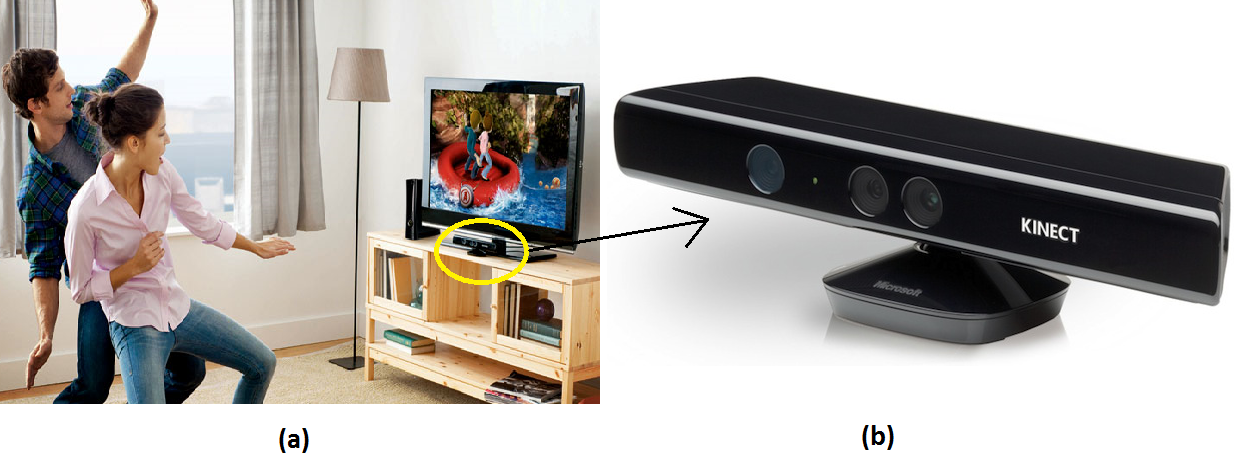
\includegraphics[scale=0.36]{sensorandtv}
\caption[The Kinect sensor]{The Kinect sensor (a) together with the rest of the needed equipments, and (b) alone}
\label{kinectsensor}
\end{figure} 
 
Kinect has not just experienced success as an entertainment device within the living room, researches have also started to see the possibility to use the Kinect for other non-gaming purposes, like within healthcare, education and industry. The key reasons for the broad use of Kinect are its accessibility and low price, in addition to the ground breaking technology it provides. The release of the Kinect for Windows \ac{sdk} is also a reason for the wealth of non-gaming applications, as it makes the the Kinect platform available for everyone to develop on \cite{microsoftnews}. 


\cleardoublepage
\chapter{Exergames for Seniors}
\label{chap:exforseniors}

\section{Related Work}
Exergames for elderly has become a popular topic in the past couple of years, and several research on how games can be developed for this particular user group have been conducted. It is quite common today to develop technology systems to a homogenous user group. This means that the characteristics of specific user groups, like the older user group, is being ignored. Elderly in particular, have some special characteristics that needs to be taken into account when developing technology systems for them. Most video games existing today have not taken these characteristics into account, and are therefore not suitable for this group. In this section, we will review some interesting literature on what to consider when developing technology systems, and in particular video games, for elderly.  

Billis et al. \cite{Billis} discuss some important issues that need to be taken into account when developing games for elderly. Elderly often suffer from decline in visual acuity, decreased audition, mobility changes and cognitive functions' decline. In addition, many elderly are not familiar with technology. The writers of the paper suggest that it should be possible to customize the game for every players' special needs. Font, size and color should be adjustable, and information should be provided in different multimedia alternatives, like text, voice and images. The objects should be of sufficient size and the elements should not move too fast. The overall interface should be as simple as possible, without the need to remember information given earlier in the gaming process, and it should be given sufficient information and guidance throughout the whole game. The game should also provide motivating messages to encourage the player. The writers also stress the importance of the social factors of the game, and suggest the ability to multiplay. At last, for the players to get interested and engaged in the game, the content of the game should match their cultural and lifestyle diversity \cite{Billis}.

de Bruin et al. \cite{bruin} write about the potential of virtual reality environment, with use of for example games, for exercise. Virtual reality platforms can provide naturalistic movements in a safe environment that can be customized after the patients' needs. It can offer a consistent program that enables for comparison over time. In addition, the use of games can distract the player from any pain they may have. For a game, stepping exercises can be suitable. They have found that stepping exercises can be a good predictor of falls, and it is proved that a repetitive training program with stepping exercises can improve balance in elderly. Also here, they express that the problem of already existing exergames is that they are too complex for the older user group. Therefore, there is a need to develop games specifically for this group where physical and cognitive limitations, as well as typical interests of elderly, are taken into consideration. The writers also present a study where it was shown that there was a significant decrease in relative \ac{dtc} of walking for elderly who was training physically combined with a VR dance game that required decision making, while training traditionally did not change this walking parameters. This comes from the fact that elderly often faces problems when they have to do more than one task at the same time \cite{bruin}.

Gregor et al. \cite{gregor} discuss the particular issues when designing for the older population, and propose a paradigm and methodology to support the process of designing software as close to the universal accessibility ideal as possible. These methods are called: \ac{d3} and a modified version of this: \ac{usid} \cite{gregor}.

The writers describe older people through three different groups:
\begin{itemize}
\item Fit older people: elderly who do not suffer from any diseases or dysfunctionalities, but who are different from when they were young.
\item Frail older people: elderly who in  general have a reduction in many of their functionalities and who often have one or more disabilities.
\item Disabled people who grow older: These are the people who have long-term disabilities which have affected their ageing process.
\end{itemize}

In addition, \cite{gregor} define some important characteristics of older people (directly drawn from \cite{gregor}):
\begin{itemize}
\item "The individual variability of physical, sensory, and cognitive functionality of people increases with increasing age".
\item "The rate of decline in that functionality (that begins to occur at a surprising early age) can increase significantly as people move into the "older" category".
\item "There are different, and more widely appearing problems with cognition, e.g. dementia, memory dysfunction, the ability to learn new techniques".
\item "Many older users of computer systems can be affected by multiple disabilities. Such multiple minor (and sometimes major) impairments can interact, at a human computer interface level to produce a handicap that is greater than the effects of the individual impairments. Thus research into accessibility focused on single impairments may not always appropriate solutions".
\item "Older people may have significantly different needs and wants due to the stage of their lives they have reached".
\item "The environment in which older people live and work can significantly change their usable functionality - e.g. the need to use a walking frame, to avoid long periods of standing, or the need to wear warm gloves".
\item "On a more positive note, older people can have access to a much wider experience and knowledge of the world than younger people, and a more mature approach to problem solving".
\end{itemize}

Most software design is static with no possibility to adapt to the different needs of the users. \ac{ucd} principles should be followed when designing technology systems. However, these principles have been developed for homogeneous user groups, and not for specific types of users. To make it easier to develop a technology system for the older user group with different characteristics, \cite{gregor} propose a modified version of the \ac{ucd} principles, which they call \ac{usid}. The issues this methodology address are \cite{gregor}: 
\begin{itemize}
\item "Much greater variety of user characteristics and functionality". 
\item "Finding and recruiting "representative users"". 
\item "Conflicts of interest between user groups (including "temporarily able-bodied")".
\item "The need to specify exactly the characteristics and functionality of the user group".
\item "Tailored, personalisable and adaptive interfaces".
\item "Provision for accessibility using additional components (hardware and software)".
\end{itemize}

As an example of the advantages of the proposed methodology, the writers present a case study that was developed at the Speech Project at Oxford Brookes University. In this case study they designed a web browser for people that were visually impaired. 200 visually impaired users evaluated the system.  The findings they did were: 
\begin{itemize}
\item Elderly seemed to lack confidence in handling IT systems. However, the confidence increased after they had experienced a successful interaction and decreased after experiencing an unsuccessful interaction.
\item Many elderly have difficulties remembering too much information. This indicates that there are important memory related factors that need to be taken into account when designing for elderly. 
\item Following a need for less information, will most likely also mean less functionality. From an other study they found that it was a need for the possibility that more functionality could be added after the user had mastered the initial, simple functionalities.
\item After some kind of assessment is passed, the user can be moved to a higher level. This can be done for example by self-assessment. To reinforce user-confidence the user should be able to reach goals \cite{gregor}. 
\end{itemize}

Gerling et al. \cite{gerling1} also discuss the chances and challenges when developing a game for the elderly users. They suggest four major guidelines that should be followed when designing games for elderly: \\
1. The player should have the possibility to interact with the game both when sitting and standing. \\
2. Avoid too extensive and sudden movements.\\
3. It should be possible to adjust the level when it comes to difficulty, game speed and device sensitivity. This changes should be possible to be adjusted by the player. \\
4. Interaction mechanisms should be simple, player frustration should be avoided, and the game should provide constructive feedback.

To verify these guidelines, the research group prototyped an exergame called SilverBalance. This game was made for the Wii Balance Board, consisted of two balance tasks and had the possibility to be played both sitting and standing. The game was tested on 9 seniors with an average age of 84. The following observations were made \cite{gerling1}
\begin{itemize}
\item All of the participants were able to play the game adequately. 
\item Participants expressed that the fact that the design was so minimalistic, made it possible for them to focus on the purpose of the game. 
\item The possibility to sit while playing the game was necessary because all participants were dependent on devices to assist them when standing and walking.
\item The players started to compare their results and comment on each others results, (suggesting that social factors are important.. slang på den selv jeg)
\item Impairments and diseases made it difficult for some participants after a longer period of playing, suggesting that alternative interactions should be included in such games.
\end{itemize}

The tesing of SilverBalance shows that the four criterions serve as good guidelines for developing games for elderly, (but that further research with the focus on the impact of age on different structural elements of games should be carried out. hva nå enn dette betyr?) \cite{gerling1}.

In another study Gerling et al. presents a case study where they introduce and evaluate a video game for elderly, called SilverPromenade \cite{gerling2}.  SilverPromenade is developed for the Nintendo Wii technology and utilizes the Wii Remote and Wii Balance Board. The game is stripped from complexity in functionality and design to be senior-friendly. The theme of the game is "a walk through the forest" and it can be played as a single-player game or a multiplayer game. In each mode of the game it is possible to engage three different roles.

The main concept of the game is the combination of the walk in the forest with optional mini games to engage the players. One player can be walking and solving the mini games, or the mini games can be used for multiplayer mode, engaging the maximum number of three players in SilverPromenade. The main task is to step on the Wii Balance Board to walk through the forest, \emph{the walker role}. The two mini games consist of catching a butterfly by pointing at it with the Wii Remote, \emph{the pointer role}, and counting rabbits by shaking the Wii Remote every time a rabbit appears on the screen, \emph{the shaker role}. The scenarios are simplistic, which is important when including elderly in digital game play. The concept of the game, "a virtual walk in the forest", appeals to elderly living in nursing-homes because it offers the possibility to "visit" the forest, which generally might be inaccessible for them.

Playing this game requires the older player to focus on cognitive, mental and physical abilities. They have to understand the basics of the game, they have to pay attention to elements appearing on the screen, and they have to be prepared for challenging situations. The person who has \emph{the walker role} has to continuously step on the Balance Board, which requires physical exercise.

SilverPromenade has an easy and understandable user interface that is intuitive also for people without any gaming experience. It consist of a menu structure which easily guides the user to the playing-mode. The input devices used for playing makes it possible for elderly to both sit and stand during game-play, which takes the different individuals abilities into consideration. Complex graphics and visual effects are avoided, while important elements are highlighted. If one of the three roles is not suitable, SilverPromenade offers the possibility of not including one or more roles.

A case study with SilverPromenade was executed on a group of frail elderly living in full-time nursing homes. The participants were asked to play the game and afterwards fill out a short questionnaire. During the case study they examined three research question related to interface design, game design, and player experience. Two groups of elderly participated in the case study, one group consisting of 9 seniors with prior experience with this type of technology, and one group with 9 seniors without any experience. The participants suffered from age-related changes, and most of them needed assistive devices to walk. During the game play they observed how the elderly used the controllers, how they understood the menu, and how easily they perceived the game behaviour. The gaming results were also observed.

Results from this case study show that there is a clear difference in performance between experienced players and inexperienced players, both in singleplayer mode and multiplayer mode. Experienced players clearly had an advantage. The one role that was handled equally well was the role of the shaker in singleplayer mode. Some observations done during game play was that some roles were difficult to execute. Players doing \emph{the walker roles} experienced difficulties with performing correct movements on the Balance Board, and players doing \emph{the pointer role} had difficulties using the Wii Remote because it requires that one point it directly towards the sensor. However, the results showed that the overall experience was positive. SilverPromenade gave an impression of being outside, and the use of a real-world scenario engaged elderly to play. The concept of the game lead to communication in terms of identifying objects, and helping and encouraging each other. One important observation was that the elderly where sharing and discussing their scores. The conclusion of the case study was that elderly enjoyed playing digital games, and that SilverPromenade could be an appropriate game to use in this age group \cite{gerling2}.

\section{Guidelines for Developing Games for Elderly}
\label{sec:summaryguidelines}
It is clear from the literature that elderly has some specific characteristics that need to be taken into account when developing technology systems aimed for them. Based on the reviewed research we will summarize important aspects when developing technology systems, and in particular video games, for elderly. In \cite{bruin} and \cite{gerling2} they discuss stepping as a relevant exercise for elderly. This is because this kind of exercise has proved to be a good predictor of fall and that repetitive stepping exercises can improve balance. In addition stepping, requires significant physical activity, which is important when improving physical health. We will not discuss this any further, as we are provided with relevant exercises from Cyberlab. Blabla. Kanskje det er tyoiske øvelser fra cyberlab, og da kan vi si noe positivt om det.

It is important to remember the limitations related to elderly users. We will now review and put together all of the different aspects discussed in the literature, that we found important. First we will list some of the typical characteristics of the older user. Then we will provide a list of relevant guidelines to be followed when developing user interfaces for elderly. 

\textbf{Characteristics of elderly people:}
\begin{itemize}
\renewcommand{\labelitemi}{$\bullet$}
\item Cognitive functions' decline, e.g. dementia, memory dysfunction, and the ability to learn new things \cite{Billis}, \cite{gregor}.
\item Decline in sensory functionality, like  visual acuity and audition \cite{Billis}, \cite{gregor}.
\item The problems elderly face, often increase significantly with increasing age \cite{gregor}.
\item Mobility change \cite{Billis}.
\item Needs and wants related to cultural and lifestyle diversity, as well as at what stage they are in life \cite{Billis}, \cite{gregor}.
\item Many are in need of assistive tools (for example when standing and walking) \cite{gregor}.
\item Inexperienced with technology. Many elderly seems to lack confidence when it comes to IT-systems. A better confidence can be achieved when experiencing a successful interaction with an IT-system \cite{Billis}, \cite{gregor}.
\item It is important to take into account memory related factors. Many elderly have difficulties remembering too much information \cite{Billis}, \cite{gregor}.
\item It can be hard to do two things at the same time \cite{bruin}.
\end{itemize}

\textbf{Guidelines:}

\begin{itemize}
\renewcommand{\labelitemi}{$\bullet$}
\item The game should have the possibility to be customized for every user's needs, condition, interests etc. This can be done by offering alternative interactions \cite{Billis}, \cite{gregor}, \cite{gerling1}.
\item Offer adjustable font, size and color \cite{Billis}.
\item The interface should have different alternatives for multimedia presentation (for example text, voice and images) \cite{Billis}.
\item The interface should be simple and not too extensive. The objects should be of sufficient size and there should be no sudden movements. Important elements should be highlighted \cite{Billis}, \cite{gerling1}, \cite{gerling2}.
\item Sufficient guidance and information should be given during the process, without the need to remembering earlier giver information \cite{Billis}, \cite{gregor}.
\item Constructive feedback should be given in a motivating form, to encourage play \cite{Billis}, \cite{gerling1}.
\item The story of the game should match cultural and lifestyle diversity. An example presented in \cite{gerling2} is a game with a real-world scenario, where the players have to walk through a forest. This seemed to appeal to elderly living in a nursing home, because they do not have the same possibilities to "just take a walk" in the forest \cite{Billis}, \cite{gregor}, \cite{gerling2}. 
\item Social factors should be included, by for example offering the possibility to multiplay \cite{Billis}, \cite{gerling2}, \cite{gerling1}.
\item It should be offered variety in user characteristics and functionality \cite{gregor}, \cite{gerling1}.
\item The game should not have too much functionality, but instead offer the possibility to add more functionality after the existing functionalities are managed \cite{gregor}, \cite{gerling2}.
\item Offer different levels with different difficulties. With this comes the possibility to reach goals. The device sensitivity and the game speed should also be adjustable \cite{gregor}, \cite{gerling1}.
\item It should be possible for the player to adjust levels themselves \cite{gregor}, \cite{gerling1}. 
\item It is important during the development to test on representative users \cite{gregor}.
\item The possibility to interact with the game both when sitting and standing is important \cite{gerling1}, \cite{gerling2}.
\end{itemize}







\cleardoublepage
\chapter{Characteristics of Video Games}
Game designer Sid Meier came up with one of the most famous definitions of game: “A game is a series of interesting choices” \cite{understandingvg}. This of course, does not apply for every video game. In \cite{understandingvg} the authors present the MDA-model, which was developed by Robin Hunicke, Marc LeBlanc and Robert Zubeck, after several workshops conducted at the “Game Developers Conference” in California between 2001 and 2004. This model divides games into three elements: mechanics, dynamics, and aesthetics, and is a very useful tool for designers to understanding games. Mechanics are not something we can see or hear, but rather the rules and basic code of the game. It is for example the algorithms that lies in the ground for creating the reaction pattern of a computer-controlled character. Dynamics is based on the mechanics and describes what events do and can occur during the gameplay, seen from the players point of view. Aesthetics say something about the emotions triggered when interacting with the game. A list of elements  that attract us to games is provided in the book (directly drawn from the book): \\
- Sensation (game as sense-pleasure)\\
- Fantasy (game as make-believe)\\
- Narrative (game as drama)\\
- Challenge (game as obstacle course)\\
- Fellowship (game as social framework)\\
- Discovery (game as uncharted territory)\\
- Expression (game as self-discovery)\\
- Submission (game as pastime).\\
One or more of these can be included in a game, but not all of them \cite{understandingvg}.

(I denne boken presenterer de fire sjangere av spill: action games, adventure games, strategy games and process-oriented games. Jeg klarer ikke helt se hvor exergames faller under, men om det måtte være noen blir det den siste. skriver ikke noe om det ennå, ettersom det ikke virket veldig relevant. )

\section{Aesthetics}
The aesthetics describes everything that can be experienced by the player. These are the elements that actually makes the game. The aesthetics can be divided in three, namely rules, geography and representation, and number of players. The rules say something about what the players can and cannot do, as well as what actions will make the score increase or decrease. The geography and representation element says something about how the video game is represented through graphics and sound. Here there are a lot of different design possibilities. The number of players is important, because there are huge differences between a single-player game and a multi-player game. This is an important choice because it affects a number of game elements. In a single-player game artificial intelligence (AI) is important, because the player has to play against the computer and not real humans. The computer can never be as intelligent as the human brain, and generally employ a very limited set of strategies. Therefore, it can be easy for an experienced player to win over the opponent. When designing multi-player games, artificial intelligence is not needed, as the player will play against other human players. These games faces other issues instead. For example it has be possible to distinguish between characters. This can be done by giving them different unique features, but at the same time not make any character superior. It is also important to facilitate social interaction between the players, like for example cooperation or competition \cite{understandingvg}. Often in multi-player games, it is possible to chat with the opponents or team members.

We will now look a little closer into the three categories rules, geography and representation, and number of players.

\subsection{Rules}
In \cite{understandingvg}, they distinguish between two types of rules; interplay rules and evaluation rules.The former are the physical laws. It determines what properties the different elements in the game should have, as well as the actions that can be done, as well as what will happen corresponding to the action action. An example of this is “What will happen when the player presses button A? Jump”. The latter defines what will happen when an action is made. For example if an action will be rewarded or punished \cite{understandingvg}. In \cite{understandingvg} gameplay is defined as “the game dynamics emerging from the interplay between rules and game geography”. The dynamics can be of different types. They can be entertaining or they can be predictable, or they can not be any of those. 

\subsection{Geography and representation}
Geography and representation is about how the game is represented through graphics and sound \cite{understandingvg}. Graphics and sounds are used to set the games environment and enhance the players enjoyment of the game, but has no effect on how the game is played.Graphics is needed in a videogame to in a best possible way imitate reality and enhance the player experience. This means that instead of telling out what is happening, it will be shown visually. Sound is important in video games for the same reasons as why graphics is important. Background music can set the atmosphere of the game, as well as give an indication on when actions will change and if the atmosphere is changing (for example from happy to sad). Sound can also be used as feedback to the player \cite{umlapproach}. There are different types of sound included in a  video game. \cite{understandingvg} distinguish between four categories:
vocalization, which is the game’s characters’ voices,
sound effects, which are sounds made by the different objects in the game, ambient effects, which is non-specific sounds that makes the atmosphere in the game, and music, which is the game’s soundtrack, but also a part of setting the atmosphere. The latter is a very important part of the game. Other elements that can affect sound effects are the environment, spatiality and physics. What kind of environment the player is in can affect the  sounds. An example of this, is what kind of floor the characters are walking on or weather conditions. The sound will also be affected by where in space it will come from. For example, a sound from far away sounds different from a sound close up. In addition, sound will be affected by movements. Imagine the sound of the sirens on an fast passing ambulance.

There are many things to consider when it comes to how the game should be represented. Ta med tabell side 107.  It has to be decided if the game will be in 2D or 3D and in first-person or third-person. Two-dimensional graphics are represented by only two coordinates and does not have any depth. This makes a very unrealistic scene. Three-dimensional graphics, on the other hand, has depth, and is therefore much more realistic. Every game will either have a first-person perspective, a third-person perspective, or a mix of both. In a first-person perspective, the game is played through the characters eyes, while in a third-person perspective the player can see the character he controls through the game. Games will also either have an isometric perspective or a top-down perspective. Isometric perspective is when three-dimensional objects are presented in a two-dimensional form, like in a architectural drawing, while a top-down perspective is, as the name suggest, when the scene is shown from above. The choice of perspective is important because it decides how the player will perceive the game world. It is also important to choose the right perspective with the right dimension. A third-person game can be played in a two-dimensional and a three-dimensional space, while a first-person game should only be played in a three-dimensional space \cite{understandingvg}. Another aspect experiences by the player is time. It is proposed to distinguish between play time and event time, where the former is the time a player uses playing the game, and the latter is the time in the game world. If play time and event time are the same, we can say that the game is played in real time. In many games it is possible to save the game, and return to the same state at a later time \cite{understandingvg}.

There are many different ways to present a game graphically, and Aki Järvinen defined three different styles common for video games. \\ 
Photorealism: “a style of painting that tried to completely mimic photographs”. There are two subcategories of photorealism: \\
Televisualism tries to give the same visually look as shown on the television. Typical for this, can be for example football games. Illusionism is the other category. Here it is used photorealistic graphics in the service of non-realistic content (siste setning skrevet av. skjønte ikke helt). \\
Caricaturism: Here the use of so called caricatures are used. Caricatures are drawings that presents an object by exaggerating the prominent features of the object, and often gives the feeling of a cartoon. \\
Abstractionism: In this category there are no real people of real-life objects involved. Instead  the game has a rather abstract form. An example of this is the well known game Tetris. A problem with these kind of games is that they often face a hard time on the market. This is because humans mostly get attracted by the story, and it can therefore be hard to create attention just around the mechanics of the game. Therefore, it is within this category very important with the story \cite{understandingvg}. 

\section{Story}
One important element of a videogame is the story, or the narrative. The story is included in the game to make the involvement and enjoyment better for the player. The story is just a part of the game, and is not the game \cite{umlapproach}.  Different events make up the narrative and will usually contain settings and characters \cite{understandingvg}. Unlike literature and film, which centers on the story, the game centers on play. Therefore, the narrative should be looked at in a player-centric context (Towards a Game Theory of Game, Pearce). The game designer is kind of creating the story together with the audience. This is because the player often make their own story throughout the game \cite{umlapproach}. This means that the game designer creates the background storyline, while the player creates the experimental story while interacting with the game or others. 

In \cite{understandingvg} they introduce interesting elements of narrative in video game, and discuss three different categories: “The fictional world: settings and actors”, “Mechanics: organizing narrative action”, and “Reception: the player’s experience of story”.

The fictional world: settings and actors can also be thought of as who and what. The game space, which is the game settings, is on of the most important parts of a game. The game space is a reproduction of some of the features of the real world and contains specific rules to make it possible to play the game. There are different characters in a game, and they are very important for the story. This includes not only the characters that the game is about, but also characters that make things happen and that interacts with the main characters. Therefore, all the different characters need to be considered. \cite{understandingvg} propose four different categories of characters: \\
-Stage Characters: These characters can not be interacted with, and serve more as just a part of a scenario. \\
-Functional Characters: These are also just a part of a scenario, but in addition, they have a general function, which makes it possible for the player to interact with them in some way. \\
-Cast Characters: These have specific functions in the game that has something to do with the story. \\
-Player Characters: These are the characters that the player is in control of. 

The different characters can be constructed in different ways. They can be constructed through description, which means through the way we can see them on the screen. This can be done in a symbolic, naturalistic or a “real-life” way. See table blabla for examples.

her skal det være en tabell

The characters can also be described through their actions, through their relationship to space, through other character’s views, or just through a meaningful name. The player character is the most important type, and was by Toby Gard divided in three different categories, in accordance to how easy the player will identify with them, avatars, actors and roleplaying: 

“Avatars are a non-intrusive representation of ourselves, actors are always part of a story (or have a story, albeit minimal sometimes), and roleplaying characters have very different abilities that we can raise according to our performance”. \cite{understandingvg} 

With the use of avatars the game is in first-person and can therefore not be seen, while actors usually will be seen in third-person. In addition, actors will usually have a personality and they are well integrated in the story, while an avatar usually do not have a personality at all. Roleplayers are quite different. Here the player create their own characters. The player can choose their name, and their abilities, as well as if they want to play in first-person or third-person.  

Mechanics: organizing narrative action can also be thought of as how the action of the story is organized. There is a basic concept for how to organize the story in a game, which is called “branching”. This means to have multiple paths in the story. 
Ha med figur 8.5 på side 181 i boka: a model of classical linear fiction. 
The figure shows the standard progression of a story of linear fiction. In traditional stories, it goes through a resolution. This can not be applied in a game, because it would not let the player do anything. Therefore, another model is applied for a game:
Ha med figur 8.6 på side 182: a model of interactive fiction
This model has no continuous curve. In this model it is more about finishing each chapter by solving puzzles, and relies on the emotional satisfaction the players get from the victory of solving a puzzle. Even though an action in a game can lead to different endings, the player is actually solving a story. These games are called progression games because the player has to finish different actions, before proceeding. The different chapters are cummulative, meaning that each chapter are building on each other. Very common in these kind of games it is a climax or a resolution at the end of each chapter (in many games you have to fight “the boss”). 

The other structure of narratives, is emergence games. This structure depends on a more active artificial intelligence where all the objects in the game has behaviours (Example directly drawn from the book: In a progression game, the dragon will always attack the player when she steps into the cave, but in an emergence game, this might depend on how the player behaves towards the dragon, which is a more “active” object with a few possible different responses. Some game designers (Smith and Juul) means that an emergent structure is preferable in games. This is because this structure gives the player more freedom. To be able to easily explore the smaller events in a game, game designers are making so called “quests”, which is the submission the players have to perform in the game. When the different quests are defined, it can be put together and be told as a story. In \cite{understandingvg} that say that “ideally, quests are the glue where world, rules and themes come together in a meaningful way”. Quests can be seen differently from the designer perspective and the player perspective: The designers look at quests as “a set of parameters in the game world (making use of the game’s rules and gameplay) that creates a challenge for the player.”, while the players look at the quests as “a set of specific instructions for action”. 

Reception is how the players experience a story. In \cite{understandingvg} they argue that: ”a reception-theory based analysis can explain the way that narrative and gameplay together determine the player experience in games that make use of stories”. We will not describe this theory any further here.. blabla.. 

\section{Gameplay}
NB: dette delkapittelet skal merges litt med tidligere delkapitteler. Er fra en annen kilde, så bruker en del andre begreper.

In a video game, everything really depends on the gameplay. Gameplay defines how the game is played and is the most important element of a game. In short, gameplay can be describes as the interaction between the player and the game. Siang. et al. describes two different kinds of interactions: player-object and object-object. When creating a game, a set of rules about what kind of interactions can be made have to be set. These rules are set by determining what kind of interactions are allowed between the two components: players and game objects. The paper describes the player-token interactions with this model:
figure “the player-token interaction”
which is a description of gameplay, set aside the players experience. 
Different from objects is that tokens are conceptual (hva betyr det?), and may not have a one-to-one mapping with the programming language (skrevet rett av, vet ikke hvor viktig det er).
In a video game tokens is a thing that can react with something in a game. It can be defined three categories of different tokens: static, dynamic and behavioural. Static tokens has the same visual look throughout the whole game. Dynamic tokens, also called entities, can react to certain events in a game. Behavioural tokens are the parameters how they will react to the player and other tokens and are not physically represented in the game. Example is a game level manager which tells the player about high scores etc. The tokens can have attributes, which is representing the tokens state. Example of an attribute is the number of life. The tokens can also have behaviour, which say something about how the token can react in certain events \cite{umlapproach}.

\section{User Interface}
The interface is there to enable interaction between the player and the token. In their paper Siang et al. present a figure describing the gameplay:

figure

The interface is where and with what the player interacts with the game and includes the input that is sent through the input devices, like a game console, and the output the user receives on the screen and the speaker \cite{umlapproach}.

\cleardoublepage
\chapter{Usability}
\section{Usability}
Usability says something about how easy it is to use, learn and understand a human-made system. Examples of systems can be a machines, software applications, websites, tools, or anything else that involves human interaction with an object. Usability is a often used in association with technology development, in terms of making digital systems understandable and intuitive for the users through user-friendly interfaces. Usability has played a huge part in the evolvement of bringing digital systems into people’s homes and everyday life. The first computers and digital systems that were developed consisted of complex and not understandable applications that only professionals with special knowledge could use. There was little focus on simple and accessible systems, and complex interfaces were actually appreciated and gave the system credibility. First, when computers and digital systems were developed with the intention of being used by the normal user, developers had to think about usability. The developers had to put the user in the center of the computer system, and not only focus on functionality and system features \cite{mmi}.

Usability is a wide and quite abstract term, and it is not easy to understand, to measure, or to practise right. There is no definitive solution on how to make a good and user friendly system, and it is challenging and time consuming to find the users needs. For a system design to experience success interaction designers has to pay attention to various aspects of the user. The best way to do this is to involve users in the process of developing the system, from requirement definition and the design phase, to prototype and system test, all to the end of the system's lifecycle \cite{mmi}. When creating something completely new, it is all about understanding what the users want and need, but often the users themselves do not know what they want. It will not be possible to walk up to a potential customer and ask what he or she wants and needs. This does not mean that a developer should be creative, come up with a great idea and bring it into life without ever talking to the user group. The development of a new system should be done as a cyclic process, where development and user involvement goes hand in hand \cite{mmi}.  
\begin{figure} [ht!]
\centering
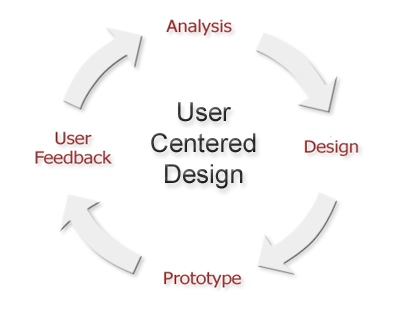
\includegraphics[scale=0.8]{userdesign.jpg}
\caption{User Centered Design \cite{userdesign}}
\label{userdesign}
\end{figure}

Making good, intuitive, easy to understand systems is essential for a system to be successful, accepted and used. "Make it or break it" is a slogan that connects well with success and acceptance. A system can possess the best functionality there is, but if the users do not understand how to use it, the system will fail. An example of this is Apple's huge breakthrough when they launched their iPhone in 2007 \cite{iphone2007}. One might associate the invention of the touch phone with Apple's iPhone, but the truth is that touch phones was invented long before the iPhone. The first touch screen was published as early as in 1968, where it was used for air traffic control. In the early 1990s IBM released their Simon, which was the first smart phone with touch screen technology \cite{touchphone}. Apple was also eager participants in the development of touch screen devices. Already in 1983 Apple had a prototype of a touch screen phone \cite{applefirst1983}, and in 1993 they released the world's first Personal Digital Assistant (PDA), called Newton \cite{touchphone}. Apple’s success with their iPhone is based on focus on user’s needs throughout the development process, which has resulted in good, intuitive and user-friendly design and interfaces. "KISS" and "Less is more" is other terms related to usability. "KISS" is an acronym that stands for "Keep it simple, stupid". This term was used in the US navy in the 1960's, and it was a principle stating that simple systems work best than complex ones. The KISS principle has been adopted into the subject of design and usability. Simplicity should be the main focus in design, and every element that leads to unnecessary complexity should be avoided [KILDE - wiki foreløpig]. Ludwig Mies van der Rohe was a German architect that used the term "Less is more" to describe his extreme simplistic and minimalistic design style, and his use of that term became a guiding principle in modern design. "Less is more" has also been widely used as a slogan in association with usability. \cite{rohe}. Minimalistic design can be described as "design at its most basic, stripped of superfluous elements, colors, shapes and textures." With minimalistic design, the most important elements are brought into focus. In this way the user will not be distracted from, or miss out on, the content that is important \cite{lessismore}. Also big companies, like Microsoft, focus on simplicity in their design. Microsoft has launched an article called "The Importance of Simplicity" in their developer network, about how to design user-friendly systems while still keeping good functionality. Microsoft present a topic called "Simple Can Be Powerful". This means that simplistic design not necessarily implies lack of functionality. Simplistic design will provide ease of use for first timers. The idea is to present a design that is intuitive, understandable and easy to learn, but that has the opportunity to build up knowledge about the functionality needed. A possible solution could be to include customisation so the users can set up their own workspace \cite{msdnsimple}.             

We have experienced a great shift in technology from the first computer was invented and until today. Technology has been more mobile due to laptops, smart phones and other portable devices, and it is also used more often because of instant messaging, e-business and social networks \cite{mmi}. Users are no longer just "computer professionals", but normal people in all age groups, with different skills and interests, that are both experienced and inexperienced with technology. This has been possible because of designers and researchers with focus on human needs. The term human-computer interaction was created, which is about including psychology in developing human-centric design. This is not an easy task, and it includes people from a many different sciences. Ben Shneiderman list “psychologist, instructional and graphic designers, technical writers, experts in human factors or ergonomics, information architects, and adventuresome anthropoplogists and sociologist” as some of the people to be included in the process of saying something about usability and human-computer interaction \cite{mmi}.    

The work for an interactive system designer is as mentioned to combine the sense of what attracts users with system functionality. To help interface designers make successful systems, a theory called the four pillars of design has been developed. This theory does not guaranteed brilliant systems, but it could be helpful along the way in making good, successful systems. The four pillars of design consist of “user-interface requirements”, “guidelines, documents and processes”, “user-interface software tools” and “expert reviews and usability testing” \cite{mmi}.    

\emph{User-interface requirements (Ethnographic observations)}\\
A major key to success when developing a system is connected to specifying the user requirements, and how well these requirements are defined and understood.  The way to specify requirements differs from organisation to organisation, but what the final results should always include the same; Who should use the system, where should it be used and what should it be used for. In addition to this, functional requirements (system requirements like hardware,  software etc.) and non-functional requirements (requirements saying something about the user interface, like functionality, input devices, etc.) should be specified and decided \cite{mmi}.

\emph{Guidelines documents and process (Theories and models)}\\
It is important for the interactive system designer to generate a document that obtains a set of guidelines which specifies how the design should be. Companies like e.g. Apple uses guidelines documents to specify design principles developers should follow. This is to create consistency in design across systems and products. Design may differ as different systems has different needs, but there are still some elements that should be considered in the guidelines document. The documents should contain guidelines for:

\begin{itemize}
\renewcommand{\labelitemi}{$\bullet$}
\item Words, icons, and graphics.
\item Screen-layout issues.
\item Input and output devices.
\item Action sequences.
\item Training.
\end{itemize}

The procedure of creating these guidelines should be done by including different parts of an organisation. It should be a social process, this to gain visibility. It is important that the guidelines are flexible, so that they can adapt to changes in needs and experiences \cite{mmi}. 

\emph{User-interface software tools (Algorithms and prototypes)}\\
In the early stages of development, it is difficult for users to picture what the final result will look like. This may lead to situations where the system design is finished and the users are left with the feeling of not being satisfied. This would be a problem, because of the high cost associated to make changes in implemented systems. One way to address this problem is to let the users get a realistic impression of the final result early in the development process. This could be done by presenting different types of prototypes. These prototypes could be simple sketches on paper, a display proposal or a presentation with use of PowerPoint. 
When deciding on which development environment to use, there is a number of good products to choose from. Most of them are easy to use, and offers good features. The important part is for the developers to choose the development environment that is most suitable for the product they are going to make, due to performance, cost, and how easy it is to use and learn \cite{mmi}.
	
\emph{Expert reviews and usability testing (Controlled experiments)}\\
To be able to launch a successful system, it is important with testing along the way in the development process. System testing could involve both experts and the intended users \cite{mmi}. 

With the importance of user friendly technology systems, as well as user involvement, in mind, we will move on to the next chapter, where we will describe the methodology used in this thesis. 
\cleardoublepage
\chapter{Methodology}
When developing technology systems it is important to involve the user in the process to make something that fits the users needs and wants. Data collection is a key role to gather information about the users needs and to establish requirements to the systems. The primary methods used in this thesis are experimental simulation, and qualitative research methods like participatory observation and focus group interviews. In addition, support methods like video and audio recording, and a survey are used. The latter was used to in an efficient way gather information about  who the informants were, and their attitudes towards exercising and technology in general. We arranged two sessions, which we have called workshops.  The definition of a workshop is "A meeting at which a group of people engage in intensive discussion and activity on a particular subject or project" \cite{dictionary}. This definition fits well with both our sessions. Workshop 1 was organized as an experimental simulation, as defined by McGrath \cite{McGrath}. We invited a group of relevant users to participate in a setting that we tried to make as natural as possible. Experimental simulation will be described in more detail in Section \ref{sec:experimental} The execution of workshop 1 will be described closer in Section \ref{sec:ws1}. Based on the findings from workshop 1, in addition to findings done in the literature, we developed requirements for a video game concept, and made low-cost/low-fi prototypes. This concept was presented by the use of prototypes, story telling and acting, for a potential user group. The users were engaged to discuss the concept in a focus group. This session is called workshop 2.

In the first part of this chapter we will give an overview of the importance of user involvement, and the relevant research strategies and methodologies used in this thesis to meet the requirements of user involvement. We will also discuss ethical challenges and the different criteria for the quality of the research. At the end of this chapter we will give a thorough presentation of the execution of the two workshops conducted in this thesis. 

\section{User Involvement}
There is no definitive solution on how to make a good and user friendly system, and it is challenging and time consuming to find the users needs. For a system design to experience success interaction designers have to pay attention to various aspects of the user. The best way to do this is to involve users in the process of developing the system, from requirement definition and the design phase, to prototype and system test, all to the end of the system's life cycle \cite{mmi}. ISO 9241-210 describes why it is important to include users in system development \cite{dis20109241}:

\emph{"Involving users in design and development provides a valuable source of knowledge about the context of use, the tasks, and how users are likely to work with the future product, system or service. User involvement should be active, whether by participating in design, acting as source of relevant data or evaluation situations [...]"}

User involvement focus on finding future users of the system to be made, and let them take part in decision making during the development process \cite{bjerknes1995user}. User involvement provides the opportunity for developers and future users to meet and discuss topics and issues related to the system. This gives the users knowledge about system features and functionality, and it makes it possible for developers to get to know and understand their potential users. Participation in the development process will give users the possibility to influence how the final system will be. This could lead to a feeling of ownership, which again will increase the probability for users to accept and employ the final system. User involvement will also increase the probability for developers to make good and user-friendly interfaces \cite{infodesign} \cite{mmi}. 

When creating something completely new, it is all about understanding what the users want and need, but often the users themselves do not know what they want. It will not be possible to walk up to a potential customer and ask what he or she wants and needs. This does not mean that a developer should be creative, come up with a great idea and bring it into life without ever talking to the user group. The development of a new system should be done as a cyclic process, where development and user involvement goes hand in hand \cite{mmi}.  

\begin{figure} [ht!]
\centering
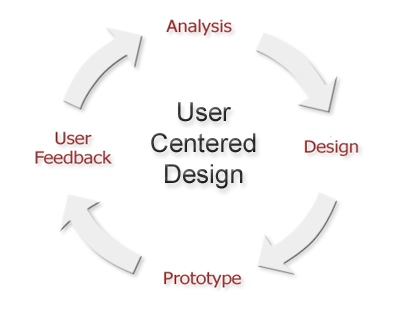
\includegraphics[scale=0.8]{userdesign.jpg}
\caption[User centered design]{User centered design \cite{userdesign}}
\label{userdesign}
\end{figure}

The importance of user feedback throughout the development process is stated in ISO 9241-210 \cite{dis20109241}:

\emph{"Feedback from the users is a critical source of information in human-centered design. Evaluation designs with users and improving them based on their feedback provides an effective means of minimizing the risk of a system not meeting user or organizational needs (including those requirements that are difficult to specify explicitly).  [...] User-centered evaluation should also take place as part of the final acceptance of the product to confirm the requirements have been met. Feedback from users during operational use of identifies long-term issues and provides input to future design."}

\subsection{Use of Prototypes}
\label{sec:prototypes}

This may lead to situations where the system design is finished and the users are left with the feeling of not being satisfied. This would be a problem, because of the high costs associated to making changes in implemented systems.

These mock-ups or prototypes could be simple sketches on paper, a display proposal or a presentation with use of PowerPoint.

\section{Choosing the Setting for Our Study}
\label{sec:experimental}
When doing research there are three criteria you would like to maximize \cite{McGrath}, \cite{alsos}: 
 
A: Generalizability of the evidence, \\
B: Precision of measurements, and \\
C: Realism of the study context.  

However, it is not possible  to maximize all three criteria because if you do something to increase one criteria, you are likely to decrease an other criteria. In our study realism is the most important criteria and is the one we want to maximize as much as possible.

There are different research strategies that can be used. Sometimes it is hard to find one that fits exactly to what you as a researcher want to do.
\begin{figure}
\begin{center}
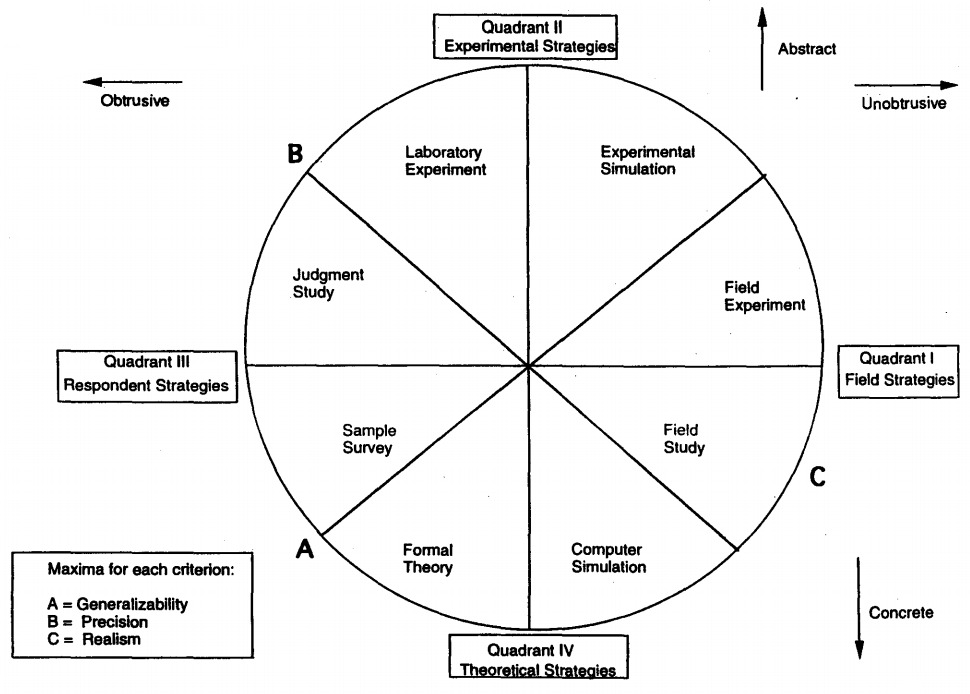
\includegraphics[scale=0.5]{circumplex}
\caption[The strategy circumplex]{The strategy circumplex \cite{McGrath}}
\label{fig:circumplex}
\end{center}
\end{figure} 
The strategy circumplex by McGrath is shown in Figure \ref{fig:circumplex}. This figure presents eight different strategies \cite{McGrath}. As can be seen from the figure the different strategies are arranged in a way on whether they are abstract versus concrete, and obtrusive versus unobtrusive. The figure also shows at what strategy the three different criteria, A, B and C, are at their maximum. We studied this circumplex to find where our study fits in. We found one of the strategies from quadrant 2 appropriate. Within this quadrant there are two different strategies, laboratory experiment and experimental simulation. In the former strategy the researcher put together a setting and invite some individuals to enter the setting and act by the defined rules. Here the researchers typically know what behaviour they are looking for and can within this setting study this with precision. The second strategy is experimental simulation. At the same time as trying to get the precision, as in a laboratory experiment, the researcher also try to get some more realism than the strategies in quadrant 1 do. This means that the researchers are setting up a situation like in the laboratory experiment, but at the same time are trying to get some realistic behaviours from the participants. This means that the researchers try to get sufficient realism, and at the same time keeping precision and control. The field experiment strategy within quadrant 1 was also considered because we found it in some ways to fit for our study. This strategy, compared to field study which has maximum degree of realism, opens up for being a little more obtrusive, and in that way give up some of the realism. We wanted to create an as natural setting as possible, and to implement the study in a place familiar to the informants. However, as defined in \cite{McGrath}:  \emph{"The essence of both of the strategies in quadrant 1, the field study and the field experiment, is that the behaviour system under study is "natural", in the sense that it would occur whether or not the researcher were there and whether or not it were being observed as part of a study"}. In contrast, the behaviour gotten from the two strategies within quadrant 2, would not have been apparent if it was not for the researchers doing the study, which is the case in our study. Therefore, we conclude that we in our study uses some variant of experimental simulation, even though no study is fully under only one strategy. It is important to understand that even though experimental simulation is less realistic, the study is still real and the behaviours gotten from the participants are real, however influenced by the setting \cite{McGrath}. Because the experimental simulation never can be as realistic as the field study, there will be an error in the information gathering, which can pose validity issues \cite{alsos}. The validity of our research will be discussed in more detail in Chapter \ref{chap:discussion}. We will now discuss research methods used to gather data from the experimental simulation. 


\section{Qualitative Research}
Qualitative research is a method used to get an in-depth understanding of a phenomenon. This research method is well suited when studying sensitive and personal topics, as well as when studying topics that there have not been done much research on. Interpretation is very important in qualitative methods, as well as flexibility and openness. With flexibility it means that the scheme should have the possibility to be changed during the research, if needed. The focus in this research method lies on how and why things are done, and not how many who does it, like in quantitative methods. Quantitative methods include huge samples, while qualitative research can give more information about a small sample \cite{qualitative}. This often result in a close and personal relationship with the people being studied \cite{tjora}.  \\ \\
The qualitative research process can be divided into phases, that partially overlap. The first phase consists of defining what the research will find out. We have done this be defining some research questions which can be found in Chapter 2. The next phase is the data gathering phase. This phase can be performed with several methods. The following phase includes interpreting and analysing of the data, as well as formulating theories. In the last phase, the results will be presented. Data gathering and analysis should be done in parallel. In that way, further data gathering can be adjusted from what have found in earlier analysis. There are four different data gathering methods described by Thagaard in \cite{qualitative}:

- Observation \\
- Interview \\ 
- Document analysis, and \\
- Analysing of video and audio recordings

The most common methods are interviews and participatory observation. These are primarily the two methods we have used in our thesis. It is common in qualitative research to have a close connection between the researcher and the people who is being studied. This especially apply in interviews and observation. This contact is important for the data the researcher will gain from the study \cite{qualitative}. The interview method and the observation method will be described in more detail later in this section.

In most qualitative methods it is common to textually document the data which is being analysed. The documentation can include what people do, their statements, their intentions or their perspectives. The text can be notes from the field or printouts of  recorded interviews \cite{qualitative}. In this thesis we have textually transcribed video and audio recording, and used  \ac{sdi} to analyse this data. This will be discussed later in this section.

\subsection{Ethical Challenges}
The close contact established between the researcher and the informants introduces some ethical challenges. All results conducted from the research needs to be precisely and correct when presented. This also includes other researcher's work. Plagiarizing means to copy other people’s work and take credit for it. This is illegal, and it is therefore important to properly state the resource of the information that is being presented.  When working in close contact with informants, the researcher often gets personal information about the informants. Personal information means information that can be linked to individuals. In projects with this kind of information, the project needs to be reported. In the case of research projects performed at universities, the project needs to be reported to \ac{nsd}, which is an entity in care of data protection for these institutions. \ac{nsd} will evaluate each project in accordance to research ethical rules \cite{qualitative}. In this thesis we will do observation of a fixed workshop, as well as focus group interviews with the participants of the workshop. This will require having a close connection with the participants, as well as gather personal information about them. In addition, we will video record the workshop and audio record the interviews. Therefore, this thesis has been reported to \ac{nsd}, see Appendix X. 

\subsubsection{Ethical Guidelines:}
Tjora \cite{tjora} suggests that common politeness should be a basis for ethical research. However, some additional rules needs to be followed. These are described in the following guidelines:

\emph{Informed Consent:} \\
In a research project with people involved, there is a requirement that the researcher has the participant's informed consent. This means that the informants have gotten all the information they need to know about the participation, have self chosen to participate, and that they can withdraw at any time without any consequences. One challenge about this, is that in some projects too much information can affect the participants behaviour (for example if the participants know too much about what the researchers are looking for, they can act differently) \cite{qualitative}. Because of the setting of our workshop we did not see this as a problem for our research, so the participants were well informed on what we were researching. To get participants to our study we held a presentation for a group of relevant people, where we described the project and the workshop. In addition, all participants, got an invitation letter, with a short description of the project and information about what they were going to participate in, and their rights. Every participant gave us their written consent to participate. The presentation, invitation and written consent can be found in Appendix Y.   \\ \\
\emph{Confidentiality:}\\
Researchers are required to keep all the information they collect about a participant confident. This means that the information have to be anonymized. This also involves strict requirements to how personal data, that makes it possible to identify individuals, should be stored and annulled. There are rules about how long data can be stored. General principles are that data should be stored for only the amount of time there is use for the data, and that data which can be directly linked to an individual should be stored separately and not electronically.  Reuse of data is not allowed without consent from the participants \cite{qualitative}. In this thesis we have signed a non-disclosure agreement to assure the participant that we will not reveal any confident information about them. This is found in appendix Z. In addition, we have assured the participant that all data we collect will be deleted within 3 years after the project's end. See Appendix Y. \\ \\
\emph{Consequences of participating in research projects:}\\
The researcher has responsibility over the participants safety and should respect their wishes. It is important to have thought through what consequences the execution of the research may have for the participants. The researcher is required to protect the participant's integrity during the process \cite{qualitative}. In our workshop, all participants were allowed to choose what they were comfortable with doing and not doing. They were allowed to withdraw at any time without any consequences.  \\ \\

\subsection{Observation}
Observation, often called ethnography \cite{tjora}, is used when the researcher wants to see how a group of people behave in a specific setting \cite{qualitative}. With observations the social world will be studied in its natural setting, to get a real and natural view of the world. The researcher can understand what people actually do, instead of just getting what the people say they do (like in an interview) \cite{tjora}. When doing observation, one important decision is how the observer will perform in the field. This varies from project to project. The observer can be a participant or just an observer, and the observation can be open or undisclosed. Participatory observation is something in between being a complete observer, where the researcher keeps himself in the background, and s complete participator, where the researcher participates in the same way as the informants. This involves the researcher being present in the setting of the participants while observing how they act. The researcher participate in the session, in the sense of interacting with the participants while they are performing the tasks. This means that the researcher does not do the same as the participants. Participation observation is well suited in research of a new and immature topic \cite{qualitative}, which is what we have done.

It is very common to combine observation with interviews. This is for the researcher to verify or discard the understanding he or she has acquired during the observation. In most research it is important to study the behaviour in the informants own environment. This will give a more natural behaviour. However, it is important to acknowledge that the informants may not find the environment "natural" when the researcher is observing them. How the researcher presents the project to the informants is important to gain interest among the people they want to observe. The researcher should in a trusting way, present him or herself and the project \cite{qualitative}.

In this thesis we have used observation as a method for understanding how seniors interact with commercial Xbox Kinect games. This does not fall under the immediate understanding of the definition of observation, as this is to gain understanding of "a natural world" \cite{tjora}. This is rather a future scenario of a possible "natural world". The planned exercise game was in our previous study \cite{project} evaluated to suit well into a clinical setting at the physiotherapists' office, or/and in a group training session. Therefore, we tried to create an as realistic small group training session where 4 people played alone and together in the same room.  We wanted to see how the seniors were interacting with the game, as well as their reactions to different events. The workshop was held in the premises where the organization "Seniornett", which they all were members of, have their meetings. We did this, to make the setting as natural as possible.  However, in this case, it was not a natural environment where they "normally play a game", as none of the participants had played these kind of games before. This is why we have defined this session as an experimental simulation. However, we evaluate the setting, to be as natural as possible at this time.  During the observation we looked for things that support what we have read in the literature, as well as for new aspects that we were not aware of (see our research questions presented in Chapter 2). This was for us to get an understanding of what works, and what does not work with existing commercial Kinect games. This was used as a foundation for the development of a new game concept. 

\subsubsection{Video Recording}
Workshop 1 and 2 were video recorded. An advantage about using video as a tool for observing a situation is that you get a detailed representation of what happened in the situation. Together with the field notes taken, this will give a close to complete representation of the situation \cite{tjora}. To get an as realistic rendering of the situation as possible, it is important to decide the right camera angle. The quality of the recordings will also have an important impact on the data you get from it. Therefore, the video recordings have to be seen as one of more possible representations of a situation.  The fact that video recording gives the researcher a detailed representation of what happened is an advantage because it gives the researcher the opportunity to look through the recordings and see the situation again. In this way, events that the researcher might have missed during the observation, can be discovered. Video recording is also a useful tool in a situation where the researcher is unfamiliar, and when they do not know what they are looking for. This method also makes it easier to do the data analysis together with other researchers, which can make the quality of the research stronger, giving more diversity, as well as detailed, complete and accurate interpretation \cite{tjora}.

It is always a risk that the people being observed will behave differently because they know they are being observed. This is called the Hawthorne effect \cite{interview}. This may have an even bigger impact with the use of video recording, and it is therefore important to remember this when analysing the data \cite{tjora}. This will be discussed in Chapter Discussion. 

In addition to the observation, we arranged focus group interviews to verify or discard some of the things we observed, as well as discuss the participants' experiences with the video games. We will now describe in more detail the use of qualitative interviews.  

\subsection{Qualitative Interviews}
Interviews are typically used when a researcher wants to get comprehensive information about peoples views and opinions about a topic. Interviews are one one of the most important tools used in qualitative research \cite{interview}. There are two extremities in interview methods: unstructured and structured interviews. The former is more like a conversation between the researcher and the informants. The topic is chosen, but there are no interview guide involved. In that way questions can be adjusted during the interview. The latter has a structured form, with chosen questions. The advantage with this method, is that all informants will answer the same questions, and therefore the answers can be compared. The third, and most common, type of interviews is semi-structured interview, or qualitative interviews. This method is something in between the two extremities \cite{qualitative}. This method includes an interview guide, where some questions are decided beforehand, but the order in which the questions are asked is chosen during the interview. In this way it is easier to follow the story of the interviewee. In addition, the researcher needs to be open to discuss other topics that might appear during the conversation. The most common interview setting is with one individual at the same time. However, group interviews, or focus groups, are becoming more common. In a focus group interview, several people discuss a topic, while the researchers serve as moderators. This can be more effective, because more data can be gathered at the same time. Sometimes it can also seem less intimidating for the informant, as they are discussing topics, instead of having an in-depth interview alone. In focus groups the informants discuss with each other, which opens up for more data for the researcher, as well as more spontaneous answers. The informants stimulate each other, which can give more aspects of the informants experience. In addition, this stimulation gives a source for new thoughts and reflections \cite{tjora}. 

In \cite{tjora} Tjora discussed how a focus group can be organized.  A basic rule presented is that a session should last for 1 to 2 hours, and have 6-12 participants. But there can also be mini-focus groups with 3-4 participants. Usually in the latter setting, the participants are experts on the topic. In a focus group, one or more moderators are used to lead the discussion, take notes to be able to follow up topics that appears during the session, and to come up with new topics \cite{tjora}. To get a successful interview, it is important that the researcher has an understanding of the informants’ situations for the questions to be relevant. Questions should be asked in such a way that the informant can reflect over the question and not only answer "yes" or "no" \cite{qualitative}.

In this thesis we have performed focus group interviews with 4 participants after observing the play-session. The interview was semi-structured or qualitative, where we had some predefined questions, but at the same time held the conversation open, so new topics that would arise, could be included. The questions were developed from from what we learned from the literature to be important aspects to find when developing video games in general, and for this user group. In addition, the questions were adjusted to what we observed during the workshop. 

\subsubsection{Audio Recording}
To report all the data we got from the interviews in workshop 1, we used audio recording. This was for us to be able to get everything that was being said, and at the same time concentrate on the conversation. When audio recording is used, it is necessary with a complete transcription of the material after the interview is finished. One smart rule is to always transcribe a little bit more detailed than what the researcher think is necessary. When going from audio to textual presentation, there is common to lose some visual ques, as well as the tone in the interview \cite{tjora}. However, if the same researcher performs the interviews, the transcribing and the analysing, he or she will most likely remember the different event. This was the case in our interviews, and is therefore not seen as a limitation. 

\section{Analysing Qualitative Data}
After the data gathering phase is completed the data has to be analysed and interpreted. This analysis is important so that the reader of the research can understand the field being studied without having to go through every detail of the data material. Tjora \cite{tjora} presents a way to do this which is called \ac{sdi} (directly translated from Norwegian). He proposes this method for inexperienced researchers to get help with the data generation and data analysis with a goal of conceptualizing. In this method the researcher works from raw data to concepts or theories. From Figure \ref{fig:sdi} you can see that you can work both upward and downward. The upward model is inductive, and means that you are working from data to theory, while the downward model is deductive. We have applied the first analytical approach to process and analyse our data.

\begin{figure}
\centering
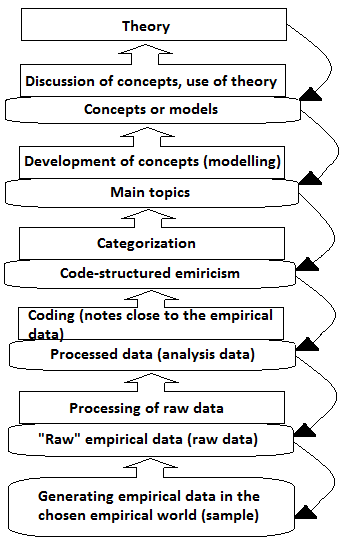
\includegraphics[scale=0.8]{sdi}
\caption[Stepwise deductive inductive method (SDI)]{Stepwise deductive inductive method (SDI) (modified from \cite{tjora})}
\label{fig:sdi}
\end{figure}

As a first step in this model there is data generation and processing of data. In this project we have by hand transcribed every detail from both audio and video recordings from both workshops. This forms the analysing data. We ended up with a huge amount of analysing data constituting for over 25 000 words from workshop 1 and about 6 000 words from workshop 2. The next step from here is coding of this data, which means to put empirical notes on interesting findings. The codes can be words and phrases describing interesting parts of the data material. The point is to try to reuse the codes if they fit to other parts of the findings, or to come up with new codes when new, interesting findings are discovered. After finishing through all the data material, you end up with a set of codes. The codes should only be developed from the empirical data, and not a priori, and it should be a natural link between the set of codes and the data material. In this project we did the coding by putting colors on the different areas in the material that had the same codes. From workshop 1 we handled the transcribed audio and video recordings equally and ended up with 88 codes. From workshop 2 we did the same, and ended up with 44 codes.

Usually, from a large data set you get too many codes to structure the data analysis properly. The next step is therefore to categorise the codes. This means to gather the relevant codes in groups. Here it is the research questions (problemstillingen) which lies in ground for what is relevant. The categories will usually be the main topics for the research's results. From workshop 1, we narrowed it down to 8 main topics, and this is the way we have presented the results in our report. This can be found in Chapter 11. From workshop 2, we ended up with 5 main topics, which are discussed in Chapter 14.

All the work that has been done up to this point has been done with the empirical data as a basis. The next step in the method is to develop concepts. Here theories will be more important. The categories, or main topics, that were developed in the last step, will now be related to theories about the topic. In this project we will set the categories up with the relevant topics discussed in earlier chapters, and use this to come up with a video game concept for elderly. Tjora \cite{tjora} distinguish between concepts and theories. He defines a theory like this (directly translated from Norwegian): "For a concept to have status as a theory, it has to be falsifiable and verifiable" \cite{tjora}. However, development of theories is not something that is done in all research, and it is quite common to use the concepts as legitimate results. In some type of research setting up the main topics or categories and discussion of these, can also be accepted as publishable results. This is what we have done in this study. 

\section{Quality of Research}
It is important to evaluate the quality of the research. As discussed earlier in this chapter we would want to maximize three criteria when doing research: generalizability, precision and realism. In our study we are trying to maximize realism, more than the other criteria. In addition there are other criteria that need to be considered when evaluating the quality of research. In \cite{tjora} Tjora discuss the three criteria: \emph{Reliability}, \emph{validity} and \emph{generalizability}. In addition, there are some possible pitfalls when doing qualitative research that needs to be acknowledged. We will discuss these elements in the next sections, and further discuss the quality of our research in Chapter Discussion.  

\subsection{Reliability}
It is important to distinguish between what is data from the research and what is the researcher's own analysis. By using direct citation the reliability of the research will be strengthened. How the informants have been chosen, and the relationship between the researcher and the informants, are important aspects for the reliability. Tjora also discuss the researcher's role in the study, which should idealistically be neutral. However this is impossible to maintain and it is therefore important to discuss how the researcher's position in the study can have an impact on the result \cite{tjora}.

\subsection{Validity}
"Is what we have found the answers to the questions we were actually trying to answer?", is a relevant question when evaluating the validity. In \cite{tjora} Tjora talks about communicative and pragmatic validity. The former gets tested with the research environment, where we relate the research to relevant theories and to previous studies done within the same topic. The latter can be tested with the question on if the research lead to changes or enhancements. The former is the one we primarily care about in the type of research we have done and other types of social science research. The validity will be even more strengthened by being open about how the research is performed and by explaining why certain data gathering methods have been used and the reasons for theoretical input. 

\subsection{Generalizability}
Some type of generalizability is a goal for most research. Tjora presents three kinds of generalizability within qualitative research \cite{tjora}: \emph{naturalistic generalizability}, \emph{moderate generalizability}, and \emph{conceptual generalizability}. The first one is when the researcher describes the details that has been done in the study so good that the reader of the study can self evaluate whether the findings are valid for the his or her own research. The second is about the researcher describing in what type of settings the findings will be valid. Examples of this can be at what time, at what places, in what context etc.. The last one, and also the one Tjora expresses his interest over, is about developing concepts, typologies, or theories that also can be relevant for other cases than the ones being studied. One of the reasons why Tjora has his interests in the last form for generalizing is because this relates to the goal of the SDI-model. In this study we have studied elderly's interactions with commercial video games with a goal of finding what aspects are important when developing a game for this user group. In addition we have studied their attitudes about exercising, and technology in general. The findings done in particular workshop 1, can be relevant also for others working with elderly and technology. Therefore, the third kind of generalizability is relevant in this study.


\subsection{Other quality aspects to consider}
In addition to the three main criteria Tjora also discusses the importance of transparency \cite{tjora}. The goal about this is that the readers should get   good enough insight into the research so that they can self evaluate the quality of the research. Thus, transparency is about presenting and discussing questions like for example how the research has been conducted, the different choices that have been made, what kind of problems that arose etc.. We will discuss this in Chapter Discussion.  In addition to the criteria presented by Tjora, we have looked into some issues discussed by Myers and Newman \cite{interview}. They summarize a set of possible pitfalls when doing qualitative research, and in particular when doing qualitative interviews \cite{interview}: \emph{artificiality of the interview}, \emph{lack of trust}, \emph{lack of time}, \emph{level of entry}, \emph{constructing knowledge}, \emph{ambiguity of language}, \emph{elite bias}, \emph{Hawthorne effects} and \emph{interviews can go wrong}. As the topics for our two focus group interviews were more about experience rather than knowledge, and because we did not experience any time pressure, we have evaluated most of these aspects to not have affected our data gathering. The only two of these aspects that might have affected out data gathering are \emph{elite bias} and \emph{Hawthorne effects}. The first is about how the interview can give incomplete and under-representative data  if only one type of group is interviewed, and that it therefore can be hard to understand the broader situation. Because of an overall time limit (the time allocated to the master thesis) and practical reasons, we only included one group of people with the same interests for learning and keeping up with technology. Our data gathering would probably be different, if we gathered a group of "random" people, because they would have different backgrounds and interests. The latter is, as briefly mentioned in Section 8.2.2, that people may behave differently when they are put in a specific setting with researchers interviewing or observing them. These two aspects will also be discussed in more detail in Chapter Discussion.


\section{Recruitment of Participants for the Workshops}
In this study we wanted to involve the relevant user group for the exergame. The relevant user group is senior males and females, aged 65 years and over. Because of time and practical limitations, we contacted an already established group, called "Seniornett". "Seniornett" is an organization in Norway which works to include the older generation (55 years +) in the emerging information technology and to help them gain digital competence. The organization was started in 1997 and is represented in every county in Norway.  Every semester the local clubs arrange 3-4 meetings with different topics related to technology, as well as an one-hour weekly meeting with technology assistance \cite{seniornett}. Even though this group includes seniors who are interested in learning about new technology, which is not common for every senior, we decided that this was a natural place to start recruiting for our workshop. This group may still have the same physical limitations, but may have a higher understanding of technology than other seniors. 

We contacted the manager of the club in Trondheim and briefed him about our project. He invited us to present the topic of our master thesis in their next meeting, which was 25. February 2013. This presentation would both serve as a contribution to this organisation, as well as a promotion of our project. The latter was mostly to gain interest in participating in the planned workshop. The presentation was mainly about the evolution of computer and video games from the beginning until today. As a part of this, we provided a presentation of serious games, and in particular exercise games. We also had a demonstration where we played Kinect Sports 2, shown on a big canvas. We played tennis with only one player, and showed them the possibility of multi-play by playing two players on the skiing game. Since the main topics for the presentation we held for "Seniornett" are not the main interest in this thesis, we will nor discuss the presentation any further. However, the presentation slides can be found in Appendix XXX for the interested reader. 

After the demonstration and the following discussion, we presented the planned workshop and invited the audience to help us with this. We told them that to make a user-friendly game, it is very important to involve the user, and that their help would mean a lot for our work on developing a game concept. We also explained what was expected from the participants in the workshop, and that this would be video- and audio recorded. In addition, we informed them that participating is voluntary and that the project is legally reported to \ac{nsd}. Everyone in the audience got a document containing information about the project and inform consent, see Appendix Y. Four people signed up at that time. 4 people signed up later by e-mail.

During and after the presentation the audience had some comments and questions. This feedback will be taken into account in our further work, but for convenience, we will discuss them together with the findings from workshop 1. 

\section{Execution of Workshop 1}
\label{sec:ws1}
We will now describe the set up and the execution of workshop 1. We will describe the purpose of the workshop, provide general information about participants, location and equipment, and present how the workshop was set up and performed. 

The primary goal for our first workshop was to introduce the participants, from now on called informants, to the Xbox Kinect technology and to three commercial games. We wanted to observe how they interacted with the technology and how well they enjoyed playing. In addition we had a focus group interview where the informants could talk about how they experienced the gaming session. We also used a short survey to get to know the informants' technology experience and attitude towards exercising.   

\subsection{General information}
The workshop was held over a two day period, the 13th and 14th of March, with location at "Gulhuset, Voll gård", a place familiar to the informants from "Seniornett". The workshop started around 2 pm and lasted approximately three hours. We had recruited eight informants from "Seniornett" to our workshop, three males and five females. They were divided into two groups, one for each day. One of the recruited females had an accident, which made it difficult for her to participate in the workshop. We therefore ended up with seven informants. The informants average age was 70.6 years (with a standard deviation of 7,9 years). In addition to us and the informants, we had two Ph.D. students with us the first day who acted in the role as facilitators. The second day our supervisor, Lill Kristiansen, joined us and took the role as the facilitator.   

In advance we had sat up an agenda for how we wanted to carry out the two workshop days,  see Table \ref{tab:agendaW1}.  

\begin{table} [ht!]
\centering
    \begin{tabular}{|l|l|}
       \hline
       \textbf{Introduction} & 15 minutes  \\ \hline
       \textbf{Survey} & 10 minutes  \\ \hline
       \textbf{Single play} & 15 minutes for each participant \\ \hline
       \textbf{Multi play} & 10 minutes for each participant \\ \hline
	   \textbf{Group discussion} & 65 minutes \\ \hline
    \end{tabular}
    \caption[Workshop Agenda]{Workshop agenda}
    \label{tab:agendaW1}
\end{table}  

\subsubsection{Location and Equipment}
We used "Gulhuset, Voll gård" as location for our workshop. This is a location well known for the informants. This location is used for various events, like theme lectures, song meetings, and story telling gatherings. This location has couches, tables and chairs, and it has a small kitchen where it is possible to make coffee and something to eat. "Gulhuset" was ideal to use for our workshop, not only because is is familiar to the informants, but because it was possible to make a living room-like atmosphere. It was also ideal because it is a place where we imagine that elderly could meet and play a future exercise game. At "Gulhuset" also possess a screen and a projector, which we used for our introduction. However, during the gaming session we chose to use a 46" Samsung flat screen. This was to make the gaming experience as natural as possible, as most people do not have screens and projectors in their own homes. We borrowed the flat screen from our department at NTNU. In addition to the the flat screen we had a Xbox, a Kinect sensor and three commercial games, which where use for the gaming session. This equipment was bought with support from a foundation for master thesis with computer science as subject [ENDRE litt på denne].   

In the workshop we used both video and audio recording to be able to interact with the informants. We rented a dictaphone, two video cameras (a Sony Handycam and a Panasonic 3MOS) and a rack for each camera. We wanted to use two video cameras to be able to make recordings from different angles. We had one video camera in the front of the room to capture movement and facial expressions, and we had one in the back to see movements from behind, in addition to recording interaction with the Kinect sensor and the games. The dictaphone was used for the group discussion.    

\subsection{Execution}
In the introduction we shortly presented ourselves and the background and main goal for our master thesis. We also informed about the purpose of the workshop, and presented the agenda for the day. The main part of the introduction was a review of the consent form, see Appendix X, where we highlighted important aspects as video and audio recording and that participation is voluntary. After the introduction the informants had some time to look over the consent form before they signed two copies, one for themselves and one for us. We then handed out a short survey to the informants, where they were asked a few questions about themselves, their technology experience and how they attitude are towards exercising. 

After finishing this session we started the gaming. The gaming session was divided into two parts, one part where the informants played some pre-chosen games individually, and one where they played together in pairs. The order of which part that where played first was for randomisation changed from day one to day two. In workshop day one there were only three informants, so they took turns playing during the multi player part. 

We presented the informants for three different pre-chosen commercial games, \emph{Fruit Ninja}, \emph{Your Shape Fitness Evolved 2012}, and \emph{Kinect Sports Season Two}. \emph{Fruit Ninja} is a game where you have to use your arms like a ninja to slice fruit that is thrown up into the air. The goal is to slice as much fruit as possible in a short period of time, without hitting any bombs that are thrown up together with the fruit. This games features simultaneous multi play with both competition and cooperation. The reason for using \emph{Fruit Ninja} in the workshop was to present the informants for a game based on pure fun and movement, with a concept far from something one might experience in real life. \emph{Your Shape Fitness Evolved 2012} is a popular exercise game for Kinect. This game has over 90 hours of activities, which can be used to design your own workout program. \emph{Your Shape Fitness Evolved 2012} follows your shape, fitness level and goals, and uses this to schedule the difficulty for the activities. You have the possibility to choose exercises for specific muscle groups, you can join classes like jump rope, cardio boxing and yoga, or you can take a virtual run in New York or Paris \cite{yourshape}. We chose this game to let the informants experience a game that are designed with exercise as the main purpose, with the use of realistic exercises. We presented a workout program for the informants that are designed specific for elderly. This program consist of a set of aerobic-like movements. \emph{Kinect Sports Season Two} is a game that consist of a bundle of six sports, which are tennis, darts, base ball, American football, skiing and golf. These sports stimulates movement and activity in a fun and motivating way, though exercise is not the main focus. \emph{Kinect Sports Season Two}, depending on the sport chosen, offers both competitive and cooperative multi play. We wanted to present this game for the elderly because of its amusing and real-life activities. \emph{Your Shape Fitness Evolved 2012} and tennis from \emph{Kinect Sports Season Two} was used for single play, while \emph{Fruit Ninja} and skiing from \emph{Kinect Sports Season Two} was used for multi play. 

Initially we wanted to start the play session without us helping the informants. We wanted to observe how well the informants understood the technology and the games presented for them. We believed that this would give us a more realistic result. We started out like this on day one of workshop 1 However, we experienced that the informants had problems understanding what they were suppose to do which lead to frustration and a bad experience. Therefore, after finishing the individual games, and before starting the multi player session, we explained how the Kinect sensor works and showed how to interact with the sensor. We also described the games they where about to play, and the goal of the games. On day two of workshop 1 we started with multi player and gave them the same introduction to the technology as before the multi player session on day one. On the games where they played individually, they went through the menu themselves on both day one and two. We guided them when necessary. 

When the informants had played individually and together in pairs we had a focus group interview. We asked them open questions about their experience of the technology and the gaming session. We wanted to know if they liked the games or not, and if so why. It was also in our interest to find out if this technology was something the informants would use, and if they could imagine using it for exercise. Our questions from our interview guide served just as a starting point for discussion, most of the time the informants talked freely with us and each other. The interview guide can be found in Appendix ..                 


\section{Execution of Workshop 2}
\label{sec:ws2}
We will now describe the set up and the execution of workshop 2. We will describe the purpose of the workshop, provide general information about participants, location and equipment, and present how the workshop was set up and performed. 

The aim of workshop 2 was to involve the target user group in the development process. We invited all the informants that participated in workshop 1 to a second workshop where we wanted to present our prototyped video game concept. The reason for inviting the informants to this second workshop was to get feedback on the prototypes, which is highly valuable when creating a user-friendly video game for elderly. This group of informants represents in this case the group of elderly that this game is targeted for, and are potentially future users of the system. They know know the interests and needs for this user group. In this workshop, we tried to give the informants an realistic impression of what an exercise game, based on their feedback, would look like. The way we presented the game was by prototypes made from PowerPoint and Photoshop. These are tools that were familiar to us, and it did not require any extra time to learn how to use them. Since we were in an early stage of the development process of a potential exergame, we focused on using low-cost prototypes.  

\subsection{General information}
Workshop 2 was held the 25th of April at "Gulhuset, Voll gård", the same location used for workshop 1. We met around 1 pm and started our presentation 20 minutes later. The total duration for workshop 2 was approximately two hours. We invited all the participants from workshop 1. Four informants chose to participate in workshop 2, in addition to the one women that was hindered to attend workshop 1 due to an accident. The group consisted of three men and two women. The informants average age was ... (with a standard deviation of ... years). We did not have any additional facilitators at this workshop. 

Beforehand, we had sat up this agenda:

\begin{itemize}
\renewcommand{\labelitemi}{$\bullet$}
\item Welcome.
\item Practical information.
\item Findings from workshop 1.
\item Presentation of our video game concept.
\item Feedback on our video game concept.
\item Presentation of our menu proposal.
\item Feedback our menu proposal.
\item Summary and finish.
\end{itemize}


\subsubsection{Location and Equipment}
We used the same premises as in workshop 1: "Gulhuset, Voll gård". 
For this presentation we only needed a laptop, a projector, and a screen. We used a private laptop, and the premises' screen and projector. Because of our desire to give our full attention to the presentation and discussion, we also video recorded this workshop. This was done with the use of a video camera, because we wanted to capture facial expressions in addition to the oral feedback. The video camera was a Panasonic 3MOS, and was borrowed from our department at NTNU. To make a cosy and comfortable atmosphere, we served cake and coffee.   

\subsection{Execution}
We started the presentation with an introduction, presenting ourselves, the goal of the workshop, and the agenda for the next hours. Some practical information about duration, the video recording, and requirements due to anonymity were also presented. The a short summary of workshop 1 was given, as well as the most important findings from this workshop. We did this both to fresh up the informants' memory, and to give the new informant a recap of workshop 1. This was also done to give the informants an idea of what we have focused on when creating our video game concept.        

In this workshop we alternated between presentation and discussion, so that there should not be too much information to remember for the informants. First, we presented the overall idea for the concept, before we proceeded with a more detailed description of the video game. The video game series was presented. We showed them prototypes of two different games from this series. We presented the games one by one, with an individual group discussion for each of them. To make it easier for the informants to comment and discuss we handed out pictures of the prototyped scenes (Sette inn figur/bilde av bilder på bord). 

We also presented for the informants the menu prototype we had made. We tried to present the menu in a way to make it look as realistic to a Kinect video game as possible. One of us stood in front of the screen simulating game play by pretending to "push the buttons", while the other controlled the PowerPoint presentation.  After the menu presentation we opened for a new, and final, group discussion. 

After the final group discussion was over, we took a few minutes to greet the informants, and thank them for their feedback, time, and participation.
 


\cleardoublepage
\chapter{Findings from Workshop 1}
In this chapter we will present our findings from workshop 1. The presented findings are based upon feedback and quotes from the informants, and our own observations during the workshop. The seven informants are referred to by using I1 to I7, and we have due to requirements to anonymity decided not to distinguish between male and female. Therefore, we refer to all the informants as females.  

\section{Perceived Usefulness and Value of Entertainment}
\emph{"Mostly, it was quite amusing"}. This was the general feedback from the informants after the gaming session. The informants were divided in their opinions about whether they would buy a game like this or not. Some of them would rather exercise for themselves or go to training centres, while others saw the gaming as more amusing than using a treadmill or an exercise bike. I5 stated that \emph{"I think this was very fun, so I would like to buy one of these. I have one of those exercise bikes in my basement, but it is so boring that I can not bear it"}.  Some of the informants stated that one of the reasons why it was fun playing was because it was a completely new experience. I6 said \emph{"Now I have been involved in something I have never been a part of before. [...] It is a new world that has opened up, that is for sure"}. Other reasons for why they enjoyed playing were that they could imagine playing with their grandchildren, and that it was a fun way to exercise. They liked the idea of combining gaming and activity. I4 said that \emph{"they [elderly] might think it would be fun to do this and be active at the same time"}. I6 explained that she felt different from when she was watching the other informants play, to when she was playing herself. \emph{"It gave more to participate that I had thought. Because, when I sat and watched it felt so unreal to have someone on the screen, but in the activity, when you got into it, it was not so stupid after all"}. The observations we did during the gaming session supports the feedback the informants gave us. There were a lot of smiling and laughing, and it seemed like they had fun.  

The informants liked some games better than others. The two games from Kinect Sports Season Two, tennis and skiing, were the game the informants liked the most. They thought the activities were fun and they liked the challenges the game provided. \emph{"I liked it very much. I like that kind of activity"}, was I4's general opinion about the games. The informants also liked that the game required something from them. About skiing, I3 said \emph{"This was a bit fun. Yes, it was. Because, here you have to pay attention and spend some effort [...]"}. I3 also liked tennis for the same reasons.  

Your Shape Fitness Evolved 2012, the personal trainer game, and Fruit Ninja were the two games that the informants liked the least. They did not see the need for the personal trainer game, as they rather would do these types of exercises in a training centre or by themselves. I3 said she did not like this game because it did not require anything from her. \emph{"The aerobic game I did not care for. That game anyone could do anywhere"}. However, when I1 chose which game she liked the most, she chose the personal trainer game as her favourite. This was because the other games had too much noise and loud sounds. Other aspects that were reasons for why the informants did not like a game were because the game did not present what you gained from doing the exercises, and it was hard to get points because of significant delay. 

When it came to Fruit Ninja, the informants did not see the usefulness of this game. They laughed a lot while playing, but they thought the game itself was stupid. I3 said \emph{I think it was stupid. It does not put any requirements on you. It was just.. [waving with his hands]"}. We did ask the informants if they thought the game was fun, even though it was a quite unrealistic game. I1 answered that \emph{"Yes, I think it was a bit fun. You see all the fruit that smashes. That was lovely"}. Even though some of the informants thought the game was fun, they did not see the point in playing it. One reason was that they did not see a connection between their movements and the outcomes on the screen. \emph{"You did not get any sense of whether you hit something or not"}. This was perceived as confusing, and they did not understand how to do things the right way. 

The informants said that if they were just going to do basic exercises, like in the personal trainer game, they would rather do this without a game. It was mentioned several times that they would rather go to their local traing centre and attend group sessions there. To want to use a game for exercising, it would need to contain a sport, or something else related to real life. \emph{"It would have been better to chop wood"}, I6 said after playing Fruit Ninja. Other possible game themes mentioned by the informants were swimming, rowing, picking apples, biathlon, interval exercises and a walk in the nature. \emph{"You mentioned apples. It might work to get it synchronised so that when you gather apples you can summarise the number. That might be a competition"}, said D4. One informant also suggested doing puzzle games on the map of Europe. In that way you could learn geography at the same time which would make the game more meaningful.

\section{Motivation and Mastery}

\emph{"Motivation is extremely important"}, was I5's opinion about playing games for exercising. Motivation was one of two things the informants mentioned as an important aspect for an exercise game. They told us that for elderly to use a video game for exercise, it has to possess features that will make them wanting to play. The informants stated goals and socialisation as motivational aspects for a game. Goals could be either achieving a high score, or just by moving their body to music.  \emph{"Moving to a rhythm, that is always positive."}, said I6. Social aspects of gaming was mentioned as important for the informants. I4 said that she felt that meeting others for exercising was motivating.   Another aspect that was considered as motivating was to get information about why they should play the game. The informants stated that if they could get to know, e.g. the training benefits, from doing the different activities, it would be more fun and motivating doing them. \emph{"We should get information about what [body parts] we are exercising when, and why we should do it. [...] I think that this [information] is very important for people as grown up as we are. We have to know why we should do this"}. 

One interesting observation we did during the gaming session was that the features in the games that were supposed to be motivating, were perceived as the opposite. Cheering, loud music, encouraging comments, fans and high scores were perceived as noisy and annoying, and not motivating at all by some, and was not noticed at all by others. \emph{"I became a bit irritated when there was a cute voice saying "yeah, that is great!", "hurrey!". I think it was stupid, I have to admit"}, said I1, while I3 said \emph{"I did not notice it at all"}. 

\emph{"Motivation and mastery. That is very significant"}. Mastery was also mentioned by the informants as a motivational factor. I6 said \emph{"It is all about the experience of mastery, which is essential. And the older people get, the more important it is"}. I6 emphasised how important the feeling of mastery is for elderly, in particular, because they would not continue doing something they do not master. The desire to master could lead to wanting to play the game over again. This is shown by I1's comment: \emph{"I think that I want to try it one more time. To master it [...]"}. When the informants first started playing the games, they were quite insecure and did not know how to perform the different activities and exercises. They completed the activities, but without the feeling of mastering it. But the informants did not see this as negative at all. They were all positive about it, and their common opinion was that it is all about training. \emph{"Nothing of this is difficult. It is just a matter of training"}, I3 said. 

While observing the informants interact with the technology, play the games, and walking through some of the menus, we saw that the informants mastered the different challenges better and better. They learned how to connect with the sensor, they quickly understood what was required from them in the various games, and they responded faster to feedback and information. This was both our observations and the informants own perception. When we asked them if they felt it was easier the second time they played, the majority of the informants answered \emph{"Yes"}. The informants stated that the feeling of mastery came fast, and that this was positive for the gaming experience. The first time information messages were shown on the screen, the majority of the informations did not respond to it. We had to assist them in what they were suppose to do. After playing for a while, they responded to the information messages without guidance, and they did it faster for each time. Some of the informants stated that they learned how they were suppose to play the game and how they should move to interact with the sensor by looking at the other informants play.  It was fun to watch how fast the informants learned.  

It seemed important for the informants to see a progress in the game, and that they are learning something. \emph{"I believe in games that have the characteristic of play and that you can see that you get better"}, I2 said. This will provide the players with something useful, that will make them want to play again.

As a part of mastery it was also mentioned that we need to consider all the different groups of elderly to make suitable tasks for everyone to master. One of the informants mentioned different groups to keep in mind: "the people who already have decided to keep their body in shape", "people who wants to know if they are doing the exercises right", and "the people who are already inactive". For the latter group she mentioned the importance of getting help, e.g. from grandchildren.  Another group mentioned are the people who can not stand or walk, who might be sitting in a wheelchair

\section{Immersion and Engagement}
The informants showed a lot of engagement and different feelings during the gaming session. They immersed into to game, and gave it all to complete the different challenges. In most of the games the informants used body movements eagerly. The informants also burst out with various comments like \emph{"yes yes yes yes"}, \emph{"noooooo"} and \emph{"ooh, I wanted that pineapple!"}, while playing. In addition, the informants laughed a lot during game play. A few of the informants only used monotonous movements, like just waving their arms up and down with not that much engagement.  

Not all the games created feelings of immersion and engagement. The personal trainer game was a game that the informants "just did", without showing any particular emotions. There were not many comments during game play, and there were no laughter or engagement. We only observed concentrated faces. However, the informants tried their best, and most of them went through the exercises with controlled and powerful movements, in tempo with good rhythm.       

The informants expressed that they felt, in some of the games, that there were a lot going on at the same time. We asked them if they felt it was easy to focus on the challenges, exercises and activities, although there were a lot of hustle. The informants agreed on that while playing, they were totally focused. I7 said \emph{"When you are in the game, then you do not see the outside world, then you are concentrated"}. The informants stated that they lived into the character of the avatar. They did not feel that the avatar was a person separate from themselves. \emph{"I felt like the person [avatar] itself"}, I3 said. 

\section{Functionality and Usability}
\subsection{Introduction and instructions}
It was a common opinion that the different games should spend more time on instructions and explanations on the different exercises. \emph{"It needs to be a softer and more instructive introduction into the game's rules"}, I5 said. Especially in the personal trainer game, this was the case. I1 compared this to the way they did it in an aerobic class she used to attend in her younger days. She explained how they practised the exercise slowly before they could do it fast. The personal trainer game started up quickly, with no room for practice or warm up, and it held a high tempo. The informants did not know how to do the required movements, as no information where given. Most of the informants got the movements after a few steps, as they recognised the exercises from aerobic classes at their training centres. After playing, most of them agreed that the exercises were OK and that it was only a question of learning. 

All the informants could agree that there were some positive health effects, however, they did not exactly know what they were exercising. They urged that the games should include information about which body parts they are exercising when they are doing the different tasks. Another general opinion was that they wanted to know if they were doing the exercises right or not when they were playing.

When the informants played their first game, they seemed confused and unknowing. One informant started pointing on the screen and asked \emph{"How do I point?"}, meaning how she could press the buttons. When playing the personal trainer game I1 asked \emph{"Press the button? Is there any button here?"}. It was clear that it was not obvious what was meant by pressing a non-physical button. None of the informants had ever played games like these, and did not understand how the game could be controlled by their body movements, even though we had explained this. 

\subsection{Complicated menus}
There was a common agreement that the games had too complicated menus.  The avatar hand that was navigating on the screen was too sensitive, and it was hard to keep the hand still long enough to actually "press the button". In the sports game buttons were pressed by holding the hand over the button for a certain amount of time. \emph{"This is worse than working with a mouse [on the computer]"}, I6 said. The time needed to hold over the different buttons seemed to be too long. In the personal trainer game the avatar hand was, in addition to being too sensitive, unclear and at times almost invisible. It did not really look like a hand. This seemed to cause some problems because not all informants understood that the object on the screen was their hand. Two informants suggested that an arrow-marker like the one used on most computers would be more intuitive and easy to use. 

\emph{"The menu was extremely difficult [...]"}. In the same game, the menu appeared to be very complicated, as a result of being big, complex and sensitive. This made it difficult to know where to go, as well as to push the right buttons. There were a great amount of information on the screen, which made it difficult to choose the right alternative. Three informants was challenged to go through the whole menu, and they, especially, struggled a lot. To navigate between the pages in the menu, there where arrows on the sides that should be pressed. These arrows were hard to see, and they were very sensitive. When telling the informants to scroll through the menu by pressing the right arrow, I1 said \emph{"Which arrow?"}. In addition, this menu had a huge "back"-button that the informants pressed several times without intention. 

Also with Fruit Ninja the informants had problems with the menu. The menu was crowded with elements, which made it hard to hit the correct buttons. In addition, the menu made it difficult for the informants to distinguish between the menu and the actual game. I6 and I7, who were playing together, stood in the background and waved their arms towards the screen while we tried to go through the menu and start up the game. 

\subsection{Information and feedback}
There were various perceptions of the information and feedback given during game play. Some of the informants were not affect by the information given, and at times they did not even recognise its presence. \emph{"I did not react to the text at all. If you had asked me, I would not know it had been text"}. I5, on the other hand, felt that there was too much information at the same time, which made it hard to concentrate. \emph{"No, I think you should limit the total amount of information"}.  I2 said she had seen the text but it disappeared too fast, so she did not have the time to read it all. She suggested that it should be a way to confirm that you have read the information before it disappears. 

We observed that at least one informant spent some time reading the text in the menus in the personal trainer game and in the tennis game. At one point the informant had to move closer to the TV-screen to read the text. This might be an indication of too small text in these menus. 

Most of the informants agreed that it was too much unnecessary information. However, it seemed that it was desirable with feedback on what they were doing. \emph{"I think it is very nice to see how far I have walked, and how fast I have walked, and how much downhill and uphill and things like that"}, I1 said, referring to a mobile application she was using to give her information about her progress when cross-country skiing. This implies that feedback on their progress is important for some of them.  

The instructions in both the tennis and skiing game, like "raise hand above head to play" or "move closer to the sensor" were well understood by almost all informants. However, we had to assist some of the informants a couple of times by reading the message given on the screen. 

Not all informants understood that there were introduction videos and instructions in the beginning of the game. This became clear to us as most of the informants tried to do what the avatars did in the video, and seemed confused when nothing happened. \emph{"Should I try to hit it [the ball]? What am I suppose to do now?"}, I1 asked during the introduction video. However, it appeared that the second instruction video that was shown between two matches in tennis, was understood as an introduction video, and that they all learned from it. However, when the game was finished, some of the informants did not understand that the game was over. Especially did this apply for the tennis game, where most of the informants ended up just looking at the screen.   

\subsection{Graphics and sound}

We asked the informants about their opinions about the music in the games, and I1 answered \emph{"I think everything about that was too much"}. I2 replied with \emph{"I like Mozart better"}. On other type of music that was mentioned as more suitable than ordinary pop music was music with swing rhythms. All the informants agreed that music is important to keep the rhythm when exercising, but that they would prefer the music not being too noisy. It was also a general opinion that the music was inappropriate.  I7 said \emph{"You get sensitive [to sound]. You do not want it. You want it quite. You would want to be active, but without too much background noise"}. I4 added \emph{"[...] I would prefer walking out in the nature. Then you can listen to the birds [...]"}.

It was a general opinion that there were too much elements on the screen during game play. I7 stated this by saying \emph{"It is too much elements on the screen. Where should you look?"}. Some of the informants also felt it was too much going on at the same time during game play, and I5 suggested that there could be different levels of things that happens in the game. \emph{"[...] Eventually when you get better and manage to keep track of more things, you can add more things [to the game] that happens. A lot of what happens in these games are not relevant"}. 

On the question about what they thought about the avatars and the picture in general, I5 answered \emph{"I think it was very confusing to see myself. Especially to see both of us [herself and the trainer in the game] [...]"}. In addition, most informants agreed that the avatar of themselves in the personal trainer game made them look fat, which they did not like.

\subsection{Technological issues}

\emph{"It bothered me that I did not see the correlation or the relationship between my own body movements and what was happening on the screen"}, I2 said about the gaming experience. All of the informants complained about the delay that was present in the games. This applied for all the games but Fruit Ninja, and it was mentioned as a problem several times. The delay made it hard to move correctly and in time. For example several of the informants had problems passing through the gates and to perform a perfect jump in the skiing game because of the delay. \emph{"Missed the jump? I jumped so quickly. That is just nonsenses"}. The delay in the games made it difficult to get points and achieve high scores, which again gave the informants the feeling of not mastering the movements. \emph{"I think my movements on the screen look too slow. Are they that slow?"}, I6 asked while playing. 

The technological aspects of the games became a source of confusion for most of the informants. \emph{"There were some small technical details that were problematic. [...] I could not see in the skiing game that anything special happened with me. [...] And in tennis, it was something about the time aspect, with when you tried to hit and when you actually hit [the ball]. I got a feeling that they [the game] helped me a lot in the beginning"}. This problem occurred for example when in the tennis game when the informants tried to coordinate the one hand with the racket and the other hand with the ball. The delay made it difficult for the informants to see when they actually hit the ball. Some of the informants expressed that the significant delay interfered with the gaming experience. I5 said that \emph{"I experienced the tennis and skiing game as games with lack of technical perfection. It was not good enough technically to make a real time experience"}. However, I5 said that if they got used to the delay, they might have more fun.

Most of the informants had a hard time coordinating their moves in the personal trainer game, as the movements were quite fast. Some of the movement were for many difficult to perform correctly. I6 commented that it was all about training, and that they would master it after getting familiar with the game. I5 answered to this with \emph{"Sure, but it is possible to make it less confusing"}. I1 replied that she rather would exercise without the game. The informants also experienced similar problems with the tennis game. The ball came quickly, and it was difficult to coordinate the hand fast enough. This applied especially when the ball came on the opposite side of the body from where the racket was held. One of the informants ended up trying to hit the ball with her left hand, even though she had the racket in her right hand. 

After playing Fruit Ninja I7 told us that she had trouble understanding how she could see where she hit the fruit. It also seemed that I1 did not understand what actions did cut the fruit in half, she just stood there and waved her arms while she looked quite confused. \emph{"It is just to wave your arms. There is no system"}, said D3, implying that the game did not require anything from them. In addition, they did not see the relationship between what they did and what they achieved. \emph{"[...] I did not get any feedback on my movements"}, I2 said. 

\emph{"The game that required something from you was the skiing game. The rest of the games did not require you to follow the instructor apparently"}, I3 answered after being asked how they experienced the games. It was apparent that some of the informants did not understand what they were meant to do in the games and that they just "did something". 

Some informants mentioned that the skiing game was very fast. At the same time there was a comment about the importance of having the fast pace, to make the game exciting and fun. There was one situation in the skiing game that especially seemed to cause confusion and frustration. When playing multi player, there were two matches, where the players in the second match would have to switch tracks. The informants had troubles understanding which track that was their track and had comments like \emph{"Eh.. I do not understand"} and \emph{"Are we going in the same lane?"}. I5 was confused while playing, \emph{"First red and then blue and then blue and then.. [...] This does not work"}. The fun and enjoyment we observed the first round of skiing was the second round replaced with frustration. 

\section{Physical Outcome}

The informants had a general opinion that all movements are good for your body, and that these games required you to move in a good way. They had comments like \emph{"If it [the game] is good for your body? Yes it is. All kind of movements are of the good"}, \emph{"You get warm"}, \emph{"[...] I felt it was useful, in a health-related way"}, and \emph{"It was amazing how much body you actually used on so little"}. However, there was mentioned that if the aim of the game was exercising, it should be build on the whole range of exercising, from warm-up to stretching. 

In tennis and Fruit Ninja, several of the informants mentioned that their shoulder and arm were in pain after playing. In tennis, the player only uses one arm, and the workload gets asymmetrical.  
    
\section{Playing Together}
\emph{"I think skiing was fun. But I am thinking it would be more fun top play with a grandchild in a suitable age. Then I could say "should you and grandma play the ski-game together? Just for fun?""}, I5 said about the social aspects of the different games. She continued with \emph{"I am thinking that in a nursing home we would probably like to play with someone"}. Some of the informants were clear in their opinion about whether they would play alone or with others, and I7 stated that \emph{"[...] I do not want to do this alone at home"}. I4 said she  enjoyed playing alone, \emph{"I think both [playing alone and together] was OK. [...] I believe in  exercising in small groups"}.

A general opinion was that this game could suit well in a nursing home setting, in a small group setting, or as an activity to do with grandchildren. It seemed that most informants liked to play together, however some informants mentioned that they were indifferent. They enjoyed playing together in the games that were made for fun and entertainment, like skiing and tennis, while with games meant for exercising, like the personal trainer game, they felt it would be better to do alone. One informant told about her mother in law that got inactive on her last years. She believed that the only way to encourage her to become more active by playing games would be if there were some social aspects within the game, like playing together with a grandchild. 

Everyone agreed that being social and meeting people are important parts in life, but that they would do it on their own time, and not be locked to a specific group or time. I5 felt that meeting together in a group for exercise would give her a sense of pressure that she does not like. \emph{"[...] I have had pressure all my life. I do not want it anymore. I do not want to put myself in that situation where people come and ask "are you going to join this?""}. I7 agreed that this type of pressure is not motivating. \emph{"It is like this: well-being is attractive, pressure is not attractive"}, I6 said, referring to the importance of doing things voluntarily. However, just having the opportunity to go out and meet people, like in an arranged training group, seemed to be important for all of the informants. 

\emph{"You are talented"}, and \emph{"You are starting to get it now"}, are examples of comments the "audience" told their co-informants while they watched the other informants play. They encouraged each other, and provided positive and motivating messages. The informants that were playing seemed to enjoy this feedback. This feedback made the gaming session more social and fun.  

We asked the informants if the could imagine themselves playing at home in their own living room, and competing with friends over the Internet. This they were not very positive about, and it seemed like they did not understand what we meant. \emph{"This is very distant for me"}, was I6's comment. \emph{"It would probably be more motivating to just ask her if she wanted to come over and play"}. These answers show how being social over Internet is quite unfamiliar to the informants. To make a game like this social, all the informants agreed that meeting in person would be better. On the other hand, the informants using this training mobile application, seemed to like to share exercise information with friends.

\emph{"[...] If there is going to be any point in doing something together, it needs to be that you are enhancing each other. Like that you get a better result if you are cooperating. [...]"}, I5 said. She had a strong meaning about how to play together, and meant that it was more motivating to cooperate rather than compete. The other informants seemed to be indifferent whether they were competing or collaborating.

\section{Experience and Understanding of Technology}
None of the informants had used a technology like Xbox Kinect before, and they all said that it was a completely new experience for them. I3 said \emph{"I have practically never seen it before"}. In fact, the informants said that they never had used any kind of video game technology. \emph{"Waste of time"}, I5 said, \emph{"I could never have time for something like that"}.  

The informants generally showed interest in the technology and our project during the workshop. They asked about the EU-project, where the games were made, and how much the Xbox Kinect costs. The informants showed interest in what equipment needed for them to play at home. \emph{"Does it connect to a TV?"}. I7 commented that it is important that the technology is easy to install. The informants were also eager to ask questions about the games, where this was related to information given, their own performance, difficulty levels and confusion. While looking at two informants playing Fruit Ninja I7 had questions as \emph{"Can you steal others fruit when you play?" and "What do you lose points for?"} 

During the group conversation there were questions about our work. They wanted to know how we would proceed from that point, and what we imagined as our result. One informant also asked the facilitators that joined us the first day about their role in this project. When we were about to finish the group conversation, I6 asked \emph{"[...] What we are telling you, is it usable? Can you use if for something?"}. We answered that their feedback through the workshop is highly valuable, and that it will be used as a basis for the video game concept in our master thesis. I3 complimented our work with \emph{"It is admirable what you are working with this, that I have to say"}. 






\cleardoublepage
\chapter{Concept for an Exergame for Elderly}
\label{chap:concept}
This chapter is about the second and third activity in the cycle of user centered design, specifying requirements and producing design solutions, see Figure \ref{userdesign}. Based on findings from workshop 1 and from theory presented in earlier chapters, we have created system requirements and designed a concept for an exergame for elderly. The exergame concept will from now be called the exergame or the game. The exergame focuses on including movement and exercise in real-life and well-known activities. This will be provided in an entertaining and motivating way. We will present the requirements this exergame is built upon, before we describe the exergame in more detail. This will include games and challenges, the exercises used, goals, obstacles, and how to achieve points. In addition to the exergame, we have also, based on a course in \ac{hci} at NTNU, and guidelines for developing interfaces for elderly, designed a menu for the exergame. 

The exergame will be presented based on theory about designing video games, as discussed in Chapter \ref{chap:vg}, and can serve as a part of a design document, according to what is described in Section \ref{sec:designphase}. We acknowledge that not all the elements that should be included in a design document are present in this chapter.

When creating the exergame, our prime focus has been on the intended user group. The game is based upon the requirement specification, presented in Section \ref{sec:req}. In addition to this, expressed thoughts and opinions from the informants during workshop 1 are emphasised. The figures in this chapter are prototypes presenting what the exergame will look like. We will use these prototypes to present the idea of the exergame and design for elderly in a second workshop, and we have therefore focused on making prototypes that gives the users a realistic impression of the final result. The prototypes are medium-fidelity prototypes, made with software tools such as PowerPoint and Photoshop. The prototypes presented in this chapter will be in English, to be in accordance with the language this report is written in. The original prototypes are in Norwegian and can be found in Appendix C and D. 

We will start by presenting the system requirements in Section \ref{sec:req}, before we continue with describing our exergame with its story and included elements. Various scenarios will be presented with the use of medium-fidelity prototypes in Section \ref{sec:outinthenature}. Functional design, presented in Section \ref{sec:functionaldesign}, will give a concrete representation of one possible level of each of the proposed games. Design and description of the menu for the exergame are presented in Section \ref{sec:menu}. This chapter can serve as a part of a design document that can be used by developers to understand and design this exergame.  

\section{Requirements}
\label{sec:req}
We have set up a list of requirements for the exergame, which specifies what the system shall do, and which constraints the system shall hold. The requirements have been developed with foundation in all theory presented in the earlier chapters, as well as findings from workshop 1. We have written requirements according to what we have presented about requirement specification in Section \ref{sec:fourpillarsofdesign}, and they are therefore divided into functional and non-functional requirements. In the exergame we have mostly focused on the functional requirements, and interface requirements, which is a subsection of non-functional requirements. 

We will support our requirement specification by referring to relevant references, findings from workshop 1 (referred to as fw1), motivational factors from Section \ref{subsec:motivator} (referred to as m.x), and guidelines listed in Section \ref{sec:summaryguidelines} and Section \ref{subsec:golden} (referred to as g.x or e.x respectively). These will be listed in the rightmost column. It is important to acknowledge that the requirements also are based upon our own ideas, thoughts and opinions. 

\subsection{Functional Requirements}
The functional requirements in Tables \ref{tab:func1}, \ref{tab:func2} and \ref{tab:func3} present the services and functionality the exergame shall offer.

\begin{minipage}{12 cm}
\begin{table} [H]
\centering
\begin{tabular}{|>{\raggedright}p{0,7cm}|p{8,8cm}|p{1,5cm}|}
\hline
\textbf{No.} & \textbf{Requirement} &  \textbf{Ref.}\\ \hline
1.1 & The system shall be an exergame that emphasises exercise and physical movement. & \cite{project} \\ \hline
1.2 & The system shall have a fun and entertaining story with focus on game play.  & \cite{project} \cite{zyda2005visual} \\ \hline
1.3 & Exercise shall be subordinate to the story. & \cite{zyda2005visual} \\ \hline
1.4 & The system shall meet the diversity in people. & g.8, e.2, m.11, fw1 \\ \hline
1.5 & The system shall provide natural and familiar surroundings and elements. & g.9, fw1\\ \hline
1.6 & The system shall provide natural and familiar activities, challenges, and exercises. & g.9 \\ \hline
1.7 & The system shall provide both physical and cognitive challenges. & m.8, fw1 \\ \hline
1.8 & The system shall allow for decision making before and during the game. & \cite{understandingvg}, m.9 \\ \hline
1.9 & The system shall provide players with clear instructions on how to use and interact with the game. & g.5, e.8, fw1 \\ \hline
1.10 & The system shall provide players with clear instructions on how to perform various activities, challenges, and exercises. & \cite{sweetser}, \cite{project}, g.5, g.6, e.8, m.2, fw1\\ \hline
1.11 & Instructions shall include information about the health benefit gained from playing. & m.3, fw1\\ \hline
1.12 & Instructions shall be given during game play when appropriate. This shall be done to avoid the need to memorise information. & \cite{sweetser}, g.5, e.8 \\ \hline
    \end{tabular}
    \caption[Functional requirements, part 1]{Functional requirements \footnote{g - guidelines, e - guidelines from the Eight Golden Rules, m - motivators, fw1 - findings from workshop 1}}
    \label{tab:func1}
\end{table} 
\end{minipage}

\begin{minipage}{12 cm}
\begin{table} [H]
\centering
\begin{tabular}{|>{\raggedright}p{0,7cm}|p{8,6cm}|p{1,7cm}|}
\hline
\textbf{No.} & \textbf{Requirement} & \textbf{Ref.} \\ \hline
1.13 & The system shall give players the time they need to read instructions. & o.23, m.9, fw1 \\ \hline 
1.14 & The system shall allow players to skip instructions. & \cite{sweetser} e.7, m.9, fw1 \\ \hline 
1.15 & Player shall be given feedback on their actions. &  \cite{sweetser}, e.3 \\ \hline
1.16 & Feedback given shall be positive and motivating. &  \cite{sweetser}, \cite{project}, g.6 \\ \hline
1.17 & Feedback shall only be given when appropriate. Interruptive feedback shall be avoided during game play. &  \cite{sweetser}, fw1 \\ \hline
1.18 & The system shall be a progression game. & \cite{understandingvg} \cite{sweetser}, g.15 \\ \hline
1.19 & The system shall have small subtasks with clear goals. &  \cite{sweetser} \cite{john2012smartsenior}, g.15, m.6 fw1\\ \hline
1.20 & Player shall be informed about progression and results. & \cite{sweetser} \cite{john2012smartsenior}, e.3, m.7, fw1 \\ \hline
1.21 & The system shall allow multi-play. & g.10, m.9-11, fw1 \\ \hline
1.22 & Multi-play shall have the possibility to be performed both as collaboration and competition. & \cite{sweetser}, fw1\\ \hline
1.23 & Player shall be given the possibility to choose preferred difficulty level. & \cite{sweetser}, g.15, g.16, m.9, m.11, fw1\\ \hline
1.24 & The system shall allow for players to choose individual difficult levels. & \cite{sweetser}, g.16, m.9, m.11, fw1\\ \hline
1.25 & The system shall be able to adjust difficulty level after players' progression. & \cite{sweetser}, fw1 \\ \hline
    \end{tabular}
    \caption[Functional requirements, part 2]{Functional requirements \footnote{g - guidelines, e - guidelines from the Eight Golden Rules, m - motivators, fw1 - findings from workshop 1}}
    \label{tab:func2}
\end{table} 
\end{minipage}

\begin{minipage}{12 cm}
\begin{table} [H]
\centering
\begin{tabular}{|>{\raggedright}p{0,7cm}|p{8,6cm}|p{1,7cm}|}
\hline
\textbf{No.} & \textbf{Requirement} & \textbf{Ref.} \\ \hline
1.26 & Activities provided by the system shall include exercises for all muscle groups. & \cite{guidelines} \\ \hline
1.27 & Exercises used shall be proved to be good for training for elderly. & \cite{project} \cite{john2012smartsenior}\\ \hline
1.28 & Activities shall be possible to perform both sitting and standing. & g.17, m.9, m.11 \\ \hline
1.29 & Player shall be given the possibility to choose gender on their player character. &  g.8, g.12, m.9, m.11 \\ \hline
1.30 & The system shall always provide players with the possibility to reverse their actions. & o.25, e.6, m.9 \\ \hline
1.31 & The system shall create a user profile where players' progression and results can be saved. & \cite{project} \cite{john2012smartsenior} \\ \hline
1.32 & The system shall provide players the possibility to share their profile, or part of their profile, with friends. &  \cite{sweetser} \\ \hline
1.33 & The system shall be able to be used as a tool for physiotherapists. & \cite{project} \cite{john2012smartsenior}\\ \hline
1.34 & The system shall give physiotherapists the possibility to set parameters to customise the exergame for each individual patient. & \cite{project}, \cite{john2012smartsenior}, g.1, g.33  \\ \hline
1.35 & The system shall give physiotherapists access to players'/patients' profiles. & \cite{project} \cite{john2012smartsenior}\\ \hline  
\end{tabular}
\caption[Functional requirements, part 3]{Functional requirements \footnote{g - guidelines, e - guidelines from the Eight Golden Rules, m - motivators, fw1 - findings from workshop 1}}
\label{tab:func3}
\end{table} 
\end{minipage}


These requirements will be used as a foundation for the exergame, and they will serve as input to the functional design presented in Section \ref{sec:functionaldesign}. Requirement 1.33 - 35 focus on the physiotherapists view of the system. As previously mentioned, we have in this thesis emphasised interface design for the end users which are elderly people. However, it is important that these three requirements are included in future work on the exergame. This is because we in our previous project \cite{project} evaluated physiotherapists to be the proper customer for the game. We believe that in today's market the game will not experience success going straight to the end users \cite{project}.  

\subsection{Non-Functional Requirements}
The non-functional requirements presented in Table \ref{tab:nfunc1} and \ref{tab:nonfunc2} describe constraints to follow for the exergame to ensure good usability in terms of interface design.

\begin{table} [H]
\centering
\begin{tabular}{|>{\raggedright}p{0,7cm}|p{8,4cm}|p{1,9cm}|} 
\hline
\textbf{No.} & \textbf{Requirement} & \textbf{Ref.} \\ \hline
2.1 & The system shall provide good graphics in 3D, which makes the game world look real. & \cite{understandingvg} \cite{john2012smartsenior}\\ \hline
2.2 & The system shall use a character to portray the player. & \cite{understandingvg} \cite{john2012smartsenior}\\ \hline
2.3 & The system shall provide sound and music appropriate for the user group. & g.8, fw1 \\ \hline
2.4 & The system shall provide sound and music appropriate for the game theme and the intensity in the current activity. & \cite{umlapproach}, m.13, fw1 \\ \hline
2.5 & The system shall have a menu, which is used by the player to make choices about game play. & \cite{gerling2} \cite{john2012smartsenior}\\ \hline
2.6 & The menu shall be clear, simple, and intuitive. & \cite{sweetser} g.4, o.8, e.8 fw1 \\ \hline
2.7 & The menu shall be consistent. & o.9, e.1 \\ \hline
2.8 & Menu buttons shall not be too sensitive. & fw1 \\ \hline
2.9 & Menu buttons requires "push" to perform any action. &  fw1\\ \hline
2.10 & The navigator shall not bee too sensitive. & fw1\\ \hline
2.11 & The navigator shall be clear. &  fw1\\ \hline
2.12 & Information shall be easy to see, and understand. & o.24, o.25, e.8\\ \hline
2.13 & Information shall be written in a familiar language with everyday words. & o.7\\ \hline
\end{tabular}
\caption[Non-functional requirements, part 1]{Non-functional requirements, interface requirements}
\label{tab:nfunc1}
\end{table} 
\begin{table} [H]
\centering
\begin{tabular}{|>{\raggedright}p{0,7cm}|p{8,4cm}|p{1,9cm}|} 
\hline
2.14 & Information shall be written with an easy-to-read font in an appropriate size. &  g.2, o.1-5\\ \hline
2.15 & There shall be clear contrast between background color and text color. & g.3, o.14-20 \\ \hline
2.16 & Elements that are essential to the game shall stand out. & g.4, o.8, o.20\\ \hline
2.17 & The system shall avoid using elements that are unnecessary for current situation.  & \cite{sweetser}, fw1\\ \hline
\end{tabular}
\caption[Non-functional requirements, part 2]{Non-functional requirements, interface requirements}
\label{tab:nonfunc2}
\end{table} 

\section{The Overall Story Line}
\label{sec:outinthenature}
We will now present the story line of the exergame. This will be based on the requirements provided in the tables above. We will refer to the relevant requirement with [req. no] throughout the presentation. 

"Out in the nature" ("Ut i naturen" in Norwegian) is the title of our exergame. This is a game based on a forest theme and it consists of real-life activities that are familiar to most people [req. 1.5]. The different activities are natural to find and do in the forest or in the nature, hence the game name. The goal is to experience beautiful nature while playing, and at the same time exercise and achieve physical activity[req. 1.3-4]. Bringing the beautiful nature "to life" is achieved by giving the game a 3-dimensional representation [req. 2.1]. The exergame consists of five individual games, one longer, compounded game that will engage the whole body, and four, shorter single games with various challenges and exercises, both for the mind and body [req. 1.7, 1.26].        

We have used familiar elements that can be found in the forest, like rocks, creeks, and logs. When we have chosen to use other elements, these are well-known, and easy to relate to for the elderly [req. 1.5]. One example of this is hearts and their relation to health. In addition, our intention has been to avoid unnecessary details that can lead to confusion and distraction [req. 2.17], in accordance with simplistic design, discussed in Section \ref{sec:simplicity}. Music and sound effects in the game will be natural when possible [req. 2.4], like birds twittering and the wind in the trees. The informants mentioned that classical music, e.g. Mozart, would be more suitable than the pop, computer-made music that was used in the commercial games we presented for them [req. 2.3]. An idea can therefore be to use classical music that will fit a walk in the beautiful nature a warm summer day. When there are challenges and activities that requires intensity, the idea is to use music with a rhythm, without being noisy [req. 2.4]. We will not present any specific music examples suitable for this exergame, since that is outside our area of competence. 

The player will be presented in the game as a character with "real-life" features. As described in Section \ref{subsub:fictionalworld}, the player character can be described by three different categories: avatars, actors and role playing. From the definition, the player character here will be an actor. However, in commercial Kinect games the player character is called an avatar, and we will therefore do the same. They do not have a distinct personality except from being a "a normal human being", but they are well integrated into the story. We will use two different male and female avatars [req. 1.3, 1.29], this to meet with the requirement of having two simultaneously players [req. 1.21]. All characters are dressed in training outfits, females in training leggings and t-shirt, and males in long pants and t-shirt. The different characters will have different colors on their t-shirts to make it easy for the players to distinguish between them. The male avatars have either blue or green t-shirts, while the female avatars have either yellow or pink t-shirts. The males have short hair, and the female have half-long hair. For convenience, the characters will have international names, like Anne, Eva, Charles and David. The avatars will be seen in a third-person perspective. This is because it is important for the player to see the avatar of herself to see if she is doing the exercises correctly. 

"Out in the nature" is meant to be an exergame for elderly, but it is important to not just focus on the exercise. This exergame has an entertaining and motivating story that is the main focus in the game. The exercises are only subordinate to the story [req. 1.1-3]. However, we will include the opportunity for the player to choose which part of their body they want to exercise. In the first step in the menu, the player is given the choice of how she wants to play, see Figure \ref{fig:menuStart}. The player can choose between the compounded game, choosing to play based on exercising a preferred muscle group, or the player can choose among the four single games [req. 1.8]. Our choice of including this in the exergame is based upon feedback from workshop 1, where the informants stated that it was important to make own decisions on how, and when, they would like to work out.                     

\begin{figure} [H]
\centering
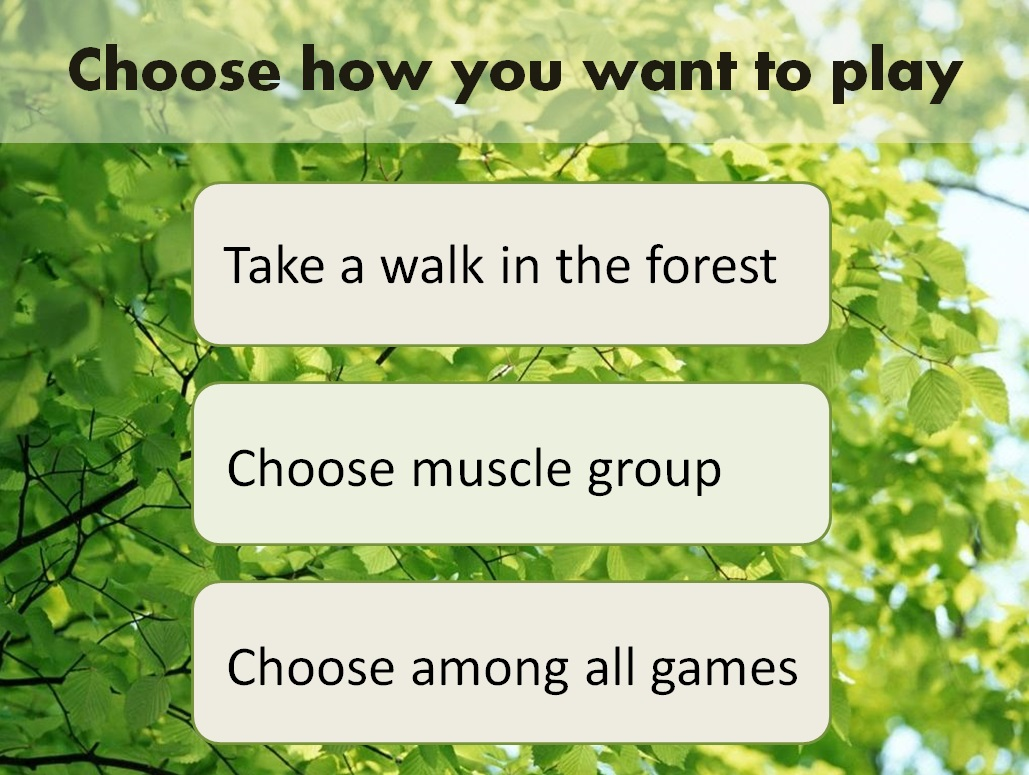
\includegraphics[scale=0.24]{choosePlay.jpg}
\caption[The menu - start]{In the first menu step, the player is given the opportunity to choose how they would like to play. The can go for the compounded game, play according to a chosen muscle group, or they can choose among the four single games.}
\label{fig:menuStart}
\end{figure} 

\subsection{Exercises}
The activities we have selected for our exergame are based upon findings from workshop 1, and our own ideas, but the main reason for using these activities is because they involve exercises that have been proved to be good for elderly [req. 1.27]. In Section \ref{sec:summaryguidelines}, stepping, balance and strengthening exercises are proposed as suitable for elderly. This was also suggested as appropriate exercises by The Norwegian Directorate of Health \cite{aktivitetsbok}. In addition, we have used \emph{Øvelsesbanken} \cite{eldretrening}, which is presented in Chapter \ref{chap:olderexercise}, as a guide to find exercises to use in our exergame. We have picked out 18 exercises from \emph{Øvelsesbanken} that we argue are a good foundation for the exergame. Some exercises chosen are "picking apples", see Figure \ref{pickingapples}, "walking", and "rowing". All the chosen exercises are presented in Appendix B. Most of the exercises have the possibility to be performed both sitting and standing, to make the exergame available for those who are not able to stand or walk. We got copyright clearance from "Øvelsesbanken" to use their exercises.  


\begin{figure} [H]
\centering
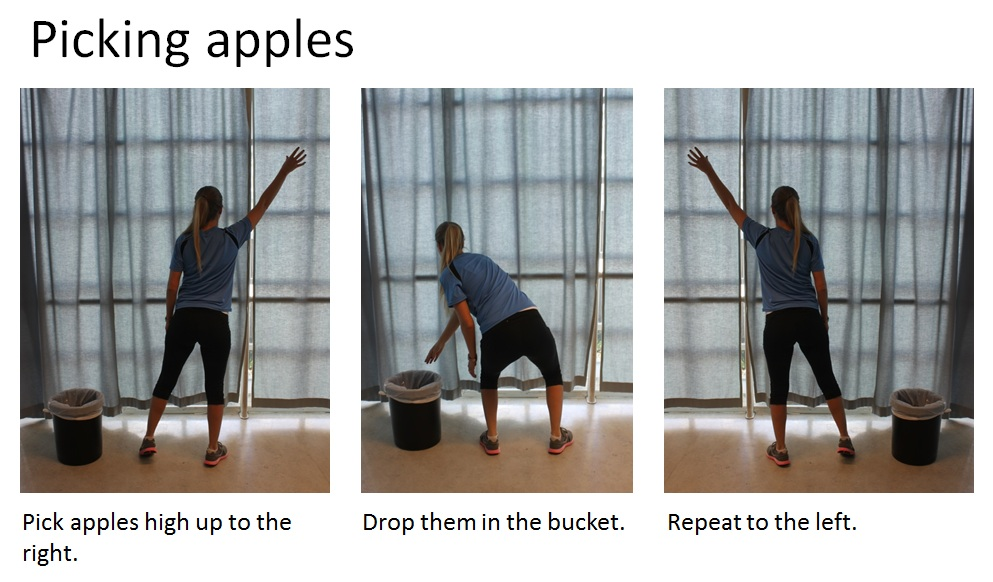
\includegraphics[scale=0.5]{PickingApplesAlone.jpg}
\caption[Exercise - picking apples]{The "Picking apples" exercise from \emph{Øvelsesbanken}.}
\label{pickingapples}
\end{figure}

\subsection{Instruction and Feedback}
In this exergame, the player will be given instruction about the technology, how to play, and how to perform various activities and exercises [req. 1.9-10]. When first starting the exergame, the player will be informed on how to interact with the Kinect sensor and the game. The player will be told that she has to use her body to engage game play, that she has to use her hand to navigate through the menu, and that she can make a choice by "pressing a button". 

In each of the five games there will be instructions informing about the goal of the game, the purpose of the various elements, and how the player should move to perform the activities in the game [req. 1.10]. There will also be provided information of the health benefit gained from performing the various activities [req. 1.11]. When the game starts, the overall purpose of the it is explained. This is for the player to know what is expected from her [req. 1.9-11]. Specific information about the various challenges will not be given all at once, as this will require a lot of memorisation. Therefore, these type of instructions will be given during game play, when there occur situations that makes it appropriate to provide the player with new information [req. 1.12]. This will be when the player meets new elements, obstacles or challenges. Every instruction comes with a button that the player has to push to continue playing. In this way the player is in the control of the game, and can decide for herself when she is finished reading the instruction [req. 1.13]. Figure \ref{fig:kineintro} shows an example of an instruction. The player will always be given the possibility to skip the instructions, so the experienced player do not have to watch the same instructions each time she plays [req. 1.14].

During game play, the player will be given appropriate feedback on her actions [req. 1.15-16]. This will be given when she has completed a particular task or activity, to not interrupt the player from performing ongoing tasks [req. 1.17]. Examples will be motivating comments, such as "Congratulations, you did a great job", when the player has accomplished balancing over a log, or "Lift your legs higher to walk faster". While playing, feedback should be given orally by a calm lady voice [req. 2.3]. Textual feedback during game play is avoided to not interfere with immersion and disturb the gaming experience [req. 1.17].  However, text can be chose instead of voice if if is preferred [req. 1.4]. 

\begin{figure} [H]
\centering

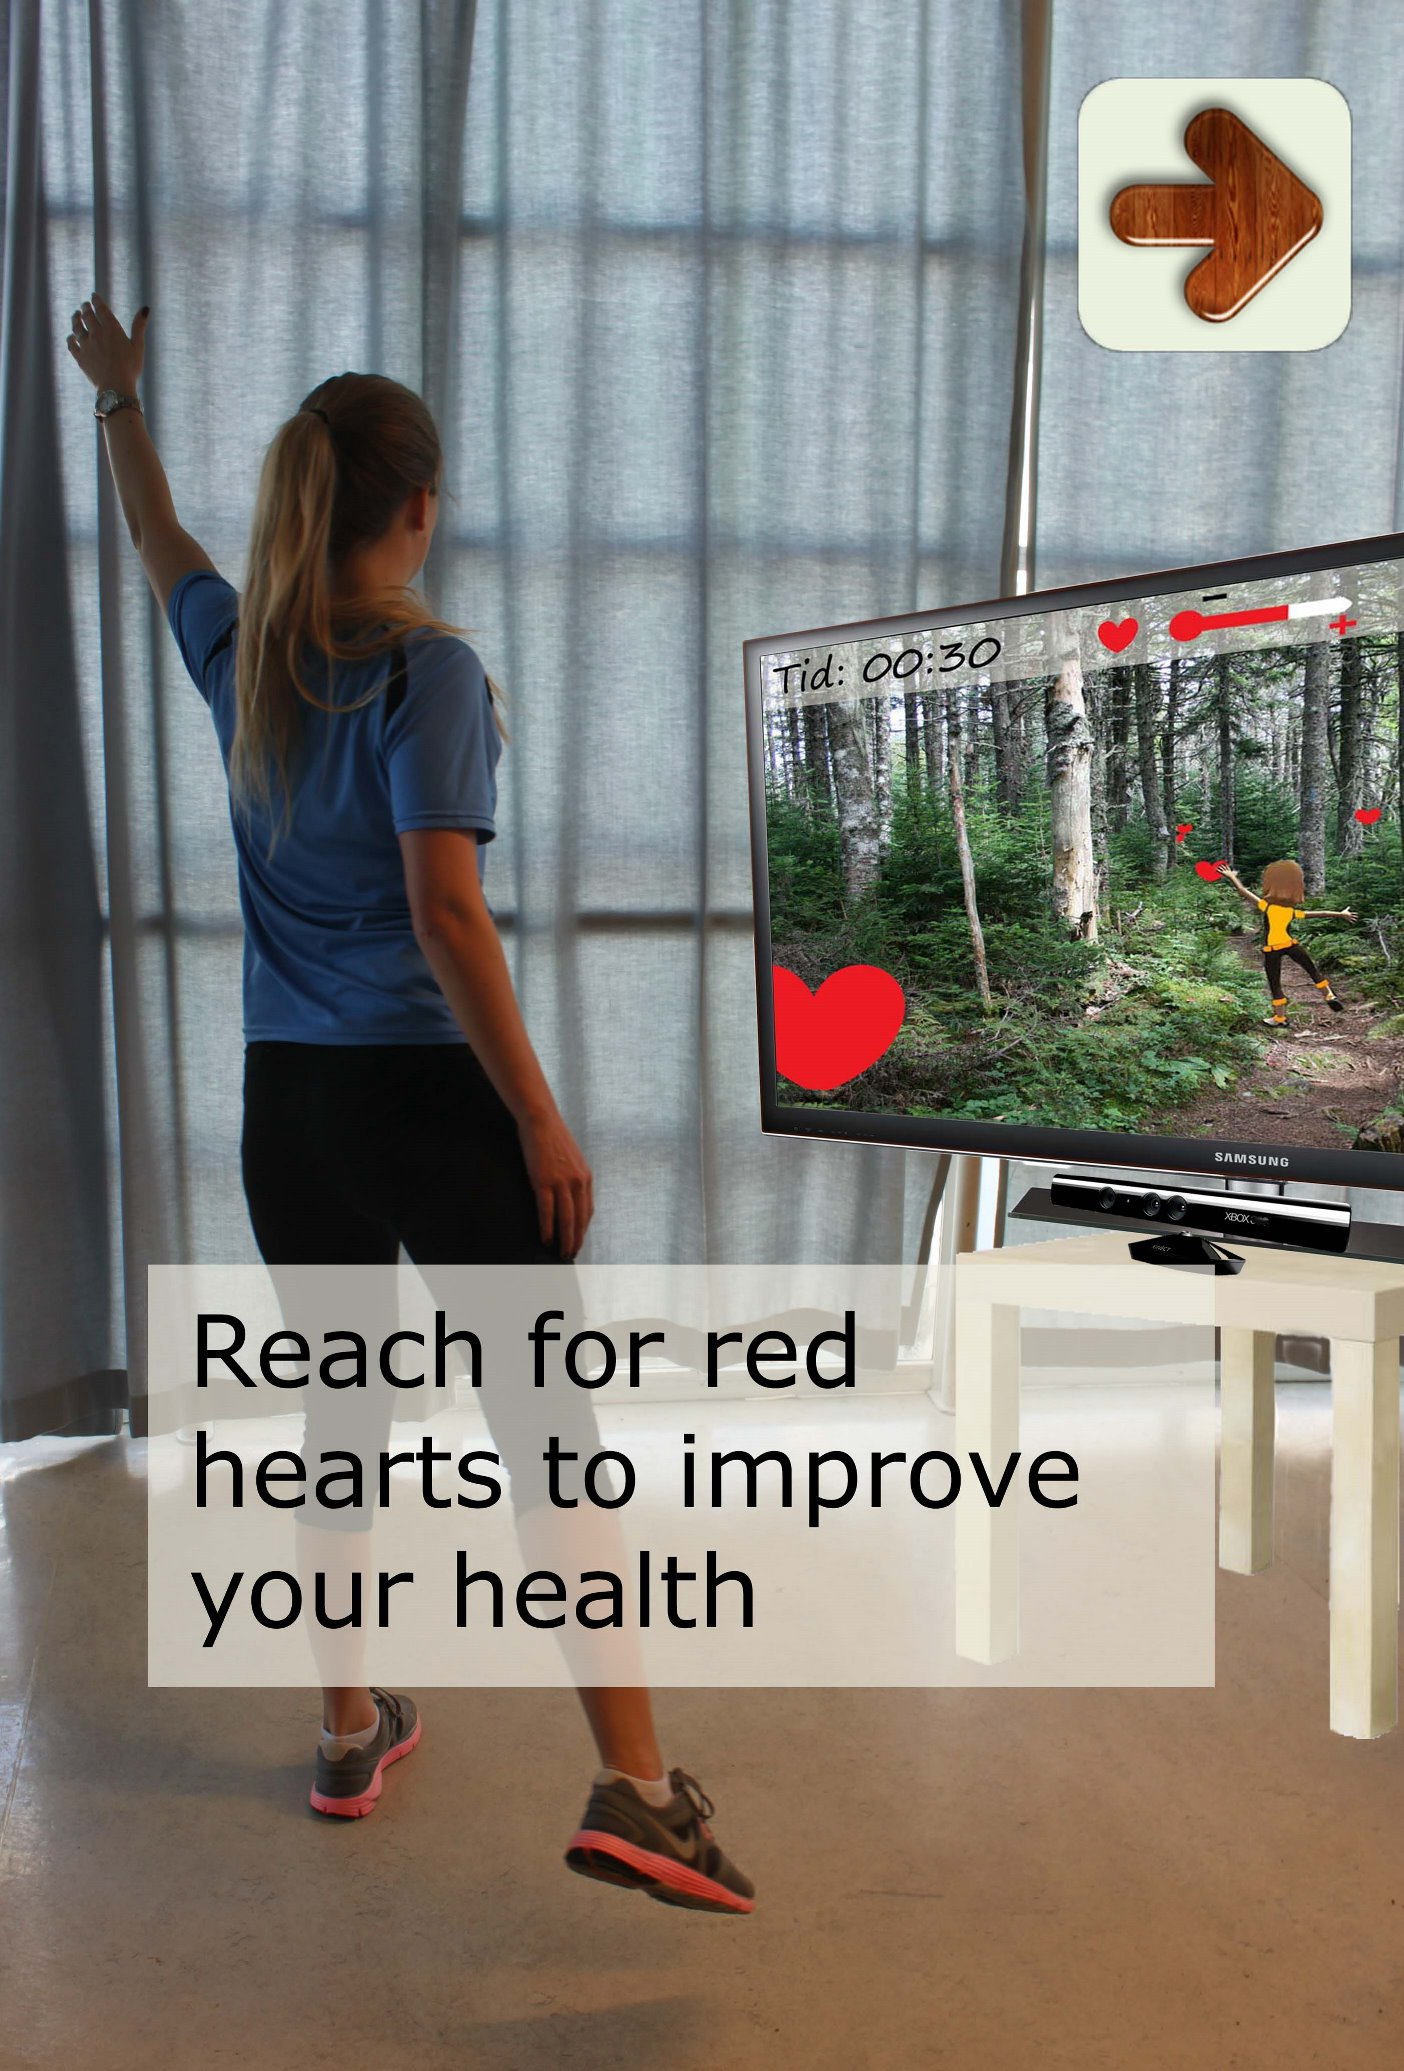
\includegraphics[scale=0.13]{introKineEng.jpg}
\caption[Instruction]{This figure shows an instruction in the exergame. There is a button up in the right corner that will be used to continue with the game when the player is done reading the information.}
\label{fig:kineintro}
\end{figure}

\subsection{Nature Trail}
The main activity in "Out in the Nature", is what we have called a "Nature Trail". This involves a walk in the forest with quizzes along the way. The goal for the game is to complete the nature trail as fast as possible, while answering questions, and avoiding obstacles on the way [req. 1.7]. Points will be given according to correct answers on the quiz, which will be shown up in the right corner together with a icon showing a sheet of paper. Because the Kinect sensor can track movement, points will also be given according to how well the player performs the required movements. These points will not be shown as numbers, as movements will be difficult to measure and "grade". Therefore, gain from correct and well-performed movements are shown in a "health-bar" on top of the screen [req. 1.20]. Showing this visually is also done to avoid too much detailed information, as suggested by Brox et al. \cite{exergamesforelderly}. A red heart is shown together with the bar to represent health. Points for correct answers on the quiz are separated from points achieved from movements, because the quiz has to do with cognitive skills, while the latter is about physical skills. The time used to complete the nature trail will affect the final result of the "health-bar", as this also reflects how well the player has moved during game play. See Figure \ref{fig:hearts} for an example of a scenario, which includes the described elements in the top-bar. "Nature Trail" supports the possibility to choose number of players, as multi-player mode enhance social interaction while playing [req. 1.8, 1.21].  

Progress in the game requires movement, like walking. When walking, the avatar portraying the player will walk into the forest. The bigger movements the player uses, e.g. the higher the player lifts her feet while walking, the higher pace, and "better health" she will achieve. Figure \ref{fig:hearts} shows an avatar in the forest, surrounded by hearts, where the avatar does a wide stretch trying to reach a heart. The hearts will be positioned in a way that will require the player to move to reach for them. Therefore, if the player gathers these hearts, her health will improve due to physical activity [req. 1.3]. Gain from gathering hearts will also be shown in the "health-bar".   

\begin{figure} [H]
\centering
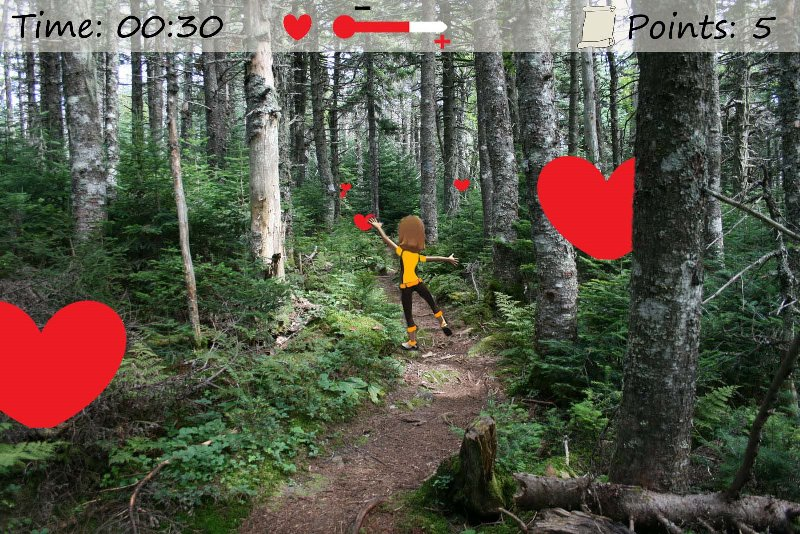
\includegraphics[scale=0.27]{game1engelsk.jpg}
\caption[Nature trail - stretching]{This figure presents a scene from the nature trail. We see an avatar in the forest, doing a wide stretch trying to reach a heart. This will result in improved health, shown in the "health-bar".}
\label{fig:hearts}
\end{figure}

The quiz in the nature trail will be shown as sheets of paper "hanging" on different spots in the forest. The player has to reach for them to get access to the questions, see Figure \ref{fig:quiz}. When picking a question, it will pop up and fill the screen. Four alternatives will be shown, and the player will have to use her hand to navigate to what she believes is the right answer. Questions will be chosen randomly, so the player do not get the same questions each time she plays. The difficulty will also increase in line with correct answers [req. 1.25]. The player does not have to answer the quiz to complete the nature trail [req. 1.8], but it will affect the total score at the end. 

\begin{figure} [H]
\centering
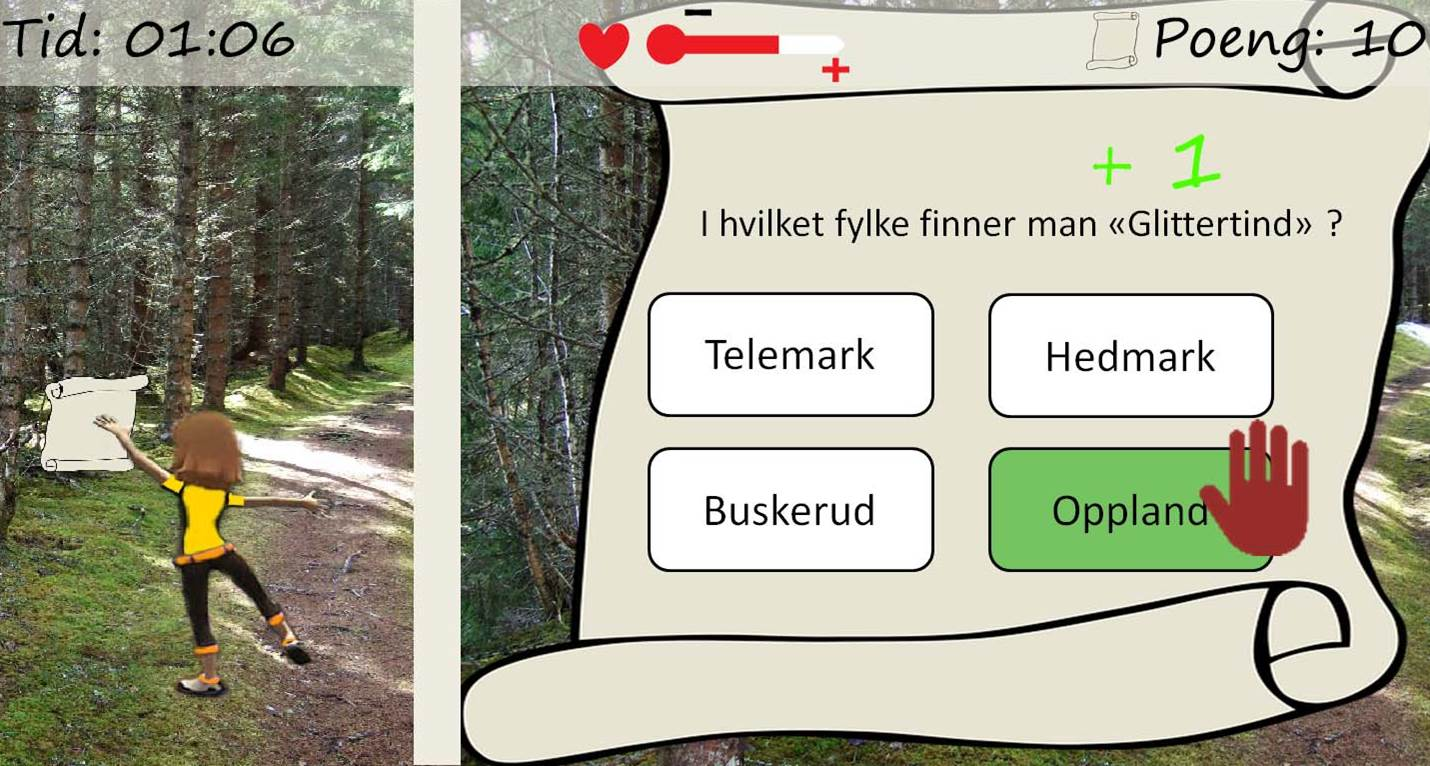
\includegraphics[scale=0.4]{quiz.jpg}
\caption[Nature trail - quiz]{The quiz in the nature trail will be shown as a piece of paper "hanging" on different spots in the forest. Questions will pop up and fill the screen. Here, the player is asked about where to find the Norwegian mountain "Glittertind".}
\label{fig:quiz}
\end{figure} 

Along the way in the nature trail there will be various, natural obstacles that will force the player to move her body in certain ways to be avoided. The game is suppose to exercise the whole body. Therefore, the different obstacles are chosen, so that the movements required to avoid them will include all muscle groups [req. 1.1, 1.3]. Examples of these obstacles are a river or creek that the player has to cross, or logs or rocks lying on the path that the player has to step over. To cross a river or creek the player has to balance on logs or step on rocks. This requires movements as toe-to-heel stepping, and step touch or skaters. When meeting a log, the player is required to take a big step, or a lunge, to get past it. Rocks in the path are avoided by performing sideways steps, or step-touch. There will also be obstacles in head hight, like branches, which require the player to go into deep squats to be avoided. The Kinect sensor will track the player's body, and increase or decrease the "health-bar" according to how well the player perform the required movements. If the player hits some of the obstacles, they will get a flash of red, indicating that the player failed to avoid them. As a result, the red color in the "health-bar" will decrease [req. 1.20].

Parts of the story are organised with the use of "branching", which is about having the possibility to choose between multiple paths [req. 1.8]. An example of this is choosing between walking the "regular" trail or rowing a boat over a lake. To cross the lake, and continue the nature trail, the player has to take a side step and step into the boat. To move forward, rowing movements are needed. There will be water lilies in the water which the player has to avoid. This is done by leaning the upper body over to the sides. This, and all the other described obstacles, are shown in Figure \ref{fig:hindring}. All the tasks the player has to do throughout the game will be described in the functional design, in Section \ref{sec:functionaldesign}. The reader is referred to Appendix B for detailed instructions on how to perform the various exercises.

\begin{figure} [H]
\centering
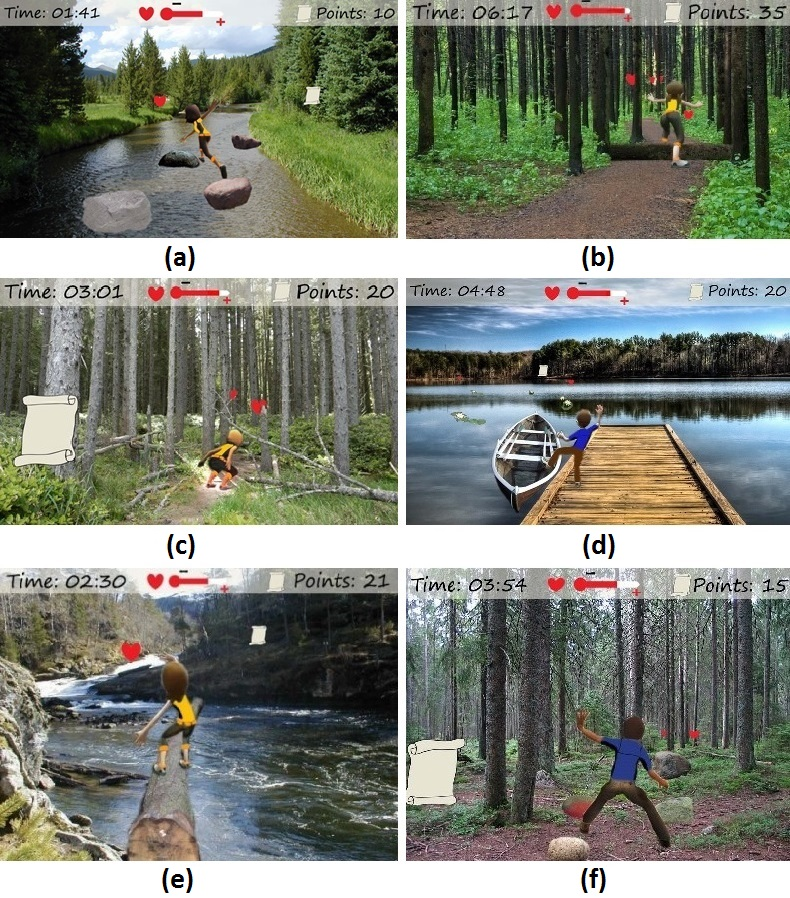
\includegraphics[scale=0.57]{hindringerEng.jpg}
\caption[Nature trail - obstacles]{This figure presents various obstacles to be found in the nature trail. a) jump from rock to rock to get over the river, b) walk over the log lying across the path, c) duck under the branch hanging over the path, d) get over the lake by rowing the boat, e) balance on the log to get over the river, f) walk pass the rocks lying on the path}
\label{fig:hindring}
\end{figure}

One of the requirements for this exergame is that the game has to show progress [req. 1.20]. In workshop 1, the informants told us that it was important to see that they learned something, and that they got better. They also expressed it as important to get the possibility to choose difficult levels themselves. We have solved this by having a step in the menu where the player can choose the preferred difficulty for the game, see Figure \ref{fig:omgivelseNivaa}. 

\begin{figure} [H]
\centering
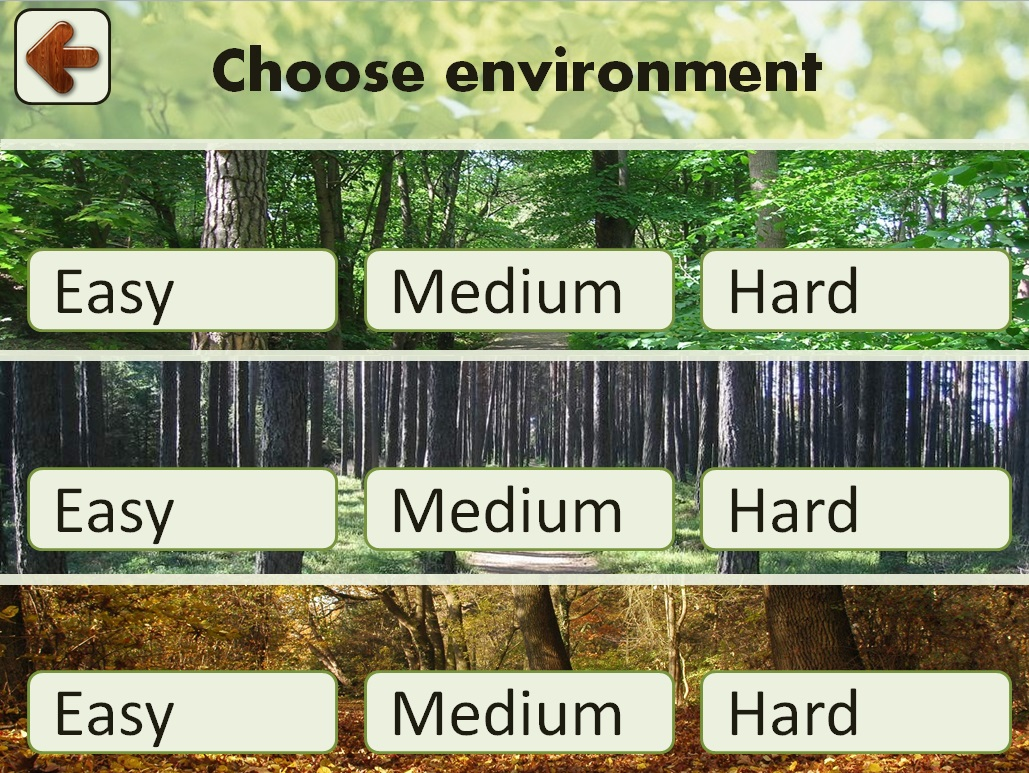
\includegraphics[scale=0.25]{chooseEnvironment.jpg}
\caption[Choice of environment and difficulty level]{When "Walk the Nature Trail" is chosen, players will get the possibility to choose environment and difficulty level. The environments to choose from are pine wood, deciduous wood summer, and deciduous wood fall; within each environment there are three difficulty levels.}
\label{fig:omgivelseNivaa}
\end{figure}

The "Nature Trail" game offers three different forest environments to walk in, a pine wood, and two deciduous woods, showing both summer and autumn. Each of the environments presents initially different difficulty levels, and within each environment, there are three difficulty levels: easy, medium, and hard [req. 1.8, 1.23]. First time playing, only the easy level will be available. The higher levels will be unlocked when the player has managed the easy level [req. 1.25]. A higher difficulty level will require more from the player, both mentally and physically. Obstacles will occur more frequently, which will require concentration, and the movements and exercises will be harder to perform, and therefore require control of the body. Within one environment, the obstacles from the easy level will follow to the next levels. This is done to include some familiar elements in the higher levels, in addition to new obstacles that will be added. To support variation between the environments, new and different obstacles will be used in each of the three environments.  

The required movement in the "Nature Trail" game are suppose to exercise the whole body. This involves endurance, balance, and exercise of several muscle groups. This game, with the quiz and movements combined, will be good for both cognitive skills and physical health.     

\subsection{The Four Single Games}
In addition to the nature trail, "Out in the Nature" consists of four shorter games with focus on completing one single familiar activity or challenge. The activities we have chosen for this exergame are wood chopping, paddling down a river, swimming in a lake, and picking apples [req. 1.4, 1.6]. Within each game the player has the possibility to choose number of players and difficulty level [req. 1.8, 1.21, 1.23]. In multi-player mode, players can choose if they want to cooperate or compete against each other. When competing, the players will have the possibility to select difficulty level individually. This is to allow for players with different experience to play together, like a grandmother and her grandchild [req. 1.24]. Figure \ref{fig:velgSpill} shows how these single games will be presented in a menu. Below, we will describe one of these four games in more detail.

\begin{figure} [H]
\centering
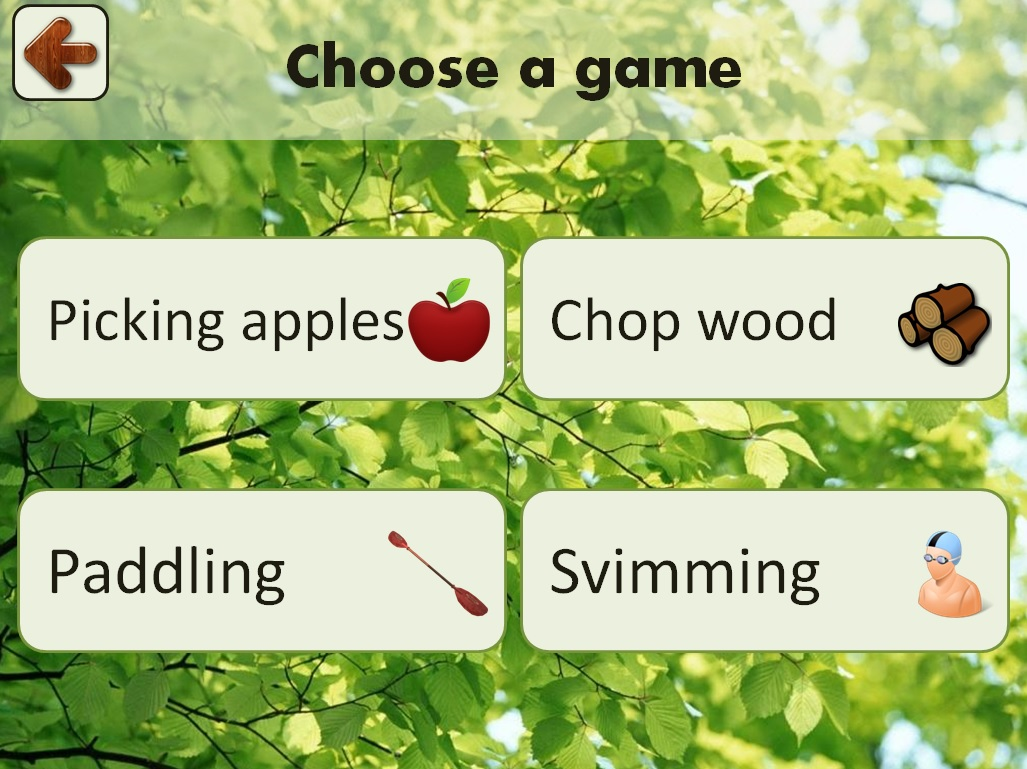
\includegraphics[scale=0.25]{chooseGame.jpg}
\caption[The four single games]{In addition to the "Nature Trail" game the players can choose between four single games: picking apples, chopping wood, paddling, and swimming.}
\label{fig:velgSpill}
\end{figure}

\subsubsection{Picking Apples}
"Picking Apples" is a game that requires squats and stretching exercises, which will strengthen balance and muscles in thighs and the gluteal area. The goal for this game is to pick as many red, ripe apples as possible in a given amount of time, and the apples should be put in baskets on the ground [req. 1.6]. This is shown in Figure \ref{fig:appleStretch} and \ref{fig:appleSquat}. The movements this game requires fit well with the one of the exercises chosen from \emph{Øvelsesbanken}(see Figure \ref{pickingapples}). When apples first appear on the tree they will be green, indicating that they are not ready to be picked. If ripe apples are left hanging on the tree for too long, they will rot and fall to the ground. Rotten apples will have a brown color. 

\begin{figure} [H]
\centering
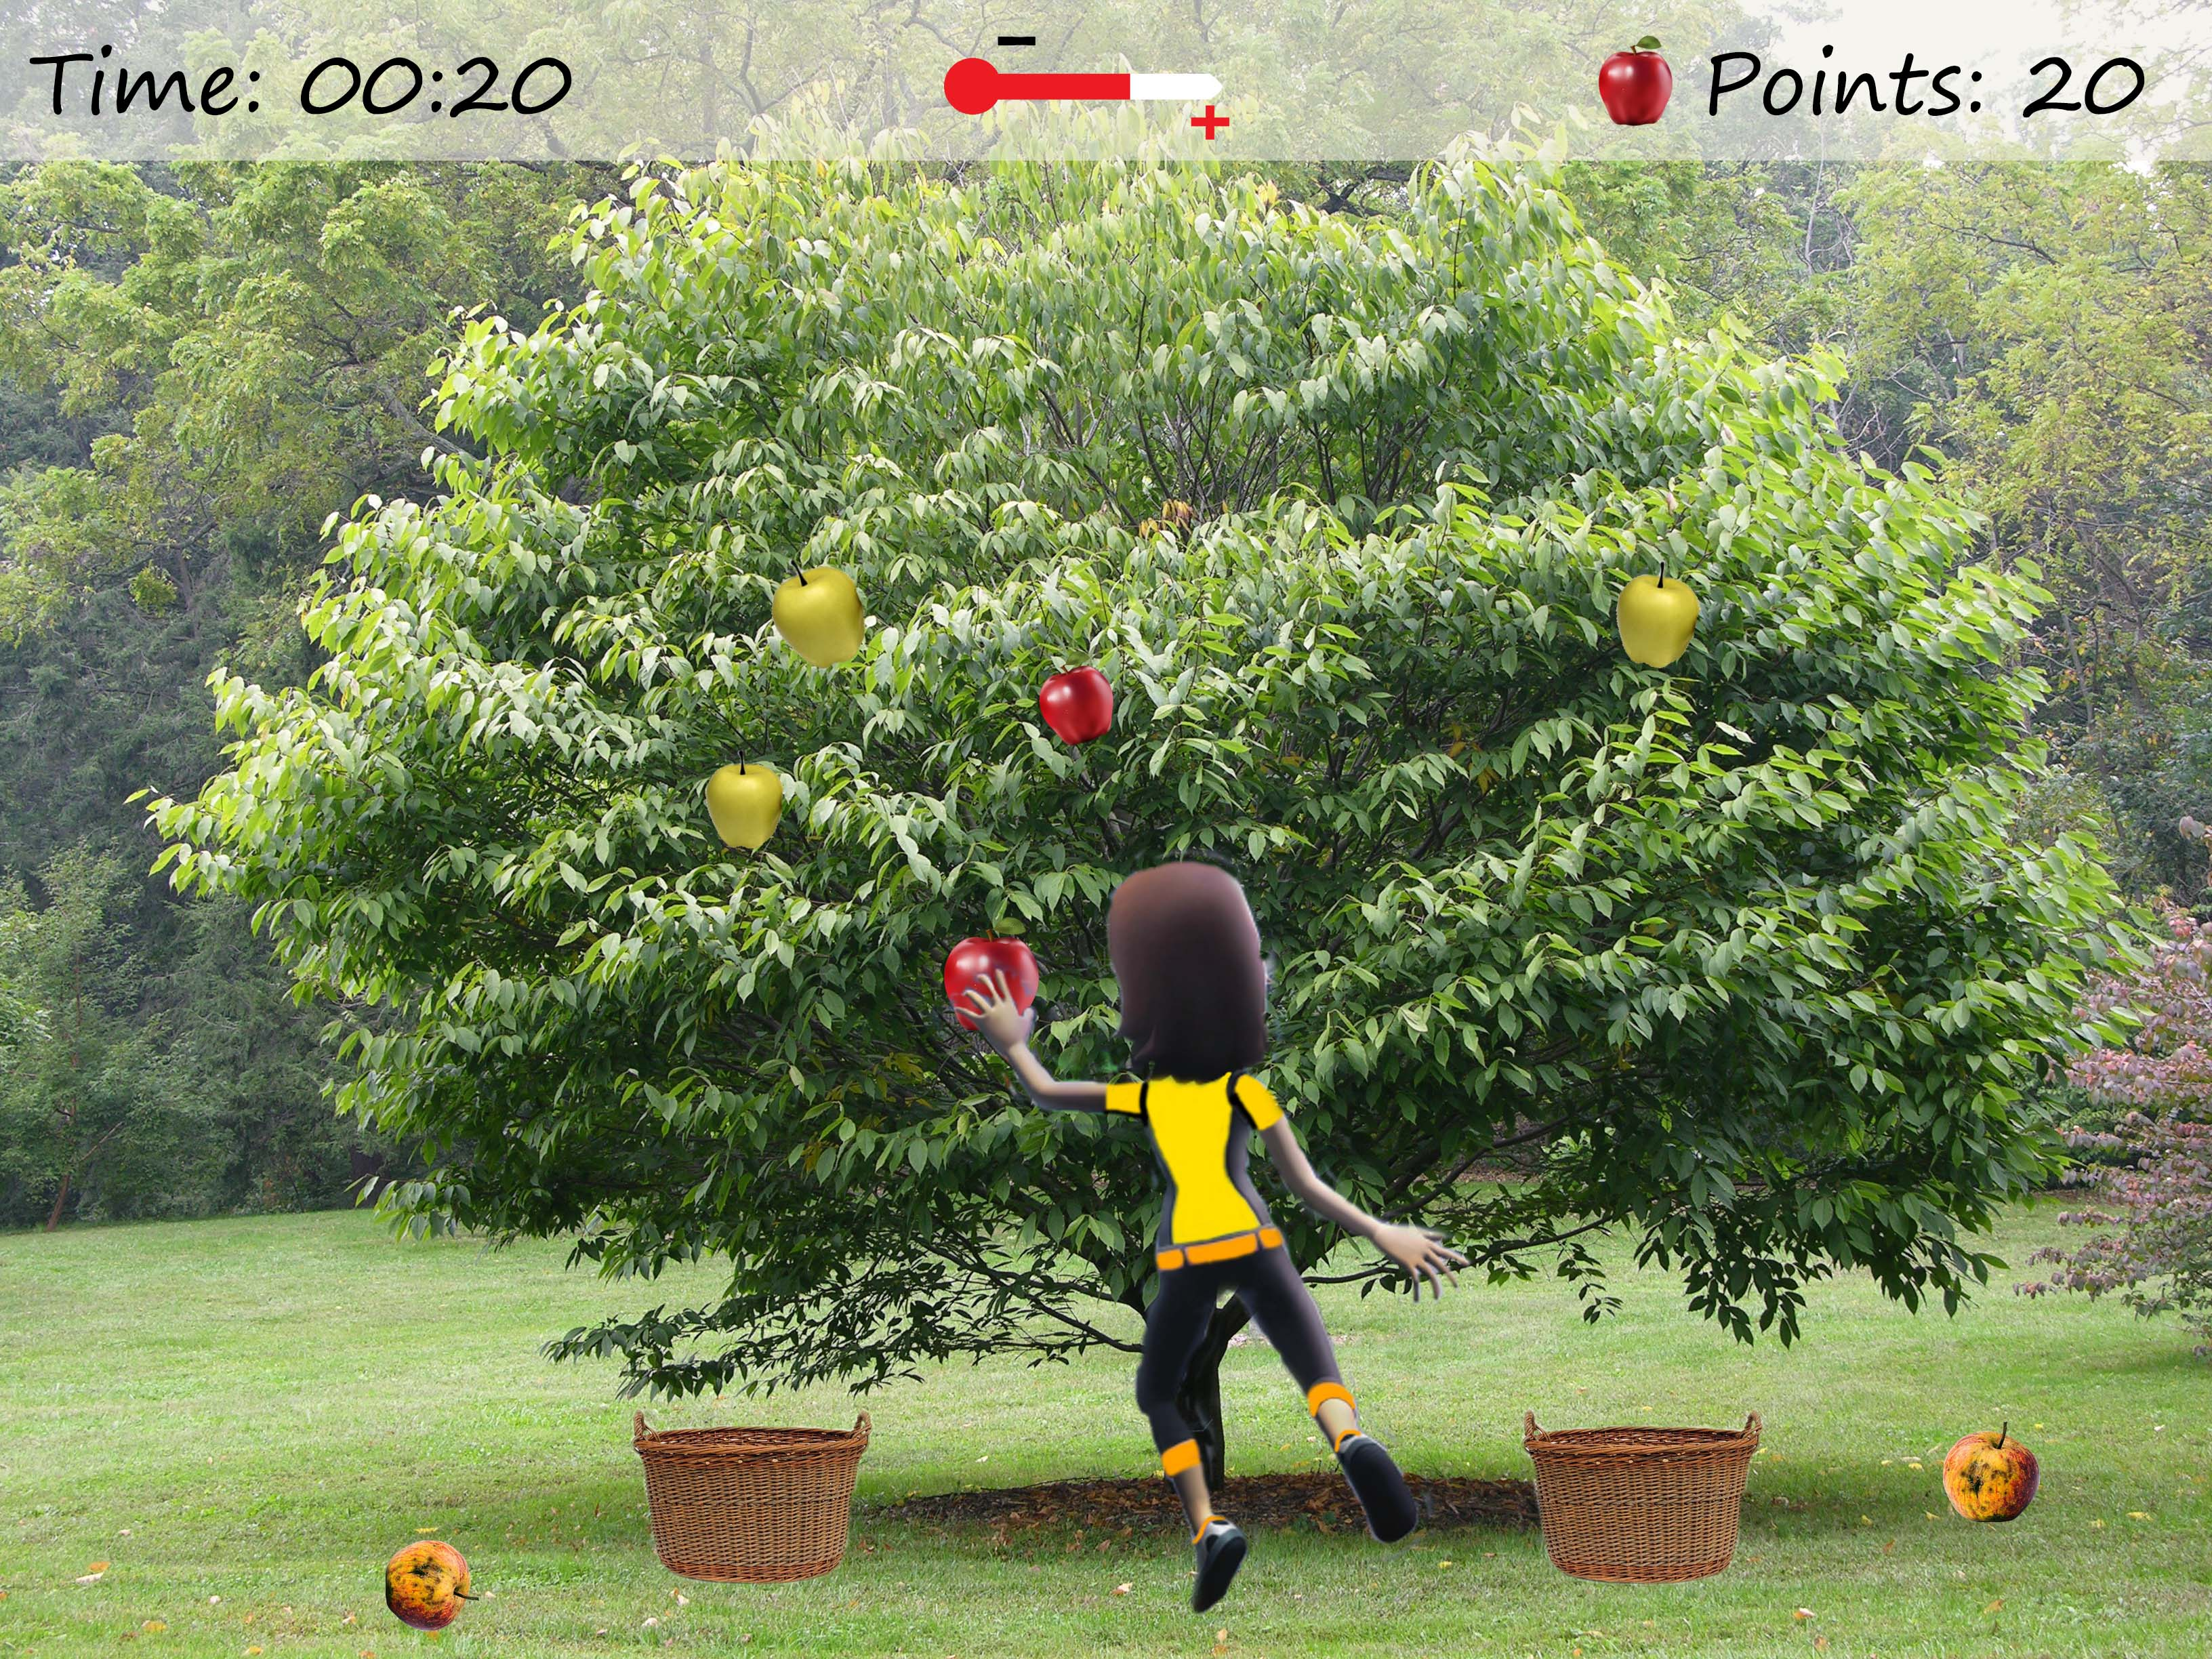
\includegraphics[scale=0.07]{gameappletreeEng.jpg}
\caption[Picking apples - stretching]{The player stretches up to pick a red, ripe apple. We observe that there are, in addition to red apples, three green apples on the tree, and two rotten on the ground.}
\label{fig:appleStretch}
\end{figure}

\begin{figure} [H]
\centering
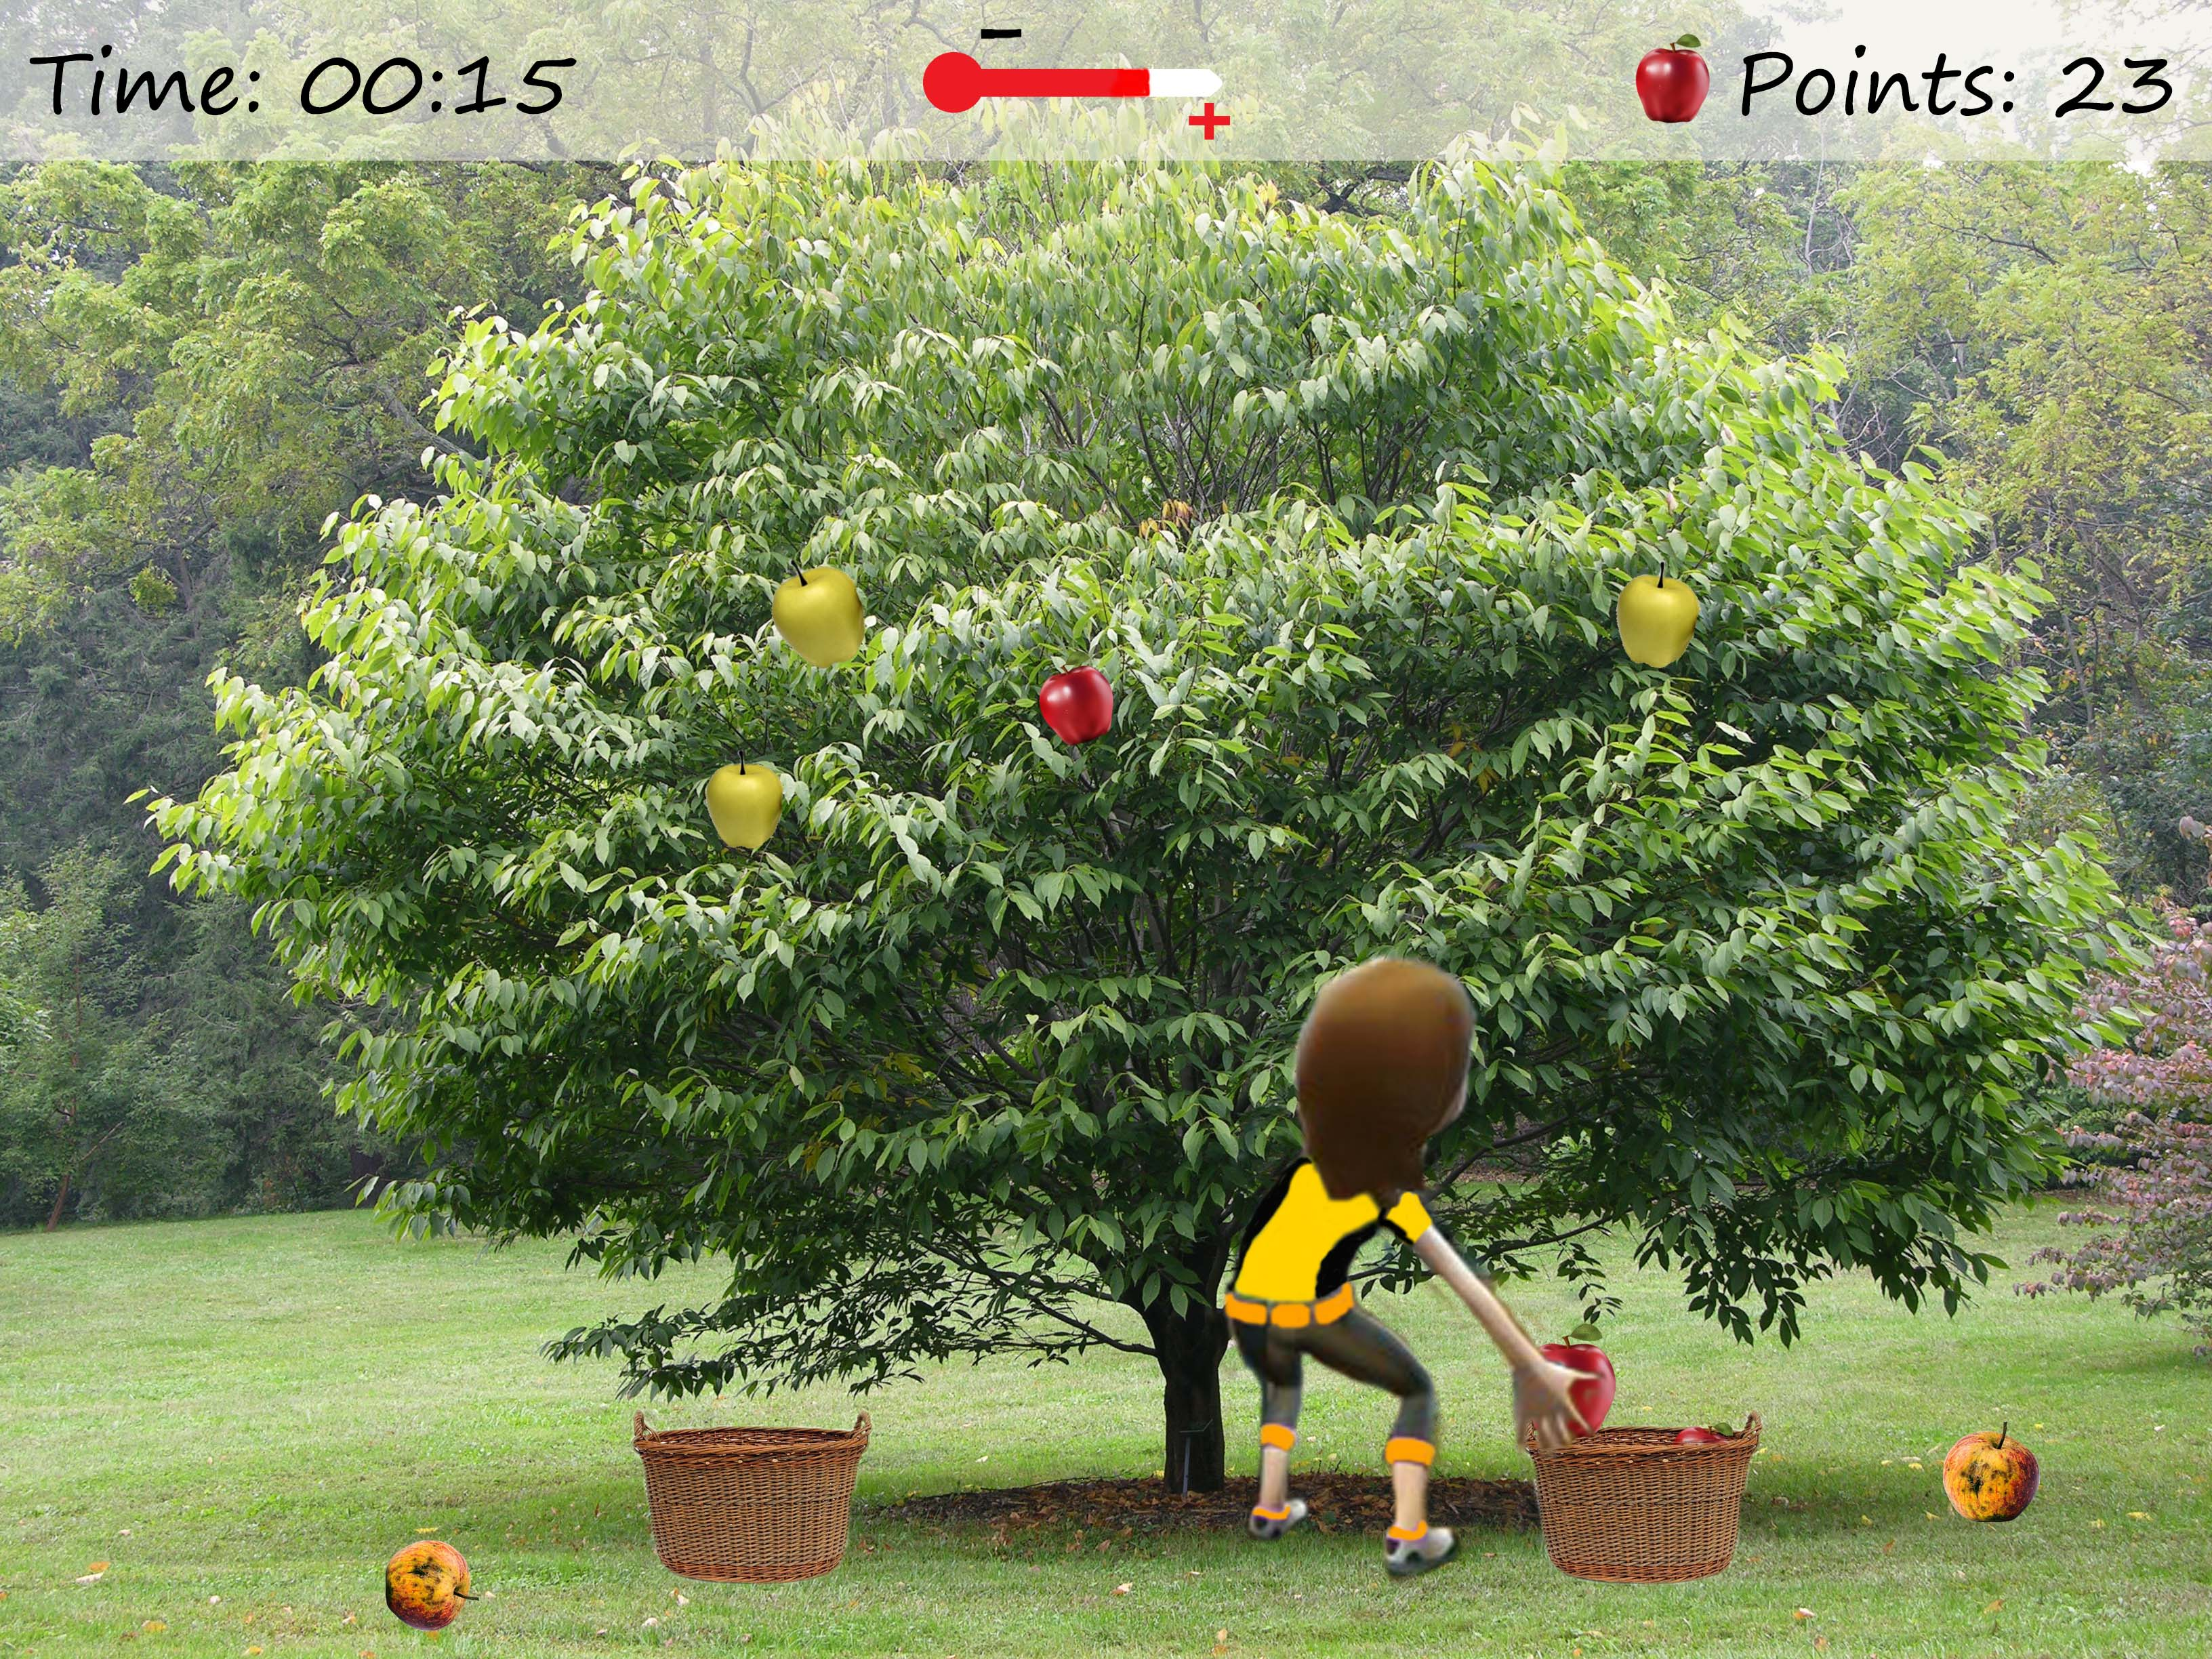
\includegraphics[scale=0.07]{squatppletreeEng.jpg}
\caption[Picking apples - squats]{The player has picked a red apple and is about to put it in the basket. The player uses deep squats to perform this action.}
\label{fig:appleSquat}
\end{figure}

Points will be given according to how many apples the player has picked, see Figure \ref{fig:appleOver}. 3 points will be given for each ripe apple that is picked and put in a basket. The player will loose points if green apples are picked, or if apples have been given the time to rot. Picking a green apple will result in -1 point, and if the apple gets rotten this will result in -2 points. If the player does not perform squats when putting apples in a basket, there is a great possibility that the apple will miss the basket and fall to the ground. This will give the same loss of points as a rotten apple, i.e. -2 points.       

\begin{figure} [H]
\centering
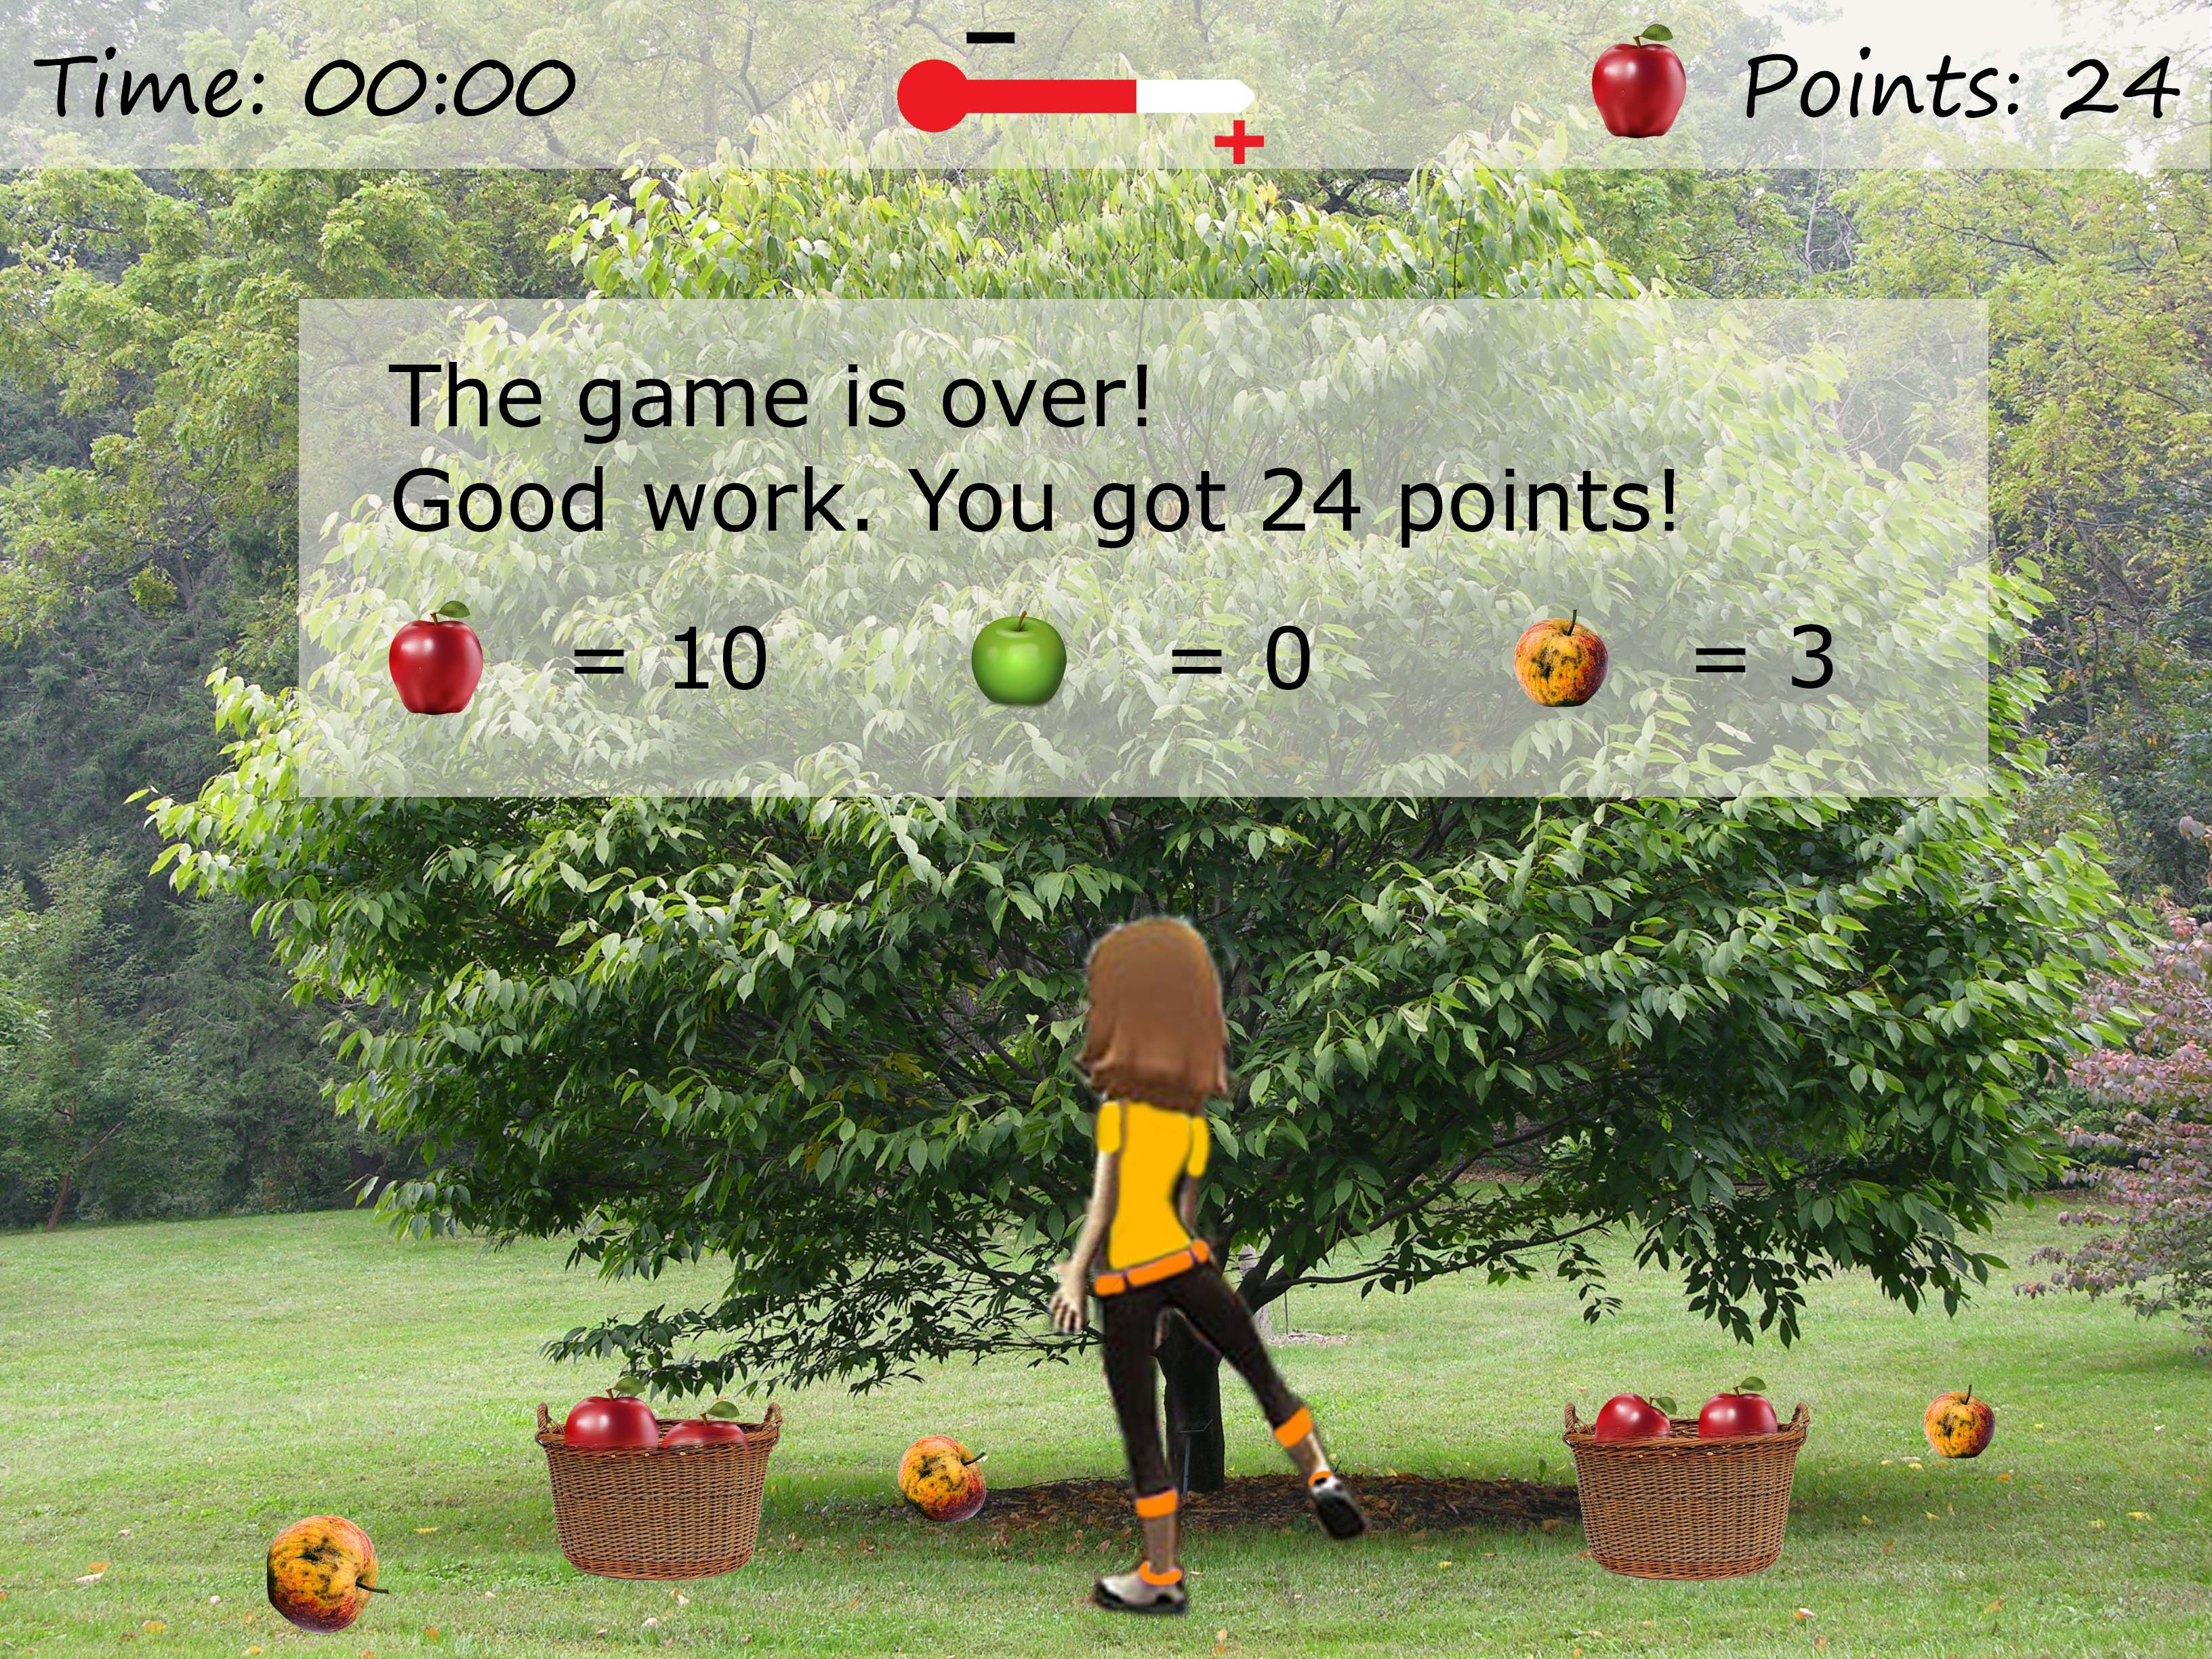
\includegraphics[scale=0.07]{appletreeendEng.jpg}
\caption[Picking apples - points]{This figure presents a final scene in the "Picking Apples" game. A text, together with the number of apples picked, is shown.}
\label{fig:appleOver}
\end{figure}

Apples will appear on the tree and grow in a certain tempo according to the chosen difficult level. Higher difficulty will result in more apples on the tree at the same time, and a faster ripening rate. An extra challenge in the higher difficulty level is additional requirements to the two baskets, in which the newly picked apple should be put. This is to train cognitive skills and to include more variation in movements and exercises [req. 1.24]. As mentioned, this game allows for multi-player mode where the players can collaborate on picking apples, or compete on who can pick the most apples [req. 1.22], see Figure \ref{fig:appleMultiplayer}. 

\begin{figure} [H]
\centering
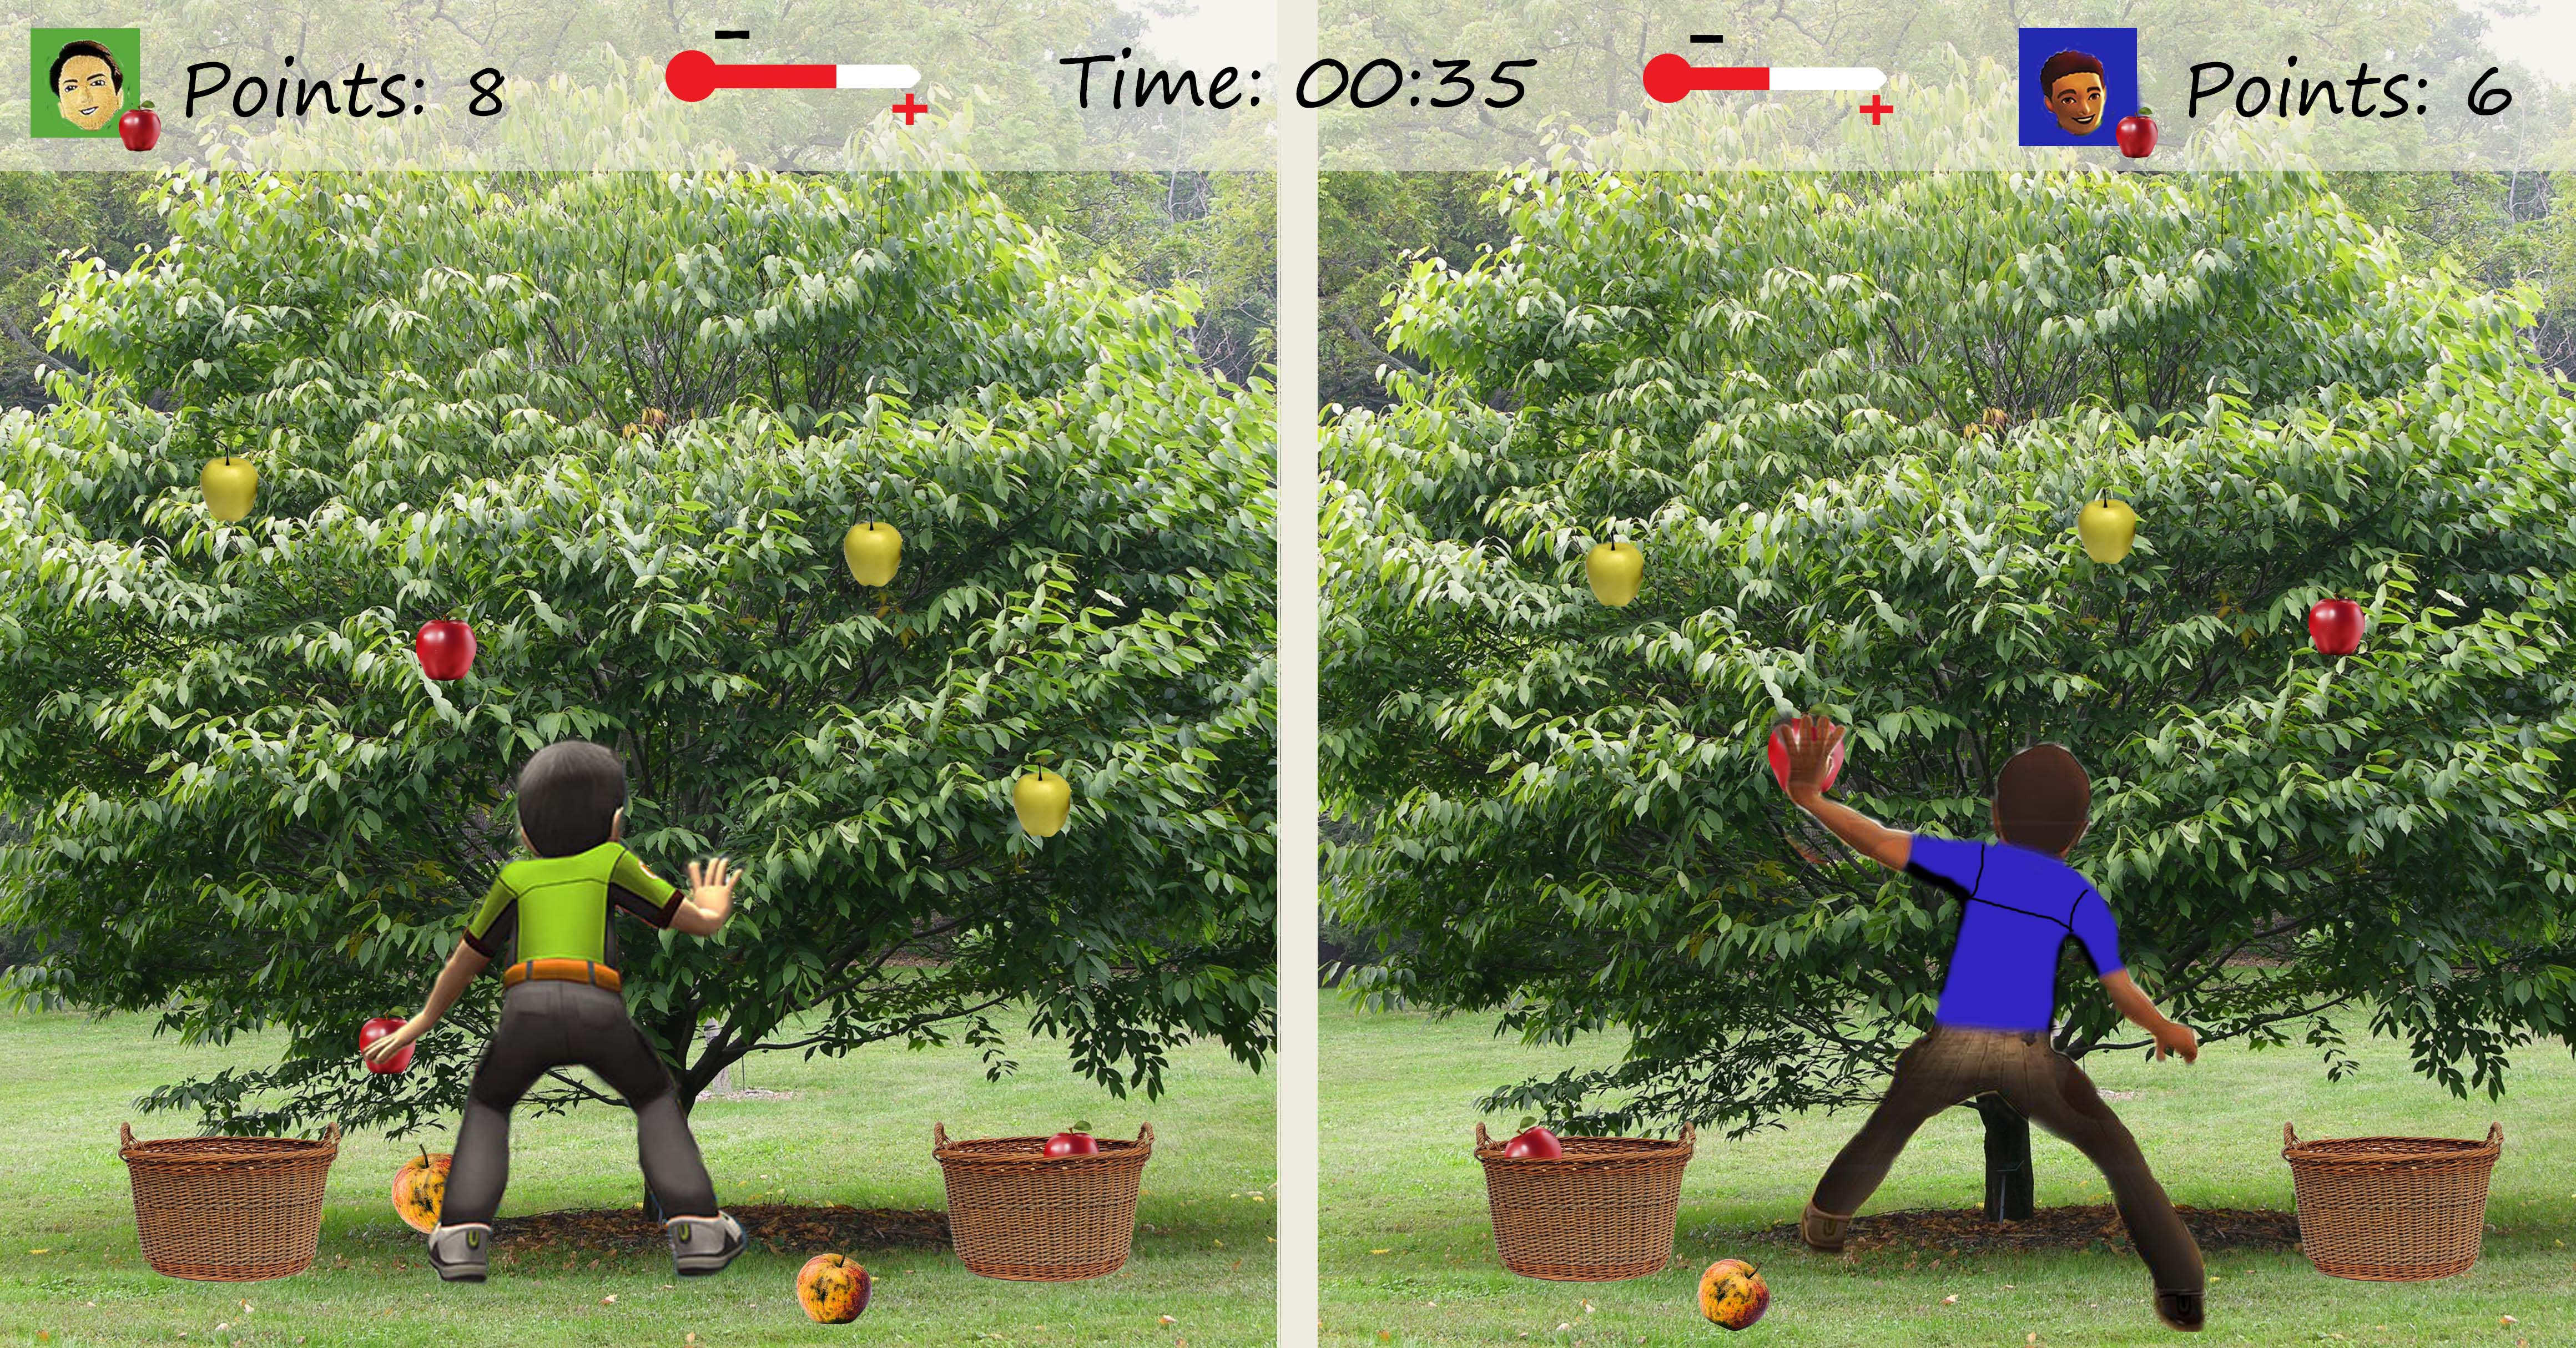
\includegraphics[scale=0.07]{gameapple2playerEngelsk.jpg}
\caption[Picking apples - multi-player]{In this figure we observe two players playing together in competitive mode.}
\label{fig:appleMultiplayer}
\end{figure}

\section{Functional Design}
\label{sec:functionaldesign}

The functional design for this game will be described according to system requirements presented in Section \ref{sec:req}, and to video game theory discussed in Chapter \ref{chap:vg}. The functional design will provide a more concrete representation of the exergame, than what have been presented earlier in this chapter. Here, all the elements the game should contain will be presented shortly. Functional design will vary according to the chosen difficulty level, however, in this thesis we will only focus on presenting functional design for one difficulty level for each game.

We will describe functional design for what we have presented in this exergame concept, i.e. the "Nature Trail" and "Picking Apples". This will, as mentioned, be described according to video game theory, and more specifically to the game's story and aesthetics.  

\subsection{Nature Trail}

\subsubsection{The Fictional World} 

\begin{table} [H]
\centering
\begin{tabular}{|p{3,2cm}|p{7,8cm}|}
\hline
\emph{Location/setting} & In the pine forest  \\ \hline
\emph{Structural objects} & Trees, the trail, heaven, rocks, log, anthill, lake, puddle, creek, river.  \\ \hline
\emph{Interactive objects} & The player character, row boat with oars, rocks lying in the middle of the trail, rocks in the river, logs over a creek, red hearts in the field, branches, question sheets, log lying across the trail. \\ \hline
\emph{Scripting objects} & Quiz points: Shown as an icon similar to a sheet of paper, with the text "points" after it. Increments with 5 points as the player answer the right question.\\ \hline
	     & "Health-bar": Increases as player performs right movements. Decreases as player does not manage the right movements. Increases when player gathers hearts. Increases based on time spend in game world compared to previous sessions. 
	      \\ \hline
	       & Time: Increases as a normal clock \\ \hline
\emph{Characters} & An avatar (from how Kinect defines a character) seen in third-person perspective, described by its name. \\ \hline
    \end{tabular}
    \caption[Various objects in the "Nature Trail"]{Different types of objects}
    \label{tab:objects1}
\end{table}  

\subsubsection{Mechanics} 

The game is a progression game, where a story should be completed. Each level will be completed by solving puzzles. The player has to finish different quests within a level to proceed to the next level, and the levels build on each other. It is common to have a climax at the end of each chapter in these type of games. However, this is not included here, as this will interfere with the natural environment and the gaming experience for this type of users. In Table \ref{tab:quests1} we will present different quests in the "Nature Trail" game. 
  
\begin{table}
\begin{tabular}{|>{\raggedright}p{7,5cm}|p{3,5cm}|}
\hline
\textbf{Quest} & \textbf{Exercise required}  \\ \hline
Walk the trail to get forward in the forest & Lift legs high, walking  \\ \hline
Gather hearts and "get better health" &  Stretching \\ \hline
Walk past rocks lying in the middle of the trail & Side steps or step touch  \\ \hline
Duck under branches hanging over the trail & Squats
\\ \hline
Balance over the log to get to the other side of the creek & Toe-to-heel stepping with arms out \\ \hline
Walk over the log lying across the trail & Lunges \\ \hline
Jump from rock to rock to get over the creek & Step touch or skaters \\ \hline
Row boat over to the other side of the lake & Rowing \\ \hline
Row past the water lilies & Lean upper body from side to side \\ \hline
Find and get question sheets  & Stretching \\ \hline
Answer one of the four alternatives & Use knowledge and cognitive skills \\ \hline
Solve puzzle & Use knowledge and cognitive skills \\ \hline
\end{tabular}
\caption[Quests in the "Nature trail" game]{Quests}
\label{tab:quests1}
\end{table}
 
\emph{Branching} \\ \\ 
"Branching": Trail splits, and there are two possibilities: 1. Walk one trail with rock obstacles but a lots of hearts to gather. This will require some more time, but the player can gain more points by gathering hearts. 2. Walk the other trail which is without obstacles but no hearts to gather. 

"Branching": Trail splits, and there are two possibilities: 1. Keep walking the trail. 2. Row a boat over to the other side. Rowing requires legs wide apart and arms stretched out in front of the player and dragged back to their body, as actual rowing movements. 

\subsubsection{Rules} 
 
\begin{table} [H]
\centering
\begin{tabular}{|p{2,8cm}|p{8,2cm}|}
\hline
\emph{Interplay rules} & \textbf{1. The player character:} Will move to the movements received as player input. \\ \cline{2-2}
&  \textbf{2. Red hearts:} When touched by the avatar it disappears. \\ \cline{2-2}
& \textbf{3. Rocks lying in the middle of the trail:} If hit, the  rocks will flash red.  \\ \cline{2-2}
&  \textbf{4. Branch:} If hit, it will flash red \\ \cline{2-2}
& \textbf{5. Log over creek:} If the avatar falls off, the log will flash red. \\ \cline{2-2}
& \textbf{6. Log across the trail:} If hit, the log will flash red.  \\ \cline{2-2}
& \textbf{7. Rocks in the river:} If the avatar falls of a rock, the rock will flash red.  \\ \cline{2-2}
& \textbf{8. Rowboat with oars:} will move forward as the player  uses her arms with the oars. \\ \cline{2-2}
& \textbf{9. Water lilies:} If hit, the water lily will flash red \\ \cline{2-2}
&  \textbf{10. Question sheets:} When touched by the avatar  it  disappears from the game environment and fills the screen with  a  question or puzzle. \\ \hline
\emph{Evaluation rules} & \textbf{if 1}: Player gets forward in the game, and the health-bar fills with red color. \\ \cline{2-2}
& \textbf{if 2:} The health-bar fills with red color.  \\ \cline{2-2}
& \textbf{if 3:} Player gets slowed down, and red color in the health-bar reduces.   \\ \cline{2-2}
& \textbf{if 4:} Player gets slowed down, and red color in the health-bar reduces.  \\ \cline{2-2}
& \textbf{if 5:} Player gets slowed down, and red color in the health-bar reduces   \\ \cline{2-2}
& \textbf{if 6:} Player gets slowed down, and red color in the health-bar reduces   \\ \hline
\end{tabular}
\caption[Rules in the "Nature Trail" game]{Rules}
\label{tab:rules1}
\end{table} 

\begin{table} [H]
\centering
\begin{tabular}{|p{2,8cm}|p{8,2cm}|}
\hline
\emph{Evaluation rules} & \textbf{if 7:} Player gets slowed down, and red color in the health-bar reduces   \\ \cline{2-2}
& \textbf{if 8:} Player gets forward in the game, and the health-bar fills with red color.   \\ \cline{2-2}
& \textbf{if 9:} Player gets slowed down, and red color in the health-bar reduces   \\ \cline{2-2}
& \textbf{if 10:} If player answers right she gets +5 points. If player answers wrong she gets 0 points.  \\ \hline
\end{tabular}
\caption[Rules in the "Nature Trail" game]{Rules continues}
\label{tab:rules11}
\end{table}  

\subsubsection{Geography and Representation}

\begin{table} [H]
\centering
\begin{tabular}{|p{2,7cm}|p{8,3cm}|}
\hline
\emph{Music} & Calm, classical music that changes to the speed of the game and to certain happenings. \\ \hline
\emph{Vocalization} & The avatar will not have its own voice. \\ \hline
\emph{Sound effects} &  When hearts are gathered there is a cheerful "pling" sound.  \\ \cline{2-2}
&  When taking the question sheet there is a "swosj" sound.\\ \cline{2-2}
& When the avatar is walking there is the sound of steps on the ground. Different sounds for \\ & different surface, like walking on the rocks, soil or logs.\\ \cline{2-2}
& The sound of shoved water when rowing. \\ \hline
\emph{Ambient effects} & Birdsong. \\ \cline{2-2}
& Wind. \\ \cline{2-2}
& Water flowing in the river. \\ \cline{2-2}
& Waves from the lake.\\ \hline
\emph{Feedback} & Calm lady voice. \\ \hline
\end{tabular}
\caption[Different types of sound]{Different types of sound}
\label{tab:sound1}
\end{table}  

\begin{table} [H]
\centering
\begin{tabular}{|p{2,5cm}|p{8,5cm}|}
\hline
\emph {Perspective} & Third-person. \\ \hline
\emph{Dimension} &  3-dimensional and isometric. \\ \hline
\emph{Exploration} & Desired pace. \\ \hline
\emph{Saving} & The game will be able to save current state, progress and results. \\ \hline
\emph{Graphical representation} & The environment will be presented as close to photorealism as possible.  However, there will be some unrealistic elements present in the game environment.  \\ \hline
\end{tabular}
\caption[Graphical game characteristics]{Graphical game characteristics}
\label{tab:graphical1}
\end{table}  

\subsubsection{Number of Players}
The game supports two simultaneous players. The players can either compete or cooperate.

\subsection{Picking Apples}

\subsubsection{The Fictional World} 

\begin{table} [H]
\centering
\begin{tabular}{|p{3,2cm}|p{7,8cm}|}
\hline
\emph{Location/setting} & The player stands on a lawn with an apple tree in front of her. \\ \hline
\emph{Structural objects} & Tree, grass, heaven.  \\ \hline
\emph{Interactive objects} & The player character, apples on the tree, two baskets, one on each side of the player. \\ \hline
\emph{Scripting objects} &  Points: Shown as an apple icon with the text "points" after it. Increments with 3 points as ripe apples are picked and decrements with -1 point if an unripe apple is picked, and -2 points if an apple gets rotten \\ \cline{2-2}
& "Health-bar": Increases as player performs right  movements. Decreases as player does not manage the right  movements.  \\ \cline{2-2}
& Time: Decrease from 2 minutes \\ \hline
\emph{Characters} & An avatar (from how Kinect defines a character) seen in third-person perspective, described by its name. \\ \hline
\end{tabular}
\caption[Various objects in the "Picking Apples" game]{Different type of objects}
\label{tab:objects2}
\end{table}  
 
\subsubsection{Mechanics} 
This is a progression game where different levels of the game gets finished by solving the apple-picking task. The player has to finish different levels to proceed to the next level. The levels build on each other and the difficulty level gets higher as the player proceeds through the game.

\emph{Quests:} 

\begin{table}
\begin{tabular}{|>{\raggedright}p{7,5cm}|p{3,5cm}|}
\hline
\textbf{Quests} & \textbf{Exercise required}  \\ \hline
Pick apples when they get red and ripe & Stretching  \\ \hline
Put ripe apples in baskets &  Squats with downward arm movement \\ \hline
\end{tabular}
\caption[Quests in the "Apple Picking" game]{Quests}
\label{tab:quests2}
\end{table}

\subsubsection{Rules} 

\begin{table} [H]
\centering
\begin{tabular}{|p{2,8cm}|p{8,2cm}|}
\hline
\emph{Interplay rules} & \textbf{1. The player character:} Will move to the movements received as player input. \\ \cline{2-2}
 &  \textbf{2. Apples on the tree:} Will appear on the tree with a yellow-green color showing they are not yet ripe. After a while they will start to get red, and if the apples does not get picked while they are red, they will become brown and fall to the grown. \\ \cline{2-2}
& \textbf{3. Baskets:} The baskets will get filled with apples. \\ \hline
\emph{Evaluation rules} & \textbf{if 1:} Player proceeds through the game, and the health-bar fills with red color.\\ \cline{2-2}
 & \textbf{if 2:} If player picks a ripe apple she gets +3 points. If apple becomes rotten the player gets -2 points. If the player picks an unripe apple she gets -1 point. \\ \cline{2-2}
& \textbf{if 3:} If the player puts ripe apple in the basket she keeps the 3 points. If the player miss the basket, she lose 2 points.  \\ \hline
\end{tabular}
\caption[Rules for the "Apple Picking" game]{Rules}
\label{tab:rules2}
\end{table}  

\subsubsection{Geography and Representation}

\begin{table} [H]
\centering
\begin{tabular}{|p{2,7cm}|p{8,3cm}|}
\hline
{Music} & Calm, classical music that changes to the speed of the game and to certain happenings. \\ \hline
\emph{Vocalization} & The character will not have its own voice. \\ \hline
\emph{Sound effects} & Apples making a "pling" sound when getting picked.  \\ \cline{2-2}
&  Apples hitting the ground when falling from the tree. \\ \hline
\emph{Ambient effects} & Birdsong. \\ \cline{2-2}
& Wind. \\ \hline
\emph{Feedback} & Calm lady voice. \\ \hline
\end{tabular}
\caption[Different types of sounds in the "Apple Picking" game]{Different types of sound}
\label{tab:sound2}
\end{table}  

\begin{table} [H]
\centering
\begin{tabular}{|p{2,5cm}|p{8,5cm}|}
\hline
\emph {Perspective} & Third-person \\ \hline
\emph{Dimension} &  3-dimensional and isometric \\ \hline
\emph{Exploration} &  A mix between forced and desired pace. The pace is forced because the apples appear at random times. At the same time the pace is desired because the player can choose when she wants to stretch to gather the apple. However, this will also mean that the player chooses to lose an apple. Ripening pace will depend on current difficulty level.\\ \hline
\emph{Saving} & The game will be able to save current state, progress and results. \\ \hline
\emph{Graphical representation} & The environment will be presented as close to photorealism as possible.  \\ \hline
\end{tabular}
\caption[Graphical game characteristics in the "Apple Picking" game]{Graphical game characteristics}
\label{tab:graphical2}
\end{table}  

\subsubsection{Number of Players} 
The game supports two simultaneous players. The players can either compete or cooperate. 


\section{The Menu}
\label{sec:menu}

One of the main problems we observed during workshop 1 was related to handling the menus in the different games played. The general perception from workshop 1 was that the menus were complex, difficult to follow, demanding to navigate through, and too sensitive. This was also our own experience from playing. Therefore, we have made a prototype of a menu, which will be presented in this section.

The design of our menu proposal is based upon the interface requirements. Simple design, distinct elements, and easy to read information are emphasised to make it user-friendly for elderly that might suffer from declined vision [req. 2.6, 2.14, 2.16]. It has also been a focus not to have too much information in each menu step. We have chosen to make a menu consisting of more steps to achieve the mentioned goal. By having a bit longer menu, we avoid filling few menu steps with lots of information and choices [req. 2.12].    

The menu starts with the choice of how you want to play [req. 1.8]. The player can choose between a walk in the forest, to exercise a preferred muscle group, or between the four single games. If the player wants to play according to training a specific muscle group, she will be given the choice of which muscle group to exercise. Independent of how the player chooses how to play, she will be given the opportunity to choose difficulty level and number of players for the game [req. 1.21, 1.23]. Figures \ref{menu1} and \ref{menu2} go through the menu, from start, through choosing muscle group, to ending up playing "Picking Apples". As seen from what we have presented this far, the menu includes a lot of choices. This is based on the informants' feedback in workshop 1, where they said that they wanted the possibility to make their own choices. They did not want the game to control them.   

\begin{figure} [H]
\centering
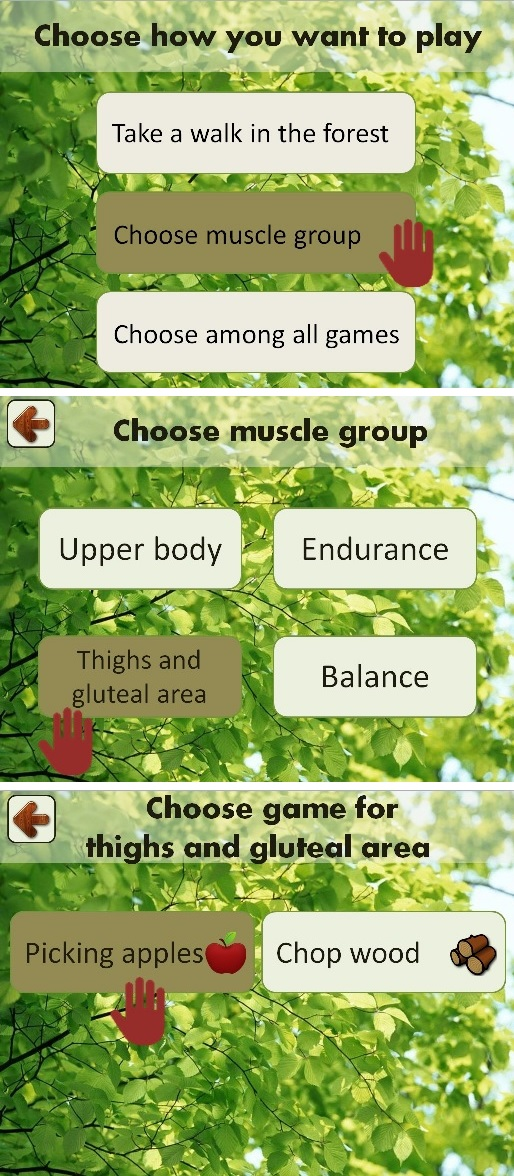
\includegraphics[scale=0.45]{menuEnglishStep1.jpg}
\caption[Menu review -  part one]{This figure shows the menu step by step, from the beginning to playing a single game, here picking apples. The selection of single games is a result of the chosen muscle group.}
\label{menu1}
\end{figure}

\begin{figure} [H]
\centering
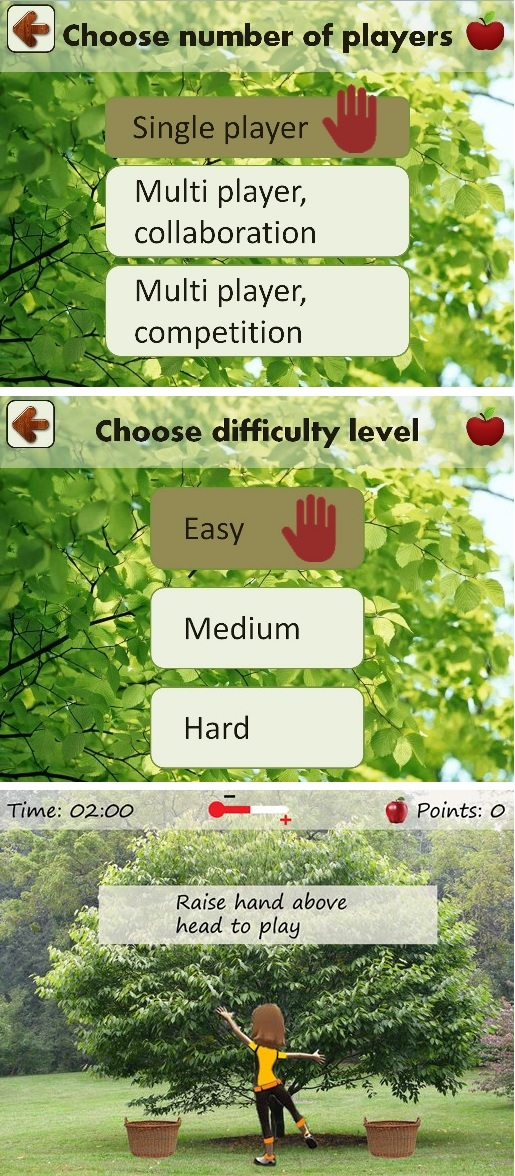
\includegraphics[scale=0.45]{menuEnglishStep2.jpg}
\caption[Menu review - part two]{This figure shows the menu step by step, from the beginning to playing a single game, here picking apples. Single player game and difficulty level easy are chosen. When ready to start the text "raise hand above head to play" is shown.}
\label{menu2}
\end{figure}

In the menu, we have used a range of green colors, and a picture of green leaves as background, to create a theme related to forest and nature. Menu buttons are arranged as list elements or in a square, depending on what is most appropriate. This is decided by the number of elements in each step; for an odd number of elements, list view is used, while square arrangement is used for an even number of elements. The size of the elements are chosen with usability in mind; there should be room for a proper font size, and it should be easy to push the right button [req. 2.12]. The buttons have a light green, almost white, background color, with a darker green outline. The text is written in black with an easy-to-read, sans serif font [req. 2.14]. The choice of background and text color is to create maximum contrast [req. 2.15]. Taking the element's surroundings into account when choosing colours is important, if you want to make the element stand out. With e.g. green vegetation as surroundings, white background color, with black, dark green, or dark blue text should be chosen to create maximum contrast [req. 2.16]. 

\begin{figure} [H]
\centering
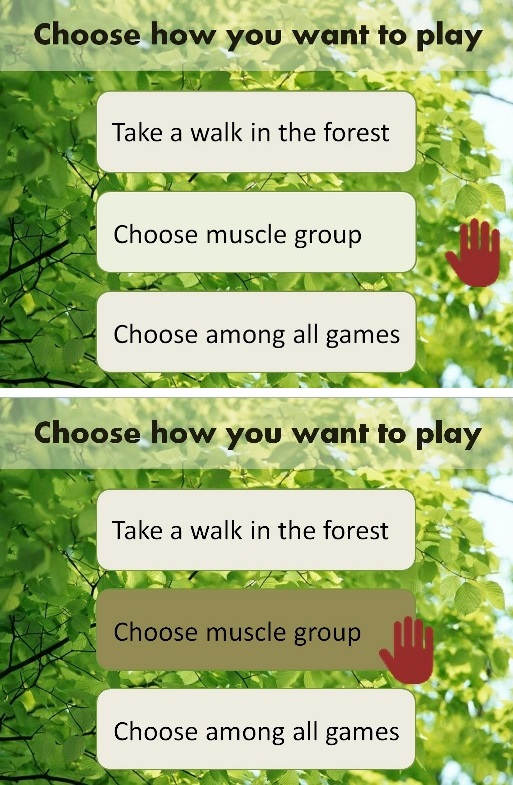
\includegraphics[scale=0.5]{menuAction.jpg}
\caption[Menu - Action and response]{In this figure an avatar hand is shown. The avatar hand will react according to the player's movements. We see that when the player move their arm over an element, it will change color.}
\label{fig:avatarAction}
\end{figure} 

The title on each step is written in a bold, black, easy to read font, on a semi-transparent light-colored background. The title is stating what choice to be made at the current step [req. 2.6]. We know from the previous chapters that it is important to have an interface with visible information, and that users always should be given feedback on their actions. Also, the informants in workshop 1 expressed that, it was general desire to see a more clear response on their actions. We have included this in our exergame by highlighting elements that are "in action" [req. 1.15], see Figure \ref{fig:avatarAction}. The player's hand movements are portrayed on the screen as an avatar hand. The avatar hand has been given a clear color and a solid fill [req. 2.11]. This has been done to avoid having the same diffuse avatar hand as in "Your Shape Fitness Evolved 2012".  

In the menu step where the player can choose between the four single games, we have used icons in addition to text on each button, see Figure \ref{fig:velgSpill}. The icons represent the challenges in each game, and they are meant to make it easier for the player to understand the game behind the button [req. 2.6]. When choosing a game, e.g. "picking apples", the icon will follow up in the right corner, to inform the player where she is headed, and to reduce memory load [req. 1.12]. This is shown in Figure \ref{fig:iconEple}.  

\begin{figure} [H]
\centering
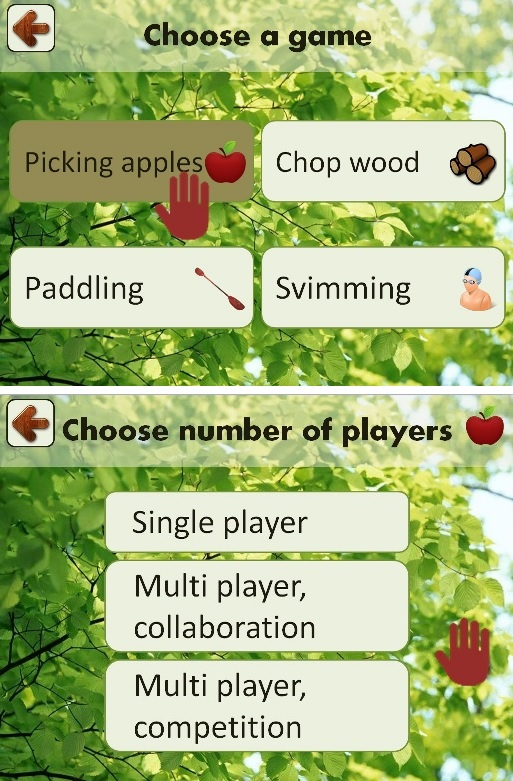
\includegraphics[scale=0.5]{menuIconApple.jpg}
\caption[Menu - use of icons]{In this figure we see that icons from the menu buttons will follow through the menu. Here we see that the apple icon will follow into the menu step where number of players are to be chosen.}
\label{fig:iconEple}
\end{figure} 

Up in the left corner there is a back button, which will make it possible for users to always regret their action [req. 1.30]. The back button is shaped and coloured similar to the other menu buttons to maintain consistency and intuitiveness [req. 2.6-7]. The choice of placement is bases on the natural way to read and observe information, which is from top to bottom, from left to right. The navigation should therefore be on top. We avoided placing the back button in the bottom left corner to not mix it with the cancel/pause feature included in the Kinect software (holding your left hand straight 45 degrees from your body). The back button is marked with a wooden arrow, a familiar and intuitive icon related to navigation. The choice of using an wooden arrow is based on its relation to the forest theme. 
     
\section{A Video Game Series}
"Out in the Nature" is part of an exergame series called "Kinect Experiences". This series consist of 4 individual games with the same structure as the game we have already presented. This means, one compounded game and four single games. The difference between the exergames is the main themes. In addition to "Out in the Nature", the "Kinect Experience" series consist of the exergames "Farm Life", "On Vacation" and "In the Mountains". The five games within each exergame will consist of activities that are connected to the main theme of each video game, like the exergame we already have presented. Examples of single games can be gathering eggs, and stacking hay bales in "Farm Life", and a walk on the beach, or catching gold fish with a hoof in "On Vacation". The idea behind this video game series is to offer a wide range of games, activities and exercises that fits the various interests the user group have [req. 1.2, 1.4-5]. What this video game series would look like is shown in Figure \ref{fig:videogameseriesAlone}. 

\begin{figure} [H]
\centering
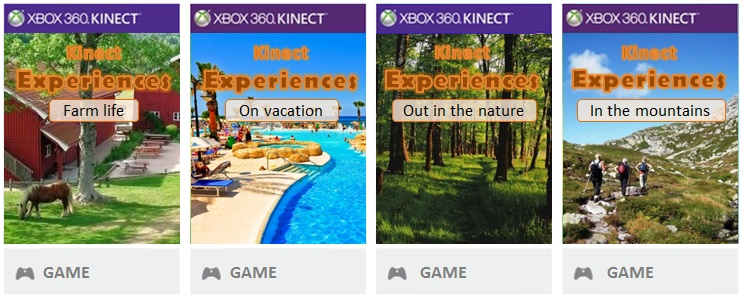
\includegraphics[scale=0.65]{videoGameSeriesAlone.jpg}
\caption[Presentation of our video game series]{A presentation of our video game series "Kinect Experiences" [modified from \cite{XboxNettside}].}
\label{fig:videogameseriesAlone}
\end{figure}


\cleardoublepage
\chapter{Findings from Workshop 2}
\label{chap:findW2}

In workshop 2 we wanted to evaluate the design against requirements, in line with on of the activities of user centered design, depicted in Figure \ref{userdesign}. A description of the execution of this workshop can be found in Section \ref{sec:ws2}. In this chapter we will present the findings from the workshop. The presented findings are based upon feedback from the informants, and our perception of their reactions to the presentation. The five informants are referred to by using I1 to I5, and are randomised so there is no relation to the references in workshop 1. Due to requirements to anonymity we have decided to not distinguish between male and female. Therefore, we refer to all the informants as females.  Quotes are translated from Norwegian to English to  preserve the meaning. 

\section{The Games}

\subsection{Game 1: Nature Trail with Quizzes}

When we presented our "Nature Trail" concept it took some time before the informants came with comments. It appeared that it was not clear to them from the pictures how this game really would work. \emph{"[...] It is impossible for me to say anything now about what I think about this. This is because I do not have a sense of how it works"}, I4 said. She continued with, \emph{"Can I ask, this lady, or the girl [on the screen], if I do like this [making movements with her upper body], then she would do the same?"}.  It seemed that the participants understood more about how the game would work, after we confirmed this, and more comments appeared. I3 said, \emph{"I think this was a good idea because the environment you are in is familiar to me"}. The other informants agreed. Several times during the discussion I1 said that she thought the concept was very nice. \emph{This was very nice"}, she said, while I4 followed with \emph{"fun development"}.  

About having quizzes in the nature trail, I1 was very sceptical. She was afraid that it would draw attention away from the physical tasks. I3 agreed and said \emph{"It will become a sort of test on how good you are [at answering questions in a quiz], and that is not the way I have understood the point about these games"}. I1 meant strongly that we should separate the quizzes from the rest of the game. She said \emph{"I think this is very nice. [...] However, I think you should think very thoroughly about the cognitive, about the questions linked with the physical. You need to have a purpose about it, a goal on what you want to achieve"}. 

It was not clear for all the informants when the quizzes would appear in the nature trail. They all seemed to believe that they would appear at the same time as they were doing something else, like while balancing over a log. To be able to focus on both the physical challenges and the quiz, I4 suggested that these questions should appear somewhere where it was natural to take a break, and that the player should be able to sit down and answer the questions. I4 also proposed that the player could get to see the questions before the game started, and then answer them after a while. Her experience was that if she was thinking about something, the answer usually came up eventually. 

From the discussion we understood that there were confusion about the link between the cognitive and physical challenges. This was not only about the goal of having a quiz, but also the quiz's purpose in the game. \emph{"The points [shown in the top part of the screen] do you get them just if you manage the questions? It does not have anything to do with the [physical] skills?"}, I2 asked. Several of the informants wondered about how the question allocation would work. \emph{"When I'm doing the game time number three, will it still be the same assignments that appears?"}. I4 also asked if the player could choose category for the questions.  

The informants were mostly concerned about doing two things at the same time, like answering questions at the same time as doing an exercise. Another challenge they commented on was the one where they were suppose to balance over a log. I1 said \emph{"This exercises your balance, right, so it is easy to fall yourself, if you get [takes her hand to her head as a sign of getting dizzy]"}, referring to the possibility of falling not only in the game, but also in real life. There were also some technical questions about this challenge. \emph{"If I am balancing on the log, and I fall down, would I feel that? If I did not manage to keep the balance, and fell in the water?"}, I4 asked. 

Most of the elements in the game environment were familiar to the informants. However, the heart was not that obvious. \emph{"I did not quite understand. The heart that are floating there [points at the screen], is the idea that you should take it?"}, I4 asked. I2 followed with \emph{"If you get the heart, does it disappear?"}. Further the informants wondered where the number of gathered hearts will be shown on the screen. We explained that to limit the information on the screen the hearts will only fill the "health bar", as an indication of good health. They understood, and agreed that it would be hard to count the number of hearts on the screen, and that the "health bar" was a good idea. Not all of the informants were positive about the hearts. \emph{"But hearts.. It is a little feminine"}, said I1, and suggested that maybe hunting butterflies would be better, especially for men because it could trigger the hunting instinct. I3 joked \emph{"A bottle of beer?"}, while I4 adds \emph{"Lets see.. A feather? Flying by?"}. 

At first the informants did not understand how the different difficult levels would work. I1 said that she would not be forced into something she would not do, and that she wanted to be able to choose which difficulty level to play in. \emph{"I am thinking that I do not want to get forced into something that is hard, that I do not master. Because then I get mad"}, she said. We explained how the game will remember the players progress and adjust difficulty level accordingly, and that there also will be initial difficulty levels that the player can choose between. She agreed that this was a nice way to do it, as long as she had the possibility to choose herself. I4 also agreed on the way we had organised the different levels. \emph{"I think it is an advantage that everyone starts at the easy level, and the more confident you get, the harder it gets. I think that is a good way to control"}.

\subsection{Game 2: Picking Apples}

The informants all seemed to like the picking apple game. \emph{"I think this was nice"} I3 said. However, there were some concerns related to how the apples would appear, and how they could plan the apple picking. I4 said \emph{"I feel that two apples is fast to gather. If the tree was full of apples I would be more eager to play. [...] It might be weird if they should pop up all the time"}. We explained that the apples appear randomly because of both the cognitive and physical exercise. They all agreed that this was a nice solution. 


\section{Information, Instructions, and the Menu}

More information and instructions were stated as important in workshop 1, and we had therefore tried to include this in our exergame concept. The informants seemed satisfied with the way we had presented this, and they also seemed to recognise the included instructions inspired by the sports game, like "raise hand above head to play". We asked if they noticed the arrow in the upper left corner, and I5 immediately said \emph{"back"}. Everyone agreed that it was clear that the arrow indicated a back-button. About the combination of colors and how the pictures looked in general, I1 said \emph{"beautiful!"}. I3 mentioned that it would be better with more shadow around the buttons, to indicate that it actually is a button. On the questions on whether there were too many steps in the menu before you could start the game, the only comment was from I1, who said \emph{"[...] When you have used the menu, then you want to have shortcuts"}. 

When we presented the possibility to choose game play based on muscle groups, there arose many questions on what we meant about the term "muscle group". It became clear that we had been inconsistent with this categorisation. I5 said \emph{"[...] When you use the term muscle group, then I think that endurance do not fit under this term"}.   

All of the informants had some problems understanding the different difficulty levels in the games. \emph{"I had an immediate reaction when I saw this [points on the screen that shows the three different forests with different difficulty levels], that it took me some time before I could see that these different environments [the different forests] represents different difficulty levels"}, I3 said. The other informants agreed. Further I3 suggested, \emph{"Easy forest, medium forest, hard forest, or what you would call it"}. About the different difficulty levels, some of the informants wondered if the same challenges would appear in all levels, just more frequently. This was the way we have thought the game to be.

\section{Music and Atmosphere}

The informants were curious about what kind of music the games would get. I4 asked \emph{"I am wondering about the atmosphere and environment. When I am balancing there [on the log], will I hear the sound of water?"}. We explained that we wanted to include sounds that are natural to the environment. I2 said \emph{"Not noisy, like last time [referring to the music in the games played in workshop 1]"}. We told them that we want to use peaceful music, like classical music. I1 suggested \emph{"You should think about rhythmic music. Maybe it is just as easy to pick apples to a rhythm, instead of picking as many as possible? [...] Then, when the apples ripens, it will be according to the rhythm"}. 

\section{The Delay Problem}


One of the informants remembered the technical aspects related to the delay from the last workshop. She said  \emph{"this is a technical question which is about the capacity in the computing system. It is not straightforward to solve technically. [...] Do you have any thoughts about this?"}. The informants were aware that this was beyond the scope of our thesis, but we informed them that we will look into the delay problem.

\section{Informants Showing General Interest in the Games}

Some of the informants were concerned about getting tired of the game after playing it several times. One informant asked if it would be possible to exchange the game if it got boring. We presented our idea for a video game series, where each game could be downloaded from the Internet for a small amount of money, in this case 99 NOK (about 18 USD). The informants stated that this was an affordable price. They showed interest and curiosity about how they could get the game. I1 asked \emph{"Do you think you could get it on prescription?"}, and I4 continues by asking if it would be possible to rent a game like this from the library. When discussing the exchange of games if they got bored, I3 expressed that she did not think this would be a problem. \emph{"[...] I would think that when I have completed the game I have exercised, and that it would be satisfactory for me. And then I could easily do it over again"}. After I3 had put it that way, the other informants seemed to agree.

All of the informants were eager to hear more about the development of this exergame, and they wanted to get information about when the game would appeared on the market. I4 said \emph{"It would have been fun to know when it comes. I have faith in this project"}. \emph{"Include us in the customer list!"}, I1 laughed.




\cleardoublepage
\chapter{Discussion}
\label{chap:discussion}

\section{Discussion of Findings from Workshop 1}

In Section 6.1. we discussed the importance of usability which is about how easy a system is to use, learn and understand. Workshop 1 was performed to see how a set of relevant users interacted with existing commercial exergames, and to identify what aspects of these games work and do not work. \cite{usabilitydef} states three relevant elements that can say something about a system's usability: \emph{effectiveness}, \emph{efficiency}  and \emph{satisfaction}. These were aspects among others that we tried to measure in the workshop. We also tried to answer the concept \emph{context of use}. We wanted to discover the needs of the games' intended users, the needs for the functionality and the environment for the game. Where and in what circumstances the game can be used, was discussed in our previous project assignment \cite{project}. This is not our main focus in this thesis, but will briefly be discussed in Chapter \ref{subsec:whatwhere} 

In this section, we will discuss the findings from workshop 1 and relate these findings to the literature provided in precious chapters. In workshop 1, and in our literature study we have tried to answer these research questions: 

\emph{RQ1: Are existing commercial Xbox Kinect games suitable for exercising purpose for the senior user group?}

\emph{RQ2: What are the design challenges when developing video games aimed for exercising for the senior user group?}

First, we will provide a general discussion, and then we will summarize by more precisely answer the two questions at the end of this section. 

\subsection{Control of Character, Clear Goals and Feedback}
In the Game Flow model \cite{sweetser} discussed in Chapter \ref{sec:heur}. eight core elements that should be present to experience enjoyment in games are described. Of these eight core elements we found a lack of three of the elements in the commercial games tested in workshop 1. The informants expressed that they did not feel that they had control over their character. This was due to the significant delay that was present in the games. In addition it came clear from the observation that it was not always easy to understand when the game started and ended, as well as what was an instruction video and what was the actual game. The element clear goals did also seem to lack in the commercial games, and it was expressed by one of the informants that there was a need for more instructions on what was actually expected from them and the rules of the game. The last element the informants were not satisfied with was the feedback. Also two of the eight golden \cite{mmi} rules presented in Chapter \ref{subsec:golden} discuss the importance of getting informative feedback at appropriate time. The informants desired more feedback on their actions, and they especially wanted to know whether they did the exercises right or wrong. They did not feel that they got this feedback in the games played in the workshop, which made them both confused and frustrated at times. Clear goals, appropriate instruction, information and feedback, are aspects highly considered in the new game concept. The delay problematic will be discussed in more detail in Section \ref{sec:delay}.
 
\subsection{Immersion and Concentration}
As presented in the GameFlow model \cite{sweetser} immersion and concentration are important aspects of the gaming experience. It was hard to evaluate from observing and interviewing informants if they were immersed into the game and concentrated on the tasks. However, comments like \emph{"I felt like the person [avatar] itself"}, and cheerful comments given by the informants while they played, like \emph{"I wanted that pineapple"}, suggested that the informants immersed into the game. If we are to evaluate, we would say that all the games required concentration to perform the tasks right. However, it did not always seem like the informants were that concentrated. One example of this is that sometimes we had to assist in reading the messages appearing on the screen, like "raise hand above head to play", while they read the same type of messages themselves at other times. We believe that the text should have been clear enough, and that the reason for them not reading the text, was because they were not concentrated enough on the game. 

\subsection{The Possibility to Customise}
As mentioned, in our previous project \cite{project} we evaluated the game to fit as a tool that physiotherapists can use as an alternative exercise method for their patients. The value proposition of this game we described as: \emph{"A tool with the ability to customize an exercise program, and to offer an alternative, fun and motivating training method, while at the same time ease the workload of the physiotherapist"} \cite{project}. In this thesis we have focused on one part, of this description: \emph{an alternative, fun and motivating training method}. For this game to meet these three criteria, the end-users had to be included in the development process. However, as learned from \cite{Billis}, \cite{gregor}, \cite{gerling1}, as well as from the informants, there is a need to customise these kind of games and acknowledge elderly's various limitations and disabilities. One example given by the informants was that the skiing game could have too fast pace for some people within this user group, and that it could cause problems for people with decline in their balance function. The possibility to customize the games can for example be a feature in the physiotherapists interface, where they can put together different exercises within the game story, that fits their patient. Another example is for the user herself to have an interface where she can put together her own program.  As can be found in Table \ref{tab:func2} in Chapter \ref{sec:req} we have made additional requirements for this, but we have limited our thesis to not prototype a user-interface for this. 

\subsection{Aspects to Meet Player Enjoyment}
In Chapter \ref{sec:motivators} we discussed self-efficacy as an important determinant of exercise behaviour. Elements that are relevant to sustain this exercise behaviour are the feeling of pleasure and satisfaction, and self-regulatory skills. This was also discussed in workshop 1 as important aspects, and the informants mentioned goal setting, the possibility for socialising, and the possibility to self decide what to do, as important. The feeling of mastery was seen as significant. They were clear that if they did not get the feeling of mastery, they would not play these games. This relates to the elements discussed in the Game Flow model \cite{sweetser}, where some of the criteria for player enjoyment in games are to include challenges that match the player's skill level, to have different levels of challenges, and clear goals. In addition, the Game Flow model says that games should support social interaction. Also in Chapter \ref{sec:exergames} the importance of social interaction in exergames are discussed, and  as much as 62 percent of all gamers say they play with others \cite{statistics2012}. Several previous studies \cite{Billis}, \cite{gerling2}, \cite{gerling1} discussed in Chapter \ref{sec:summaryguidelines} also stress the importance of the social factors of a game. Offering social interaction, can especially be important for elderly who experience loneliness in their everyday life, due to inactivity \cite{project}. It was interesting to learn that social interaction also was seen as important by the informants. The majority of the informants would rather play together than alone. However, none of the informants could see themselves playing together with others over the internet. This relates to the findings done in \cite{Gajadhar} where it was shown that elderly enjoyed playing together in the same room more than playing online. We also believe that one of the reasons for the informants stating this was because they did not understand the concept of "playing over the internet", as a result of their inexperience with this kind of technology as discussed in Chapter \ref{subsec:characteristics}. This might indicate that the market is too immature for this. When it comes to social interaction, one of the informants meant it was more motivating to cooperate than compete. This was also found in \cite{Gajadhar} where they in line with the result from their study and from previous studies conclude that the focus should be on cooperative play rather than competition for this group of people. 

The informants' opinions did not differ much according to gender on what they liked and did not like in the games we tested. However, as discussed in Chapter \ref{sec:motivators} different people's needs and expectations, as well as aspects such as gender and ethnicity should be considered. We will meet this by making a concept with a series of games that covers a variety of interests, as well as getting to choose a man character or a woman character. Race might also be considered, but it is difficult to cover all races. Chao et al. \cite{chao} discuss that to meet these requirements it is important to be in contact with the relevant people. Even though we clearly have not covered the total group of elderly, we have included a small group to understand some needs and expectations. In Chapter \ref{sec:sergames} we discussed how video games can function as a pedagogical tool and it was shown that important factors to focus on includes motivation, effectiveness and intuitiveness. Another aspect discussed in the same chapter is behaviourism, which states that if someone is rewarded for something he or she is likely to repeat the action that triggered the reward KILDE. These aspects were also mentioned by the informants, who stated that the system needs to be easy to understand, and that the feeling of mastery and that you learn something are important.  One informant mentioned that if they did not manage to do something, they would stop doing it. In our game concept we will focus on emphasising the goals in the game, and the player will be rewarded with points. In addition we provide different levels. This will be done in two ways: Different initial difficulty levels the player can choose between, and different difficulty levels within the initial levels, where the next level depends on the previous.  

\subsection{Appropriate and Simple Feedback and Information}
In Chapter \ref{sec:summaryguidelines} we listed typical characteristics of elderly based on findings from the literature. In our research we had a group of informants, who were relatively physically and mentally fit. From the list provided in Chapter \ref{sec:summaryguidelines} we only experiences three out of the nine characteristics. We experienced that one of the informants had problems reading the text in some of the menus. Because there was only one informant that seemed to have problems with this, we assume that this informant might have had impaired vision. However, it is important to acknowledge that impaired vision is a common problem for the older population as discussed in Chapter \ref{sec:summaryguidelines}, and in Chapter \ref{sec:designelderly}, and it should therefore be considered in a game designed for this group. The group of informants had interest in technology and used different types of technology, like computer, tablets, mobile phones, e-mail, e-banking, TV, etc. However, none of the informants had any experience with video games. In the beginning of the workshop we experienced that some of the informants were insecure, and had problems understanding what they were suppose to do. It took some time for most of them to understand that they had to use their body to play. Therefore, we see a need for clearer instructions both before and under game play. This includes an introduction to how the system works, like how to interact with the sensor. The last of the characteristics listed in Chapter \ref{sec:summaryguidelines}  we experienced, was that some of the informants expressed that it was hard to do more than one thing at the same time. Therefore, the information given, and the tasks to be done, should be limited, and adjustable. The possibility to add more functionality after the existing functionalities are managed was suggested by one informant. This is also listed as one of the guidelines in Chapter \ref{sec:summaryguidelines}, and suits well with the requirements of simplicity discussed in Chapter \ref{sec:simplicity}. 

In Chapter \ref{sec:summaryguidelines} we presented a set of previous studies and provided a summary of some important aspects that can serve as guidelines when developing games for elderly. One of these guidelines suggested in \cite{Billis} and \cite{gerling1} is about giving motivating feedback. Some of the games that were played in workshop 1 had a lot of different features that were suppose to be motivating. However, by some of the informants this was rather seen as annoying.  In addition the amount of the information given, both text and audio, was experienced as too much. At the same time, some of the informants stated that they did not recognize these type of messages at all. In Chapter \ref{sec:simplicity} we discuss minimalistic design which is about bringing the most important elements into focus, without elements that will distract the user. Microsoft presents it as "Simple Can Be Powerful", which means that simplistic design not necessarily needs to mean lack of functionality. From this we conclude that we should avoid too much features in our video game concept. We should keep it simple, and focus on a few motivating aspects. One of the informants desired more time to read information and instructions, and suggested that there should be a way to tell the system when you are finished reading. This is also a requirement suggested in \cite{w3cTekst} which we have included in the guidelines for making user-friendly interfaces for elderly in Chapter \ref{sec:designelderly}, and will be taken into account in our game concept. 

\subsection{Cultural and Lifestyle Diversity}
Another guideline discussed in Chapter \ref{sec:summaryguidelines}, and the second of the eight golden rules presented in Chapter \ref{subsec:golden}, are about matching cultural and lifestyle diversity in the games. This was expressed by the informants as important, and they suggested different type of themes for a possible game concept, like dance, swimming, apple picking etc.. If they were to play a game like this they stated that it would need to include sports or activities related to real life. They also mentioned the importance of appropriate music. They did not like the music in the commercial games because they were not the type of music they used to listen to. Using appropriate music was also discussed in Chapter \ref{sec:motivators}, and \cite{schutzer} sees music also as a way to divert from pain coming from the exercises. The majority of the informants agreed that music was important, especially to keep the rhythm. However, they stated that they wanted it quite, and they wanted music more related to their generation. This is an important requirement we will set for the exergame, however, it is without our profession to say anything specific about what music to include. 

\subsection{Summary}
We will now provide a summary of the discussion to in a more precise way answer research questions 1 and 2. 

\emph{RQ1: Are existing commercial Xbox Kinect games suitable for exercising purpose for the senior user group?}

As mentioned initially, effectiveness, efficiency  and satisfaction are relevant measurements when evaluating the usability of systems. From findings done in workshop 1 we can conclude the following about the commercial games tested: 
\begin{itemize}
\renewcommand{\labelitemi}{$\bullet$}
\item The existing commercial games tested on a group of elderly do not meet the requirements of effectiveness. The games do not spend enough time on instructions and information, and do not give sufficient feedback on what the players are doing is right. The menus are too complicated and it is too many elements showing at the same time. The buttons presented in the games are too sensitive, and it is not intuitive how to press the buttons. 
\item The existing games meet only to a degree the requirement of efficiency. In FruitNinja it was clear that the informants did not understand what was required from them, and they just waved their hands uncontrollably. The majority of the the informants understood what was expected from them in the tennis game, and played through this game without problems. The skiing game was also well understood, until the second match where the two players that played together switched tracks. All of the informants had problems relating to their player after switching tracks. None of the menus met the requirements of efficiency. We had to assist the informants through the menus, and because of too much information and too sensitive buttons, the informants spend unnecessary time on getting through the menus.
\item Two of the four games played in workshop 1 meet the requirement of satisfaction. All of the informants liked playing the tennis and skiing game and they had fun while playing. FruitNinja, they did not like that much, which relates to their wish for playing games with a meaningful content that they could relate to everyday life, which is not the case for FruitNinja. The informants were not satisfied with the personal trainer game either, because this focused on "just" regular training, which they would rather do without the game. This strengthens up under Michael Zyda's statement on that the main focus in serious games should be fun and entertainment \cite{zyda2005visual}. 
\end{itemize}

It is important to mention that this was the first time the informants played games like these, and initially they did only play the games once \footnote{Three of the informants got to play the skiing game a second time because they specifically asked for it. We did not observe anything new in this second session, and have because of this, and because the rest of the informants did not try a second time, not included this in our analysis}, which did not enable us to say anything about the informants learning curve. However, we did see that they understood more what was expected from them, and that they got more confident after a while. If we had went on with several rounds with the same games, we might have seen improvements. This was also mentioned by the informants. 

\emph{RQ2: What are the design challenges when developing video games aimed for exercising for the senior user group?}

It is important that we acknowledge the difficulties about engaging a user group into a setting they are completely unfamiliar with. It is hard to evaluate some users needs, when they do not even know about these needs themselves. We have learned from workshop 1 and from our previous project that today's elderly are not necessarily the right user group for a game like this, but that the next generation of elderly are more suitable. However, it is hard to test a tool that is meant as an alternative form for exercising on people who are physically in good shape, and who keep one doing regular exercising. 

The game should meet the requirements from the GameFlow model \cite{sweetser} that we discused to be inportant in Chapter \ref{sec:heur}. We found this model to serve as good guidelines, as many of them was mentioned as important aspects by the informants, and also because there is a clear relation between these guidelines and the guidelines we can draw out from the literature, presented in the previous chapters. Specifically the informants desired a game with a story that appeals and relates to real life, as well as appropriate music to their age. It was urged for more instructions on how to interact with the game, as well as what was expected from the players, the goals, and the rewards. The menus in the commercial games were seen as challenging because of the amount of information and the sensitive buttons. In a game for this user group this needs to be improved. The majority of the informants would only play these type of games together with others. In \cite{chao}, \cite{statistics2012}, \cite{Billis}, \cite{gerling2} and \cite{gerling1} social aspects are also discussed to be important, as well as it is a recommended guideline in the Game Flow model \cite{sweetser}. Therefore, it is important to include this in our game concept. The delay in the games was seen as a big problem, and should be acknowledged.  This is a technical issue that we are not in the position to evaluate the reason for. We believe that if this game is to be used for exercising, both at home and in clinical settings, technical precision have to be present. 

\section{Discussion of Findings from Workshop 2}
In Section \ref{sec:userinvolvement} we presented how important user involvement is during system development, as the end-users are the ones who will use the final product, and are the only ones who know what they want. After making a concept based on theory, previous studies, and findings from workshop 1, we wanted to invite elderly to a second workshop to get feedback on our ideas and design proposals. In workshop 2 we presented our prototypes for a exergame concept for elderly, and we had questions and discussions during the presentation. Figure \ref{userdesign}, from ISO 13407, is a cycle of four steps for user centered design, where workshop 2 is about the fourth step, evaluating system design. Involving the end-user in the design process will increase the possibility of making a user-friendly interface for the intended user group, which is stated in Section \ref{sec:usability} as crucial for making a successful system. Feedback from workshop 2 will be discussed, and we will present important aspects to be included in the future work of designing an exergame for elderly. These aspects will just be discussed, we will not make any changes to our current exergame concept, as this is out of the scope of this thesis.

In addition to discussing findings from workshop, and relating them to theory provided in previous chapters, we will try to answer this research question:
 
\emph{RQ4: Is it possible in an early development phase to involve a user group that is inexperienced with the type of technology being developed?}

We will start with a general discussion, and then try to answer this research question in the summary of this section. 

\subsection{Difficulty Levels}

Mostly, the informants liked the exergame concept we presented for them, but there were some concerns and uncertainties about integrating quizzes in the trail. The GameFlow model, presented in Section \ref{sec:heur}, consist of eight core elements, where concentration is one of these elements. Here, the importance of not distracting players from tasks the want or need to concentrate on, is emphasised. In addition, players should not be bothered with tasks they see as important. The informants expressed concerns about having quizzes together with physical tasks, as they felt that might draw attention away from one of them. They did not like the idea of doing two thing as the same time. This would be important to take into consideration when developing an exergame for elderly, as it is a fact that this group of people have difficulties doing more than one thing at the same time \cite{bruin}. This was mentioned when showing prototypes, where the players were suppose to do some kind of task, and at the same time collecting hearts and answering questions. We suggest that one solution for future work could be to choose, when starting up the game, whether you want to include the cognitive challenges or not. 

From the Challenge element in the GameFlow model we know that games should offer difficulty levels that matches the player's skills. This, combined with the Concentration element, has lead to the idea of adjusting frequency between the appearance of obstacles and number of simultaneous tasks will be according to the various difficulty levels. The difficulty of required exercises and movement should also be controlled by the difficulty level, as this is an important feature for elderly that might suffer from various physical challenges \cite{gregor}, \cite{gerling1}. Some challenges, like balancing over a log, was mentioned as a bit challenging. One informant stated that she though she would feel dizzy, and that she was afraid of falling (in real-life). This challenge was also reviewed by a physiotherapist (NINA). She stated that it was a difficult exercise to perform, and therefore should be included in higher levels in the game. This support the importance of providing the possibility for players to choose difficulty levels themselves \cite{gregor}, \cite{gerling1}. However, the GameFlow model emphasises that the game also should support adjustment of difficult level after the player's skills and progress. By offering both these opportunities in this exergame, we meet the feedback from the informants, as they want to be able to master the various tasks, and not be forced into something they would not master. They both wanted to choose themselves, and to let the game follow their increased skills. 

\subsection{Graphics, Sounds and Interface}

As mentioned in the GameFlow theory, immersion is an important aspect for the player to effortless be involved in the game \cite{sweetser}. In workshop 2 the informants expressed that the concept with the nature trail was a good idea because they were familiar with the environment. This supports findings from previous studies, like in \cite{gerling2}, where the participants appreciated the use of a real-life environment.  

The summary guidelines presented in Section \ref{subsec:guidelines} emphasises that an interface should be simple and not to complex, and that important elements should be brought into focus. The informants seemed to like and understand the menu interface we presented for them. Their general perception of the interface was that is was \emph{"beautiful"}. The back-button and the purpose of it was observed and understood immediately. A comment was to highlight the buttons even more, making them stand out more with a hint of shadow around them. SilverPromenade, presented in Section [EGENTLIG ANNEN REFERANSE] \ref{chap:exforseniors}, had success with an intuitive and user-friendly interface, which quickly and easily guided the users to game play. As mentioned in \ref{sec:menu}, we have a longer menu to include the possibility to choose actions, and at the same time avoid too much information at each step. The informants feedback was that they felt the menu was OK, but that they wanted to use shortcuts when they had got familiar with the game. Inclusion of shortcuts for the experienced user is mentioned as an important feature in the second of the Eight Golden Rules, presented in \ref{subsec:golden}.

From \cite{schutzer} and Section \ref{sec:georep}, we know that sound and music is an important part of the players enjoyment and gaming experience. We did not present any music, or soundtrack, for the elderly, as this, as mentioned in Section \ref{sec:outinthenature}, is out of our competence area. However, we told the informants that we wanted to use calm and peaceful music, like classical music. This to meet their feedback from workshop 1, where they expressed that it was too much noise. We also presented the informants for ambient effects, like birdsong and sound of running water, as this are sound related to the environment of the game, and sound effects like a "ping" when collecting a heart. They seemed OK with this music and sound, but they wanted something with rhythm to more easily immerse into the game and exercise. Future work would therefore be to find appropriate music for the nature trail and the single games, based on the exercise and pace in each game. 

Generally, there were a lot of questions related to game play and the various elements in the prototypes. An example of this was the question on what the hearts meant, and what would happen if they touched them. That the hearts were observed quickly is positive, as these are important elements of the game. This means that they stand out, which is stated as important in Section \ref{sec:designelderly} and \ref{subsec:guidelines}. In the same sections, intuitive interfaces is stated as important. What is not so positive with all the questions, is that it states that our interfaces are not that intuitive as we had believed. This has to be taken into consideration for future work. Two elements in the menu were a source to a lot of discussion due to lack of intuitiveness and consistency. One of these was the menu step where the player was to choose environment and difficulty level. This especially yield the understanding of the increased difficulty level between the three environments. It came clear to us that it was not very intuitive that the three different forests we presented in the menu were meant as three different difficulty levels. Future work would be to focus on including textual information to make this part more intuitive. A suggestion would also be to have instructions on what the different difficulty level means.

The other menu step was where the player had chosen to play according to a specific muscle group. The informants did not see consistency between the term "muscle group" and what we presented in the menu. I1 said \emph{"Yes, muscle group, it does not fit with what you show here [refers to the picture of the menu where the player can choose different type of muscle groups]"}. This is not positive for our interface, as consistency is mentioned in the first of the Eight Golden Rules. We acknowledge that we had not thought through this step in the menu thoroughly. However, we concluded that this is future work for professionals, like a physiotherapist, to do, and that what we presented was just an example. 

As we saw from the findings from workshop 2, the informants had questions about what would happen if they were to fall down from the log and into the river. Similar technical issues could include the possibility to walk outside the path and into the forest. These kind of limitations that have to be programmed into the game, are aspect we have not considered in our concept. However, it is something that needs to be looked further into and integrated into the system requirements.   

\subsection{Few Comments and Moderate Response}
As mentioned, there were a lot of questions from the informants, but what was more common during workshop 2 was that there was no comments at all. When we presented the various prototypes, the informants responded with silently nodding or just looking mutely at the screen. There could be several reasons for this. One reason could be because of the informants lack of experience with this type of technology and video games in general. This makes it difficult to comment on a video game concept, as they do not know what to look for and respond to. One of the informants stated that it was impossible for her to say something about our exergame concept, as she did not know anything about how the game would work. Another reason could be related to how we presented our prototypes. The exergame we have made a concept for is based on highly interactive video game technology, and as presented in \ref{sec:prototypes}, it is therefore very difficult to make good prototypes. In addition, we did not make the prototypes in a way where it was possible for the informants to interact with the prototypes. We presented the prototypes with the "Wizard of Oz", with the informants observing. 

The lack of interaction between the informants and the prototype could have lead to poor understanding of how the game would work. A question from one informant supports this assumption. She asked if the girl in the prototype would respond to her movements, even though she had played games like this before. A final reason could be that we did not present the information good enough. After the question from the informant about the avatar, we explained how it worked, and it seemed that the informants understood quickly. This increased understanding lead to more questions and feedback. Also, when I4 described the quiz as she would like to have it, we realized that this was the same way we had imagined it to be. It seemed that we did not present this clear enough, as there was never meant to be the way in which they would have to answer a question at the same time as they were balancing over the log, like I4 thought.   

\subsection{Summary}
We will now provide a summary of the discussion of findings from workshop 2, where we will draw important aspects to consider in the future work of the development of an exergame for elderly. We will also try to answer research question 4.

\textbf{Future Work for an Exergame for Elderly}
\begin{itemize}
\renewcommand{\labelitemi}{$\bullet$}
\item Future work should include working on how to present the idea of difficulty levels for the users. There were a lot of questions and confusion related to what each difficulty level implied, and also how the difficulty levels were chosen. When we explained how it would work, the informants liked the idea, but this did not came clear from our prototyped concept. Future work should focus on including instructions and information about how the difficulty level is chosen and controlled. In addition, textual information should be included in the menu step where the player is to choose environment, to indicate that each environment holds different difficulty levels.  
\item Our prototypes showed obstacles, hearts and quiz icons all in the same picture. We presented it this way to show how elements will appear along the way in the nature trail, but the informants did not see the depth in the picture, and believed that they were suppose to do everything at the same time. The elements shown all together also made the prototype appear as distracting, as the informants did not know what to focus on. Future work should include studying the presentation of elements. A suggestion would be to let the elements appear when the player reach a certain distance, to avoid having too much elements on the screen at the same time.
\item In future work, the exergame should hold the possibility to separate the quiz from the nature trail. This should be done to let the player more easily focus on one task at the time. It might be more natural to include the quiz when the player has gotten more familiar with the game.
\item Future work should focus on how the quizzes should work, and how and when they will appear. How we presented the prototypes, made the informants believe that they should answer quizzes while doing something else. I4 presented how she would like the quizzes to be, answering questions separate from other tasks, and this is the same way that we had imagined it to be. We clearly did not present this element good enough. This shows the need for a thorough introduction to how the quizzes will work. Future work could also include looking into presenting the quiz icons in a different way, to not take focus away from the current tasks. 
\item The buttons in the menu should be highlighted to let them stand more out. This can be done by adding some shadow around the buttons.
\item It should be the future work for professionals to find appropriate music to the game. This yield ambient effects that fit the environment, sound effects to give users feedback on actions (like when collecting a heart), and music suitable for the intensity in the game. Maybe calm and peaceful music suits the walk in the forest, while music with more rhythm fits the picking apple game. 
\item It is important to include the purpose of all important elements in the instruction video. There were a lot of questions about the hearts and their purpose, and we presented earlier that this could be a result of lack of intuitiveness. To our defence, the idea was that the purpose of the hearts should be presented in an instruction, but this was not included in our presentation. We observed how the lack of instruction created confusion, and we therefore see the importance of having these instructions.  
\item It should be the future work for professionals, like physiotherapists, to find out which muscle groups to present as choices when the player wants to play according to a specific muscle group. Our lack of knowledge in this area shone through when we presented this part, as the informants quickly commented the lack of consistency between the term "muscle group" and what we had presented as muscle groups to choose from. 
\end{itemize}

\emph{RQ4: Is it possible in an early development phase to involve a user group that is inexperienced with the type of technology being developed?}

We found it difficult to include such an inexperienced user group in an early development phase. This it not based on the fact that development is in an early stage, but that the elderly are very inexperienced and unfamiliar with the video game technology Kinect provides. The elderly did not know what to look for or respond to when prototypes were shown to them, as they could not relate to what we presented. During workshop 2, we did not get much feedback on our prototypes. This could also be a result of our presentation of prototypes. It was difficult to make interactive prototypes for such a complex and interactive system. We know from Section \ref{sec:prototypes}, that how users interact with the prototype is crucial for understanding the system. It was not possible for the informants to interact with our prototypes, which might have lead to lack of understanding. It was not easy for the inexperienced informants to come with feedback on such an interactive system, when they were presented for still pictures, even though they had played Kinect games in workshop 1. We believe that a more interactive prototype would have lead to more understanding and that it would have triggered more feedback. However, we did not have time or knowledge to develop an interactive prototype. 
 
\section{The Delay Problem}
\label{sec:delay}
Both in workshop 1 and workshop 2, there was a lot of time spent discussing and commenting technical aspects related to the delay between the player and the avatar on the screen. This problem was a source to much confusion and frustration, and it did not give the informants a real-time experience. It is important to take this into consideration when developing a new game, since the delay destroyed part of the enjoyment for game play. Control is another one of the core elements in the GameFlow model \cite{sweetser}, and a part of this is about the player being in control of their characters and movements. Feedback from the two workshops was that the informants did not felt this control, due to the delay [SITAT].  

\begin{figure} [H]
\centering
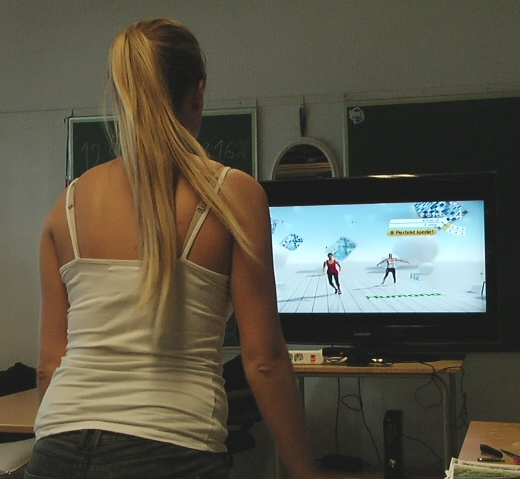
\includegraphics[scale=0.6]{kineDelay.jpg}
\caption[The Kinect sensor delay]{This figure shows that there is a clear delay between the players movements and the avatar on the screen. The avatar to the left is the trainer, while the other avatar portrays the player. We see that the player follows the trainer, having the arms down, while the avatar portraying the player has the arms straight out to the sides.}
\label{pickingapples}
\end{figure}

\section{Miscellaneous Aspects to Consider About the Exergame Concept}
\label{sec:misc}

\subsection{Discussion on where and in what circumstances the game can be used}
DENNE ER IKKE FERDIG, MEN SKAL SNAKKES LITT MER OM.
\label{subsec:whatwhere}

In our previous project \cite{project} we evaluated the game to have the most potential in a clinical setting, offered as a training method at physiotherapy clinics. This was based on two main things. First, "Samhandlingsreformen" encourage the use of welfare technology where possible in health care. Second, the majority of the senior user group, have little or no experience with video games, which will make it hard to reach out to these customers. In this thesis we have not focused on where the game should be implemented. However, we did ask the informants where they could see the game be used and two main settings were mentioned: in a group setting, for example in nursing homes, and in a setting with grandchildren. We decided to not study any further where the game can be implemented. This was both because we experienced that the majority of the informants had a hard time picturing themselves own and use a game like this, and also because from what we learned from the interviews conducted in our previous project, where physiotherapists could not say anything about whether they would use this game or not before they could test the actual game. For more discussion around where the game could fit, we will direct the reader to \cite{project}, and in particular Chapter 8.2 and 9 in that report. 

In Chapter \ref{sec:barriers} we discussed some challenges when it comes to motivating elderly to exercise. Some of these challenges were also mentioned by the informants. One informant saw it as a barrier to exercise if she lived far away from the training centres, and could see that the game could have a potential as a replacement for going to the gym. Another informant did not want to get controlled by time and appointments, which suggest that an exergame could be an alternative way to exercise on their own time. 

\subsection{Non-functional requirements not included in the game concept}

Dette er inkludert i diskusjon og ikke i konsept, fordi vi ikke har nok kunnskap til å være nok spesifikke på disse kravene. 

\begin{table} [H]
\label{tab:nfunc2}
\centering
\begin{tabular}{|l|l|}
\hline
3.1 & The system shall be able to run on both PC and Xbox. \\ \hline
3.2 & The system shall be easy to set up (physically).\\ \hline
3.3 & The system shall include Kinect functionality, like pausing \\ & a game by holding one arm out from the body. \\ \hline
3.4 & The system shall load within few seconds.\\ \hline
3.5 & The system shall be small in size and do not require too \\&  much space.\\ \hline
3.6 & The system shall not require too much capacity. It shall \\ & be able to run on a regular PC. \\ \hline
3.7 & The system shall not require too much power. \\ \hline
3.8 & The system shall avoid delay between the player's \\ & movement and action on the screen.\\ \hline
3.9 & The system shall ensure secure storage and sharing of \\ & profiles. \\ \hline
\end{tabular}
\caption[Miscellaneous non-functional requirements]{Miscellaneous non-functional requirements}
\end{table} 

\section{Quality of the Gathered Information}
\label{sec:discQuality}

Section \ref{sec:qualityresearch} states the importance of evaluating the quality of the research we have done. This can be done by looking into three criteria, \emph{reliability}, \emph{validity} and \emph{generalizability}. We will now discuss each criteria up against our work in this thesis. In addition to this, we will discuss some possible pitfalls that we might have experienced during our qualitative research.  

\subsection{Reliability}
In our thesis we have worked on separating our own findings from qualitative research, from theory and previous studies conducted by others. Our findings are presented in chapters separate from theory and literature, see Chapter \ref{chap:findW1} and \ref{chap:findW2}. In these chapters, our own opinions and theory are not included. These chapters only emphasise feedback and opinions from the informants, where feedback are written as summary of discussion, or as direct citation. Findings from the qualitative research are related to relevant theory when presenting our concept, see Chapter \ref{chap:concept}, and in our discussion presented in this chapter.

How we have chosen informants for our qualitative research is important for the quality of our study. \cite{gregor} also states the importance of using representative users during the development process. Our informants are all members of "Seniornett", and are as mentioned, very committed to learning technology. All of them already uses a wide range of technology devices, as mobile devices, tablets, and computers. Most of the informants have a high education, and they are relatively active in their everyday life. Five out of seven informants stated that they are active in the means of exercise, while the two others mentioned that they are active due to everyday tasks. We will state these informants as fit older people. The informants average age was 70.6 years (with a standard deviation of 7,9 years). We feel that these informants are representative for our qualitative research based on their age span, however, they might not be completely representative for the users this exergame is meant for. This exergame is meant for frail older people that has a reduction in functionality, which may make them inactive due to regular exercise. This is people that do not go to the gym or participate in training groups, which makes them in the need of a tool that can motivate them to exercise. [ER DETTE BARE TULL??]. However, this exergame would be a good tool for our informants when they experience decline in functionality, and no longer have the ability to attend training groups or the gym. The informants chosen for our qualitative research is also more experienced with technology than most elderly in the same age group. [KILDE??].  

Our role in this workshop might have affected the reliability of our findings. What is preferred is that our participation would have been neutral, but that was not the case. We participated in the workshop by informing about the technology, showing how the different games would work, we guided the informants when needed, and we partly participated in the discussion. This might have influenced the feedback from the informants. In addition, in workshop 2, we presented a design and concept that we had made. We wished for a valuable brainstorming around the concept, and urged the informants to be critical and come with both positive and negative comments. The informants were polite, and where mostly positive what we presented. I1 said \emph{"No, it is nothing negative"} about our concept. The fact that we presented our own concept, may have lead to the informants being afraid of hurting our feelings by saying what they actually meant.

Our choice of games that we presented for the informants was not a coincidence. Each game were chosen for a reason, which can be read in Section \ref{sec:chosengames}, and we wanted to trig different reactions. This could have affected the outcome of our qualitative research. Choosing different games might have changed the findings from our research.  

\subsection{Validity}

In our discussion we have related findings from the qualitative research with theory and previous studies within the same subject. What we see is that our findings supports what is found in this related theory and findings. We did not experience much deviation in our findings from findings in previous studies. The only aspect we can comment on, is clear interest, and questions from the informants, related to various technical aspects. We will therefore state that our findings are valid and of relevance to the study's purpose. 

We had some difficulties placing our qualitative research method within a specific research method. We have therefore, in Chapter \ref{chap:metode}, discussed several research methods we have touched into. We used this discussion to describe and substantiate which methods we have used in our qualitative research. We have also explained the reason for choosing the various methods. We feel that our discussion is thorough, and that it strengthen the validity of the information gathered. 

NEVNE randomisering av spill og rekkefølge?
    
\subsection{Generalizability}    
Our focus in this thesis has been to develop an exergame concept for elderly. We have used theory, literature, and findings from qualitative research, in addition to knowledge about elderly and exercise, to specify system requirements for this exergame. Our concept is based on these requirements, and it consist of a specific story with various challenges and exercises. However, we feel that these system requirements it so general, that it could be used as guidelines for others who want to develop a video games for elderly. The system requirements could also be used for other cases than the one we have studied. About generalizability, Section \ref{sec:qualityresearch} mentions three types, naturalistic, moderate, and conceptual. We have, based on this discussion, chosen conceptual generalizability as relevant for our thesis.    

DET SOM ER TATT FRA METODEKAP: In this study we have studied elderly's interactions with commercial video games with a goal of finding what aspects are important when developing a game for this user group. In addition we have studied their attitudes about exercising, and technology in general. The findings done in particular workshop 1, can be relevant also for others working with elderly and technology. Therefore, the third kind of generalizability is relevant in this study.

\subsection{Other quality aspects that may have affected our results}
KOPIERT FRA METODEKAP:  As the topics for our two focus group interviews were more about experience rather than knowledge, and because we did not experience any time pressure, we have evaluated most of these aspects to not have affected our data gathering. The only two of these aspects that might have affected out data gathering are \emph{elite bias} and \emph{Hawthorne effects}. This will be discussed in more detail in Chapter \ref{chap:discussion}. The first is about how the interview can give incomplete and under-representative data  if only one type of group is interviewed, and that it therefore can be hard to understand the broader situation. Because of an overall time limit (the time allocated to the master thesis) and practical reasons, we only included one group of people with the same interests for learning and keeping up with technology. Our data gathering would probably be different, if we gathered a group of "random" people, because they would have different backgrounds and interests. The latter is, as briefly mentioned in Section 8.2.2, that people may behave differently when they are put in a specific setting with researchers interviewing or observing them. These two aspects will also be discussed in more detail in Chapter \ref{sec:discQuality}.



\subsection{General?}
\begin{itemize}
\renewcommand{\labelitemi}{$\bullet$}
\item The informants assumptions of what the workshop would involve could have affected the outcome of the workshop. 
\item Workshop 1 was held over two days, but it was not executed exactly equally the two days. One day the informants got a little more instruction and guidance than the next day, some informants got to play longer than others, and not all the same questions were asked during the discussion. All this can have affected the findings from this workshop. 
\item User involvement is about involving users from the start to the end of the system development process. We only included the informants two times in the development process, to discover their needs and opinions, and to evaluate our design. Basically, due to the theory of user centered design the informants should have been more involved. However, this was not done due to time constraints in this master thesis, and due to the informants inexperience with technology. 
\item The second workshop we involved an informant that did not participate in workshop one. She participated in this workshop, with no experience on the Kinect technology, except what we presented during our first meeting with "Seniornett". She was therefore not able to provide us with much feedback.
\end{itemize}


\section{General stuff}
- Diskusjon av gjennomføring av workshop
- Guidelines/tips til nestemann

\section{Discussion of Our Video Game Concept}
- Hva med å ha diskusjon og presentasjon i samme? Ref maja og william young
- Diskusjon av brukergruppen
- Diskusjon av brukergrensesnitt for eldre. Brukergrensenitt for fysioterapeut - ikke med (?)
- Si at vi har fokusert på eldre bruker, at det ville krevd en helt annen brukergruppe å ha workshop med om det skulle lages brukergrensesnitt for fysioterapeuten sin side.
- Vise fram tre menybilder, der vi har diskutert farge på knapp og tekst. 
- Viktigheten av inkludere valg for muskelgrupper. Alle spill har jo introklipp til hva som trenes, men da må man først gå helt inn til spillet for å vite "utbyttet" av treningen.

\cleardoublepage
\chapter{Conclusion}

\cleardoublepage
\bibliography{bibl}
\bibliographystyle{unsrt}
\addcontentsline{toc}{chapter}{Bibliography}
\pagenumbering{gobble}
\pagestyle{plain}
\cleardoublepage
\appendix 
%\appendixpage*
\appendix

\section*{Appendix A - Development for Kinect for Windows, and The Kinect Sensor Technology}
\label{app:kinectsensortech}

To be able to use the Kinect for Windows, a Kinect sensor and a Kinect for Windows application is needed, in addition to a computer running Windows 7, Windows 8, Windows Embedded Standard 7, or Windows Embedded POSReady 7 \cite{kinectforwindows}. Microsoft has also opened up the opportunity for a third party to develop Kinect for Windows applications, by releasing a Kinect for Windows \ac{sdk} \cite{kinectforwindows}. The first \ac{sdk} was for non-commercial project, but later Microsoft also released a \ac{sdk} for commercial use. 

The Kinect sensor is a device that captures the movement of your body and translates it into the video game. Kinect is a oblong, black box placed a small platform, see Figure \ref{kinectsensor}. While playing, the Kinect should be placed near the TV, connected to the Xbox through a USB-port. Game play requires some space as the optimal distance from the sensor is 1,8 meters, as well as players need room for moving around. In addition to capturing full body movement, the Kinect sensor is also able to recognise a player's face, voice, and even clothing. This makes it possible for the Kinect to automatic sign-in and recognise individual players, and to distinguish between several players. 

The Kinect sensor consist of a trio of hardware; a depth sensor, a RGB video camera and multi-array microphones. The depth sensor is a composition of a one-colored sensor and an infrared projector. These two elements together make it possible to measure distance of elements and to see the room in 3D. The video camera captures the three colors red, green and blue (RGB), and it uses these colors to detect faces and other features. In the Kinect sensor there is four microphones, aligned in an array. These microphones separates voice from noise, which makes it possible to stand a certain distance from the sensor and still have the Kinect sensor recognising the player's voice.
 
For Kinect to be able to capture motion it detects 48 points all over the human body. Information from these points is translated into the game, showing an avatar as a mirror of the player. With this technology, Kinect is able to be so detailed as to recognise facial details, which is used to identify players. Kinect can also view a player's avatar even if it can not detect all of the 48 points. As long as it can detect some of the body, Kinect uses the information it is given, reconstructs the rest of the body and portray a whole avatar on the screen. This feature has great advantage when playing multiplayer games, like tennis or dance games, where players happens to have parts of their bodies hidden behind each other.

\newpage
\section*{Appendix B - Exercises from "{Ø}velsbanken"}
\label{app:exercises}

The exercises presented here are modified from \cite{eldretrening}. We have got permission to use the exercises, but we could not use their pictures. Therefore, we made our own. We will present a range of exercises that, together with feedback from workshop 1, have been used as a basis for our video game concept.

\begin{figure} [H]
\centering
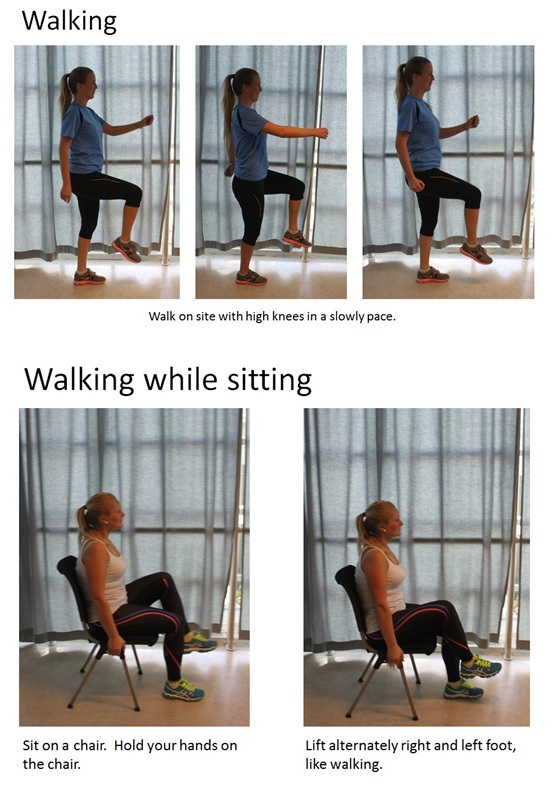
\includegraphics[scale=0.7]{Walking.jpg}
\label{app:walking}
\end{figure} 

\begin{figure} [H]
\centering
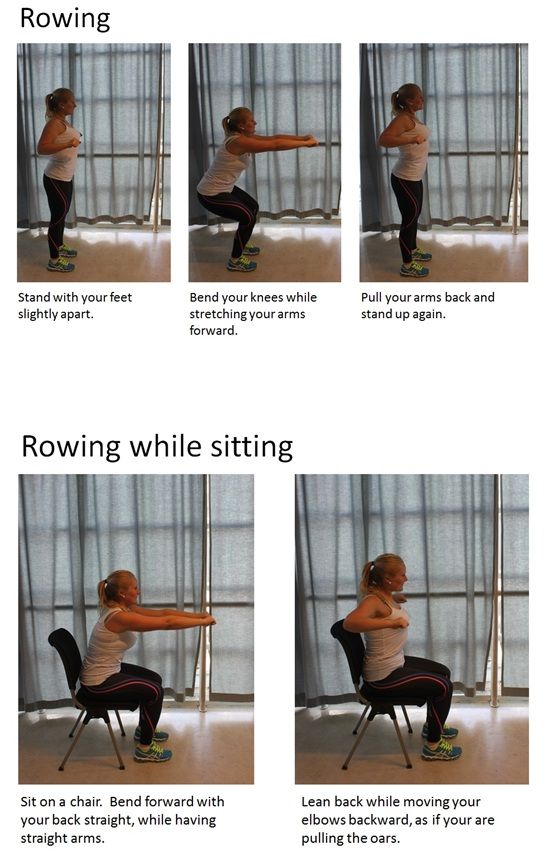
\includegraphics[scale=0.7]{Rowing.jpg}
\label{app:rowing}
\end{figure}

\begin{figure} [H]
\centering
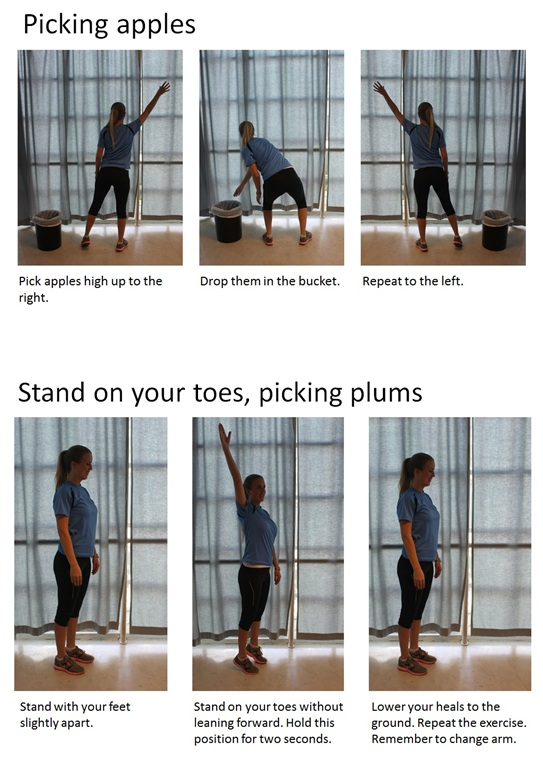
\includegraphics[scale=0.7]{PickingApples.jpg}
\label{app:pickingapplesApp}
\end{figure}

\begin{figure} [H]
\centering
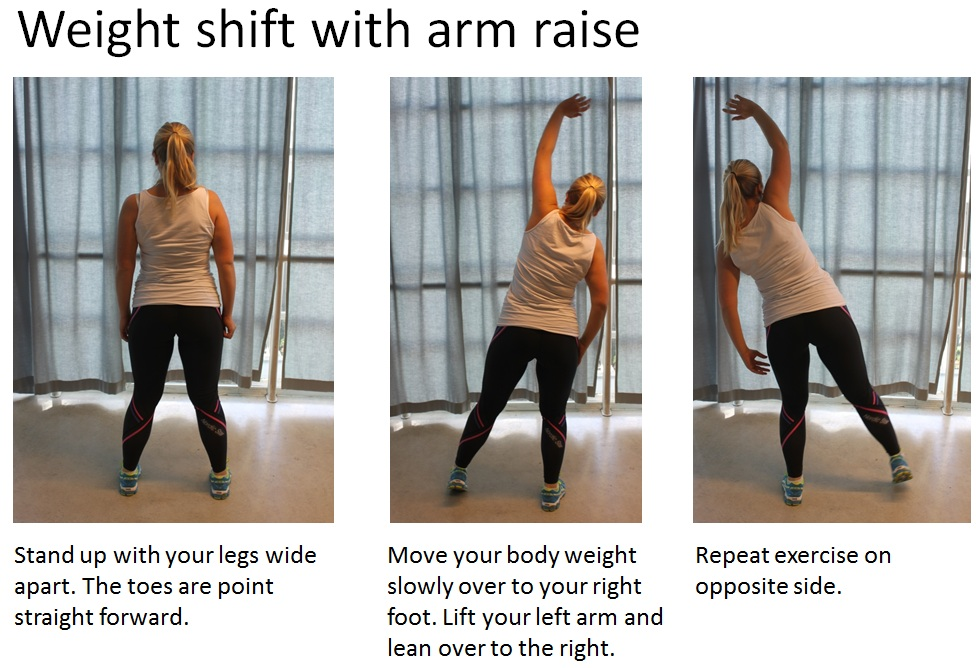
\includegraphics[scale=0.8]{WeightShift.jpg}
\label{app:weightshift}
\end{figure} 

\begin{figure} [H]
\centering
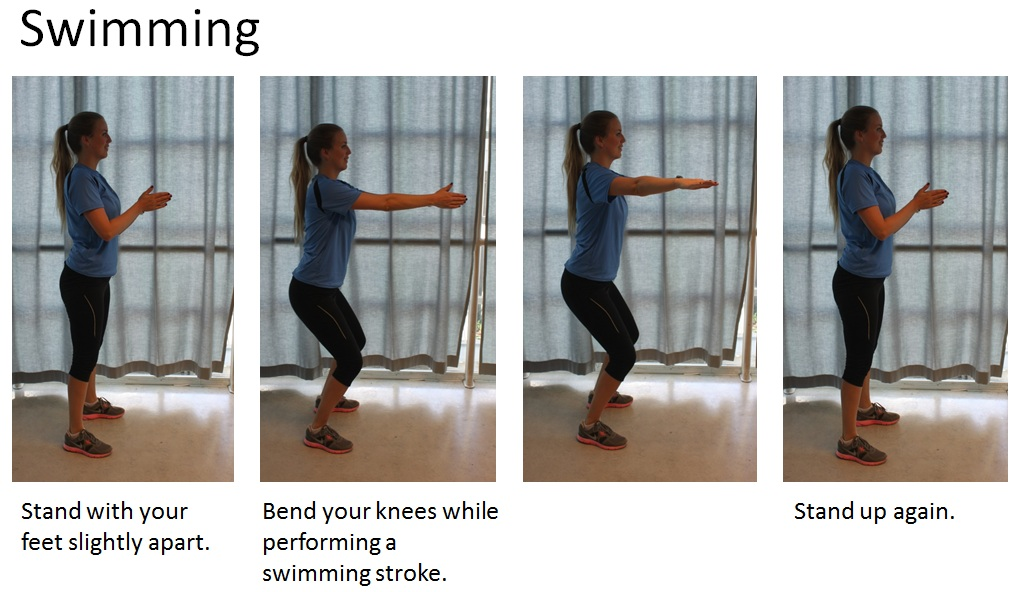
\includegraphics[scale=0.8]{Swimming.jpg}
\label{app:swimming}
\end{figure}

\begin{figure} [H]
\centering
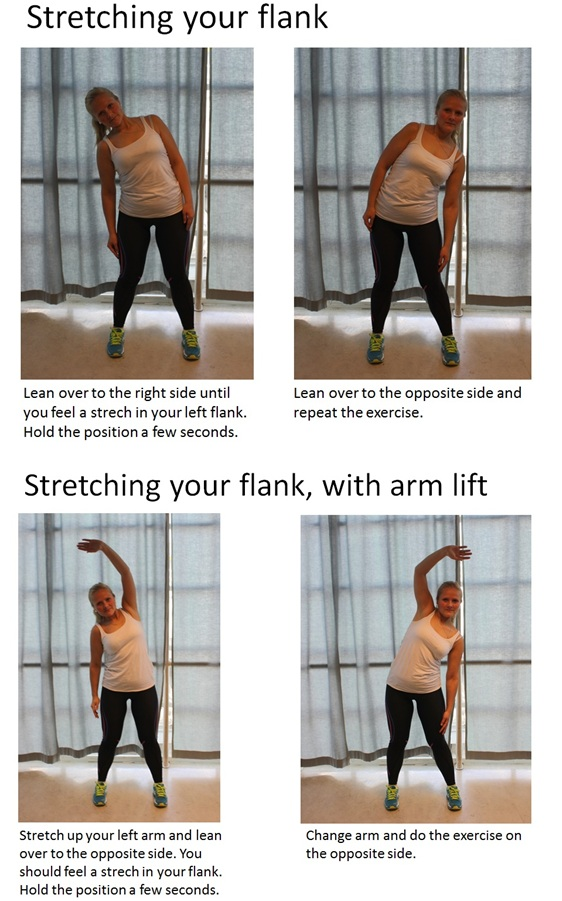
\includegraphics[scale=0.8]{StrechFlank.jpg}
\label{app:stretchflank}
\end{figure} 

\begin{figure} [H]
\centering
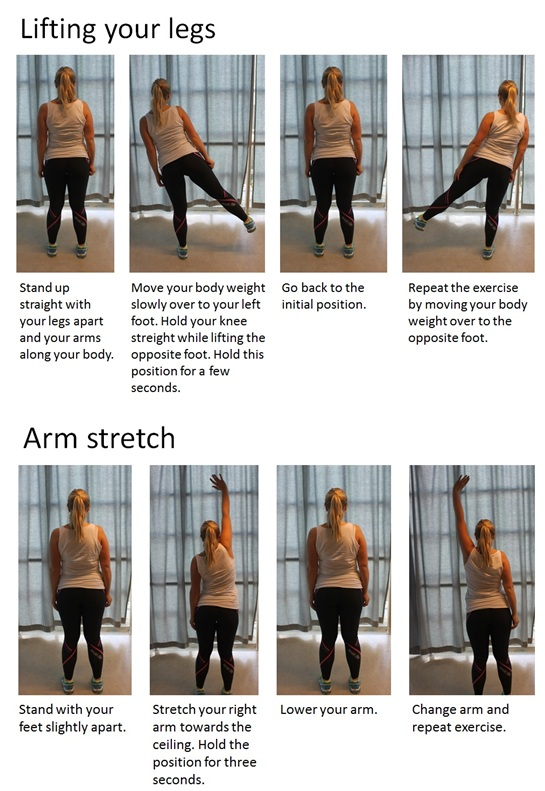
\includegraphics[scale=0.8]{LiftingYourLegs.jpg}
\label{app:liftlegs}
\end{figure} 


\begin{figure} [H]
\centering
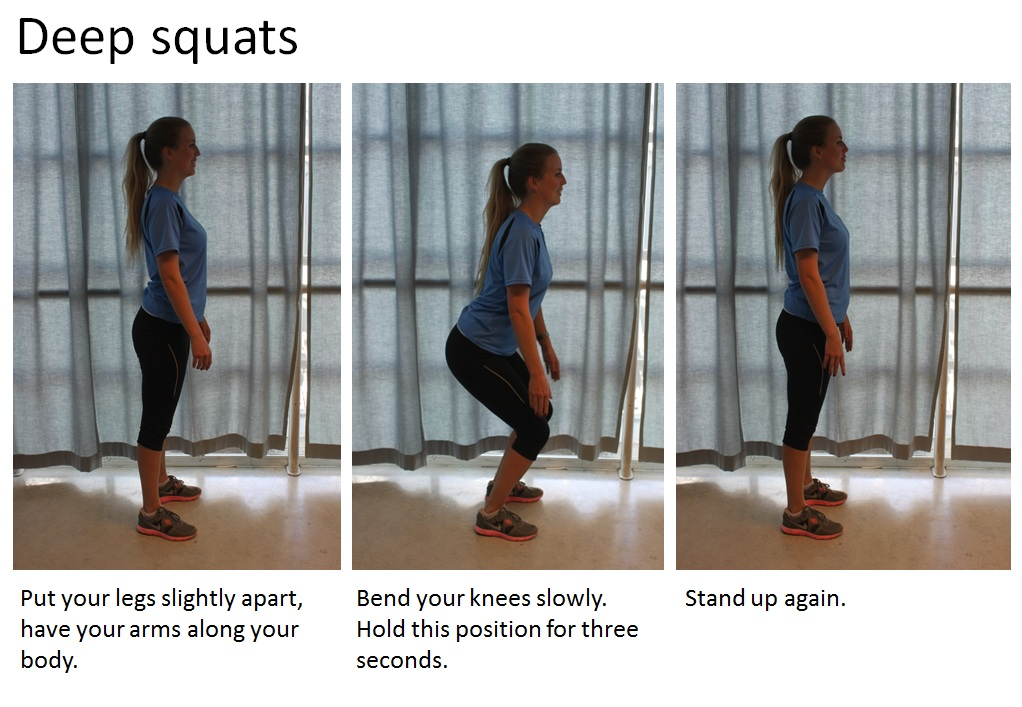
\includegraphics[scale=0.8]{Squats.jpg}
\label{app:squats}
\end{figure}  

\begin{figure} [H]
\centering
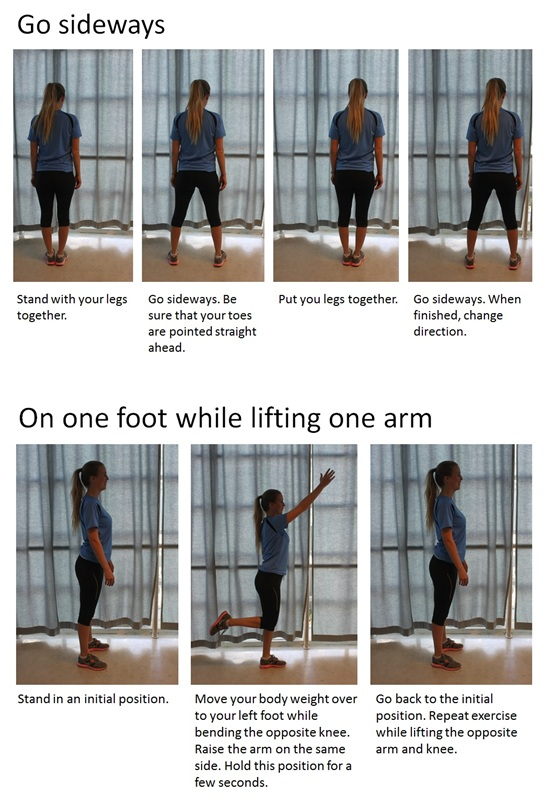
\includegraphics[scale=0.8]{GoSideways.jpg}
\label{app:gosideways}
\end{figure} 

\newpage
\section*{Appendix C - Various Steps from the Original Norwegian Exergame Concept}
\label{app:concept}

\begin{figure} [H]
\centering
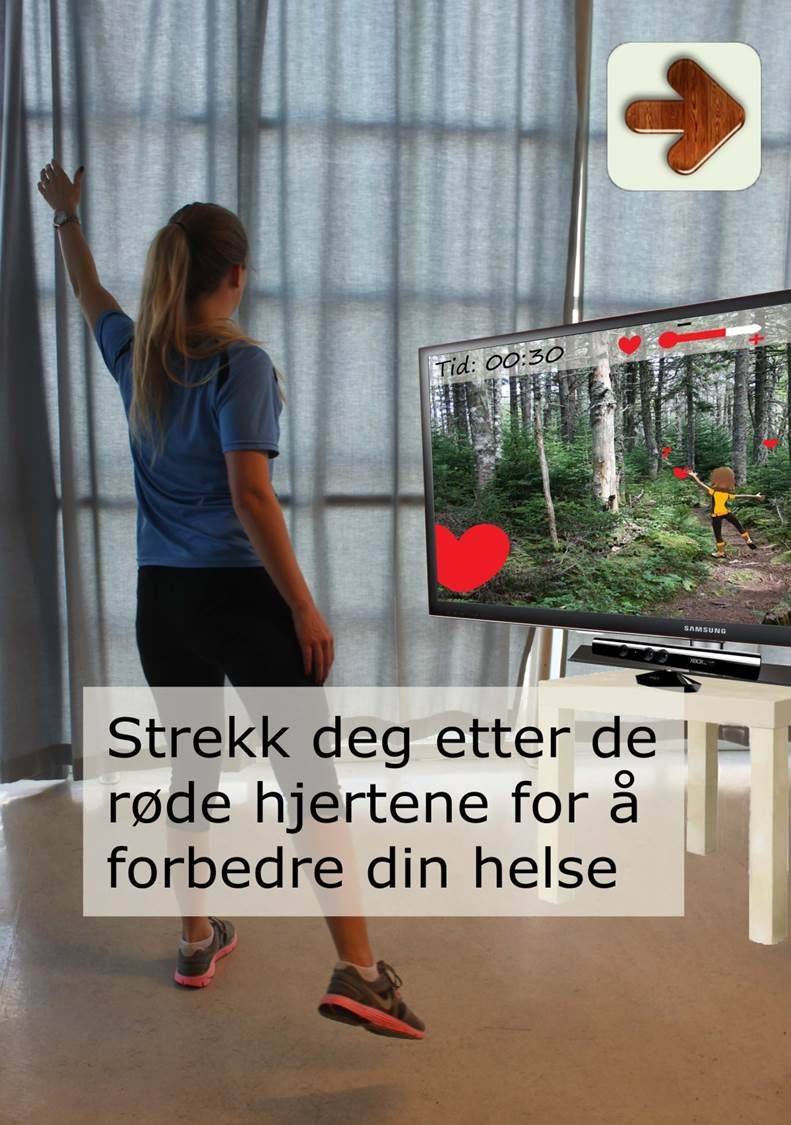
\includegraphics[scale=0.7]{KineIntro.jpg}
\label{fig:kineintroNorsk}
\end{figure}

\begin{figure} [H]
\centering
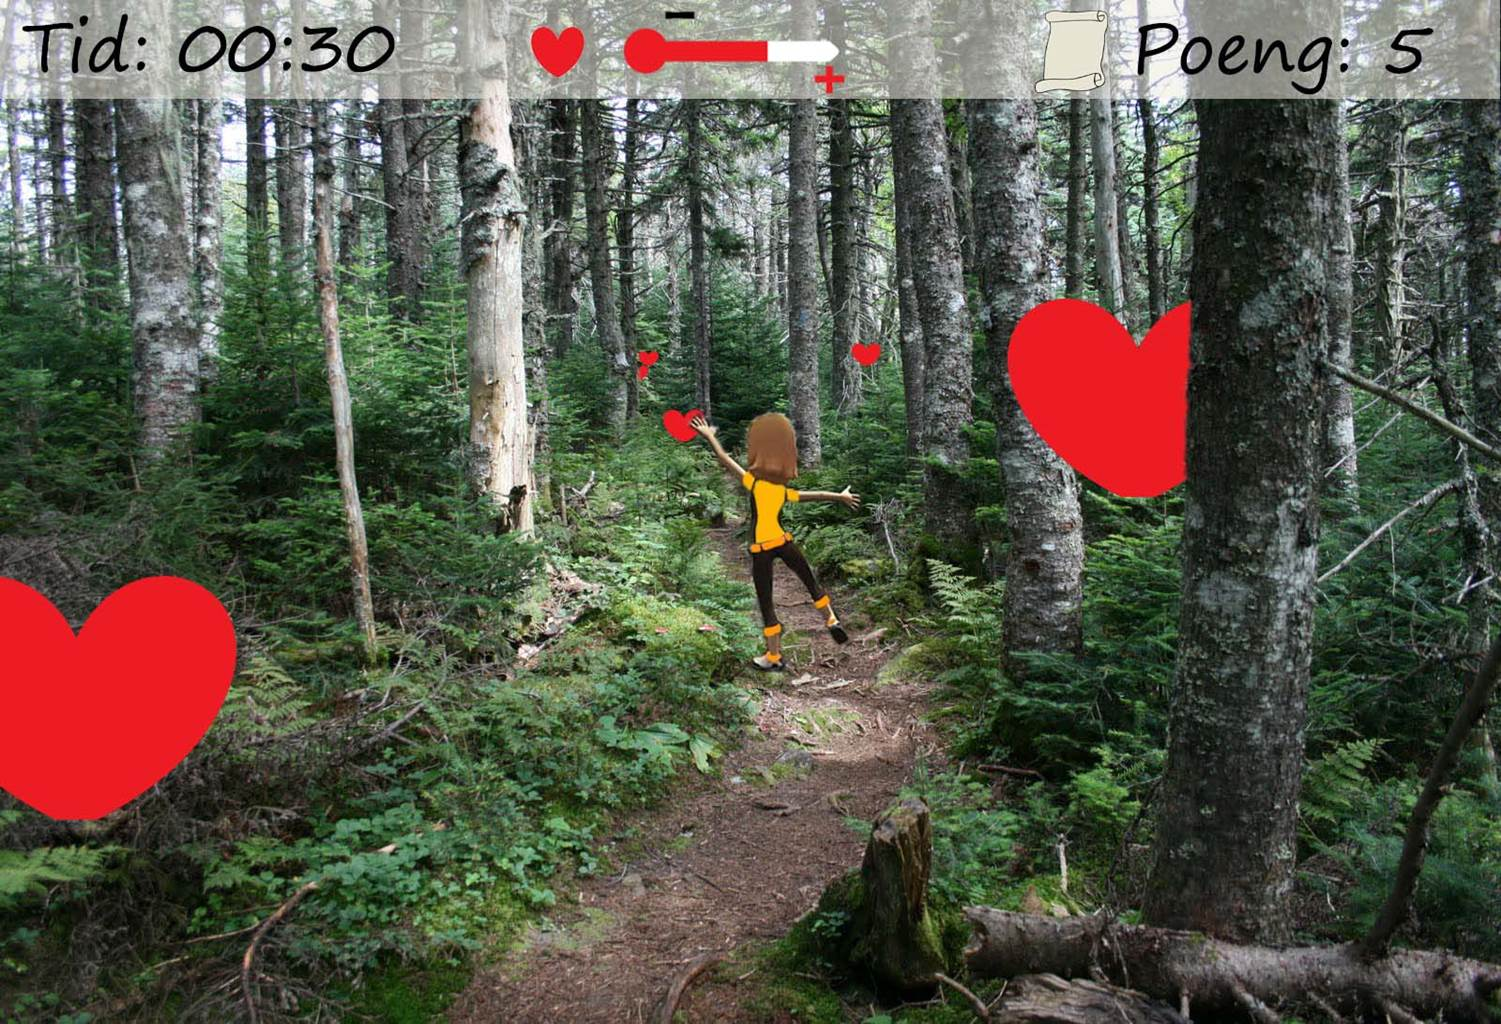
\includegraphics[scale=0.5]{hjerter.jpg}
\label{fig:heartsNorsk}
\end{figure}

\begin{figure} [H]
\centering
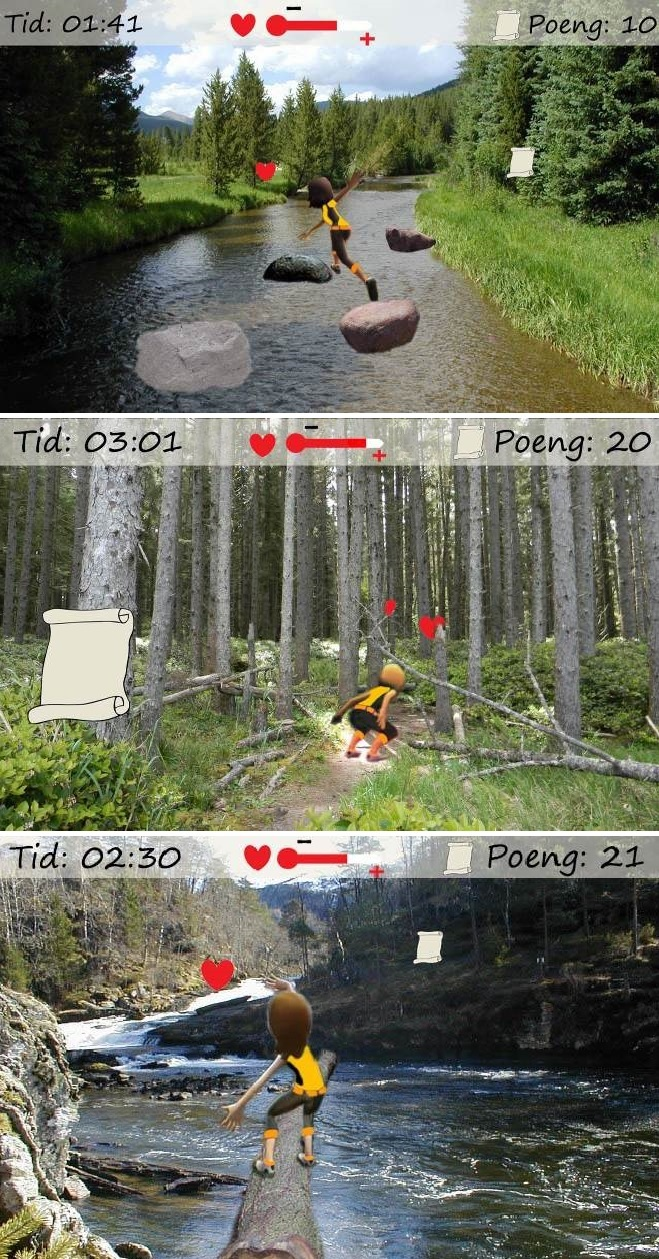
\includegraphics[scale=0.45]{hindring1.jpg}
\label{fig:hindring1Norsk}
\end{figure}

\begin{figure} [H]
\centering
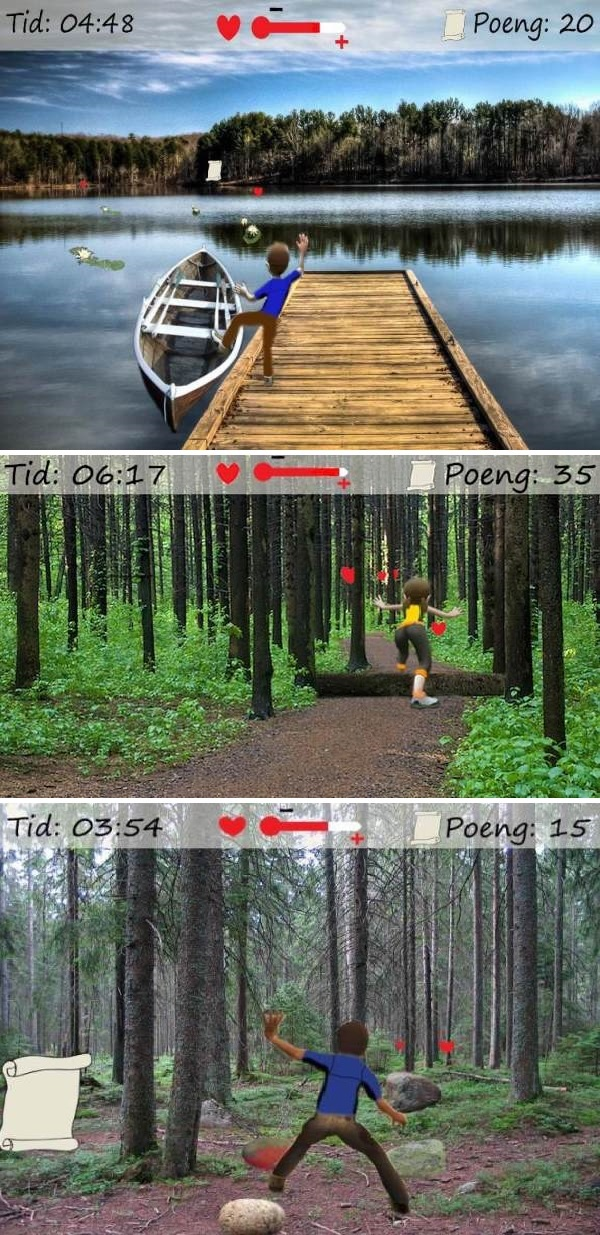
\includegraphics[scale=0.45]{hindring2.jpg}
\label{fig:hindring2Norsk}
\end{figure}

\begin{figure} [H]
\centering
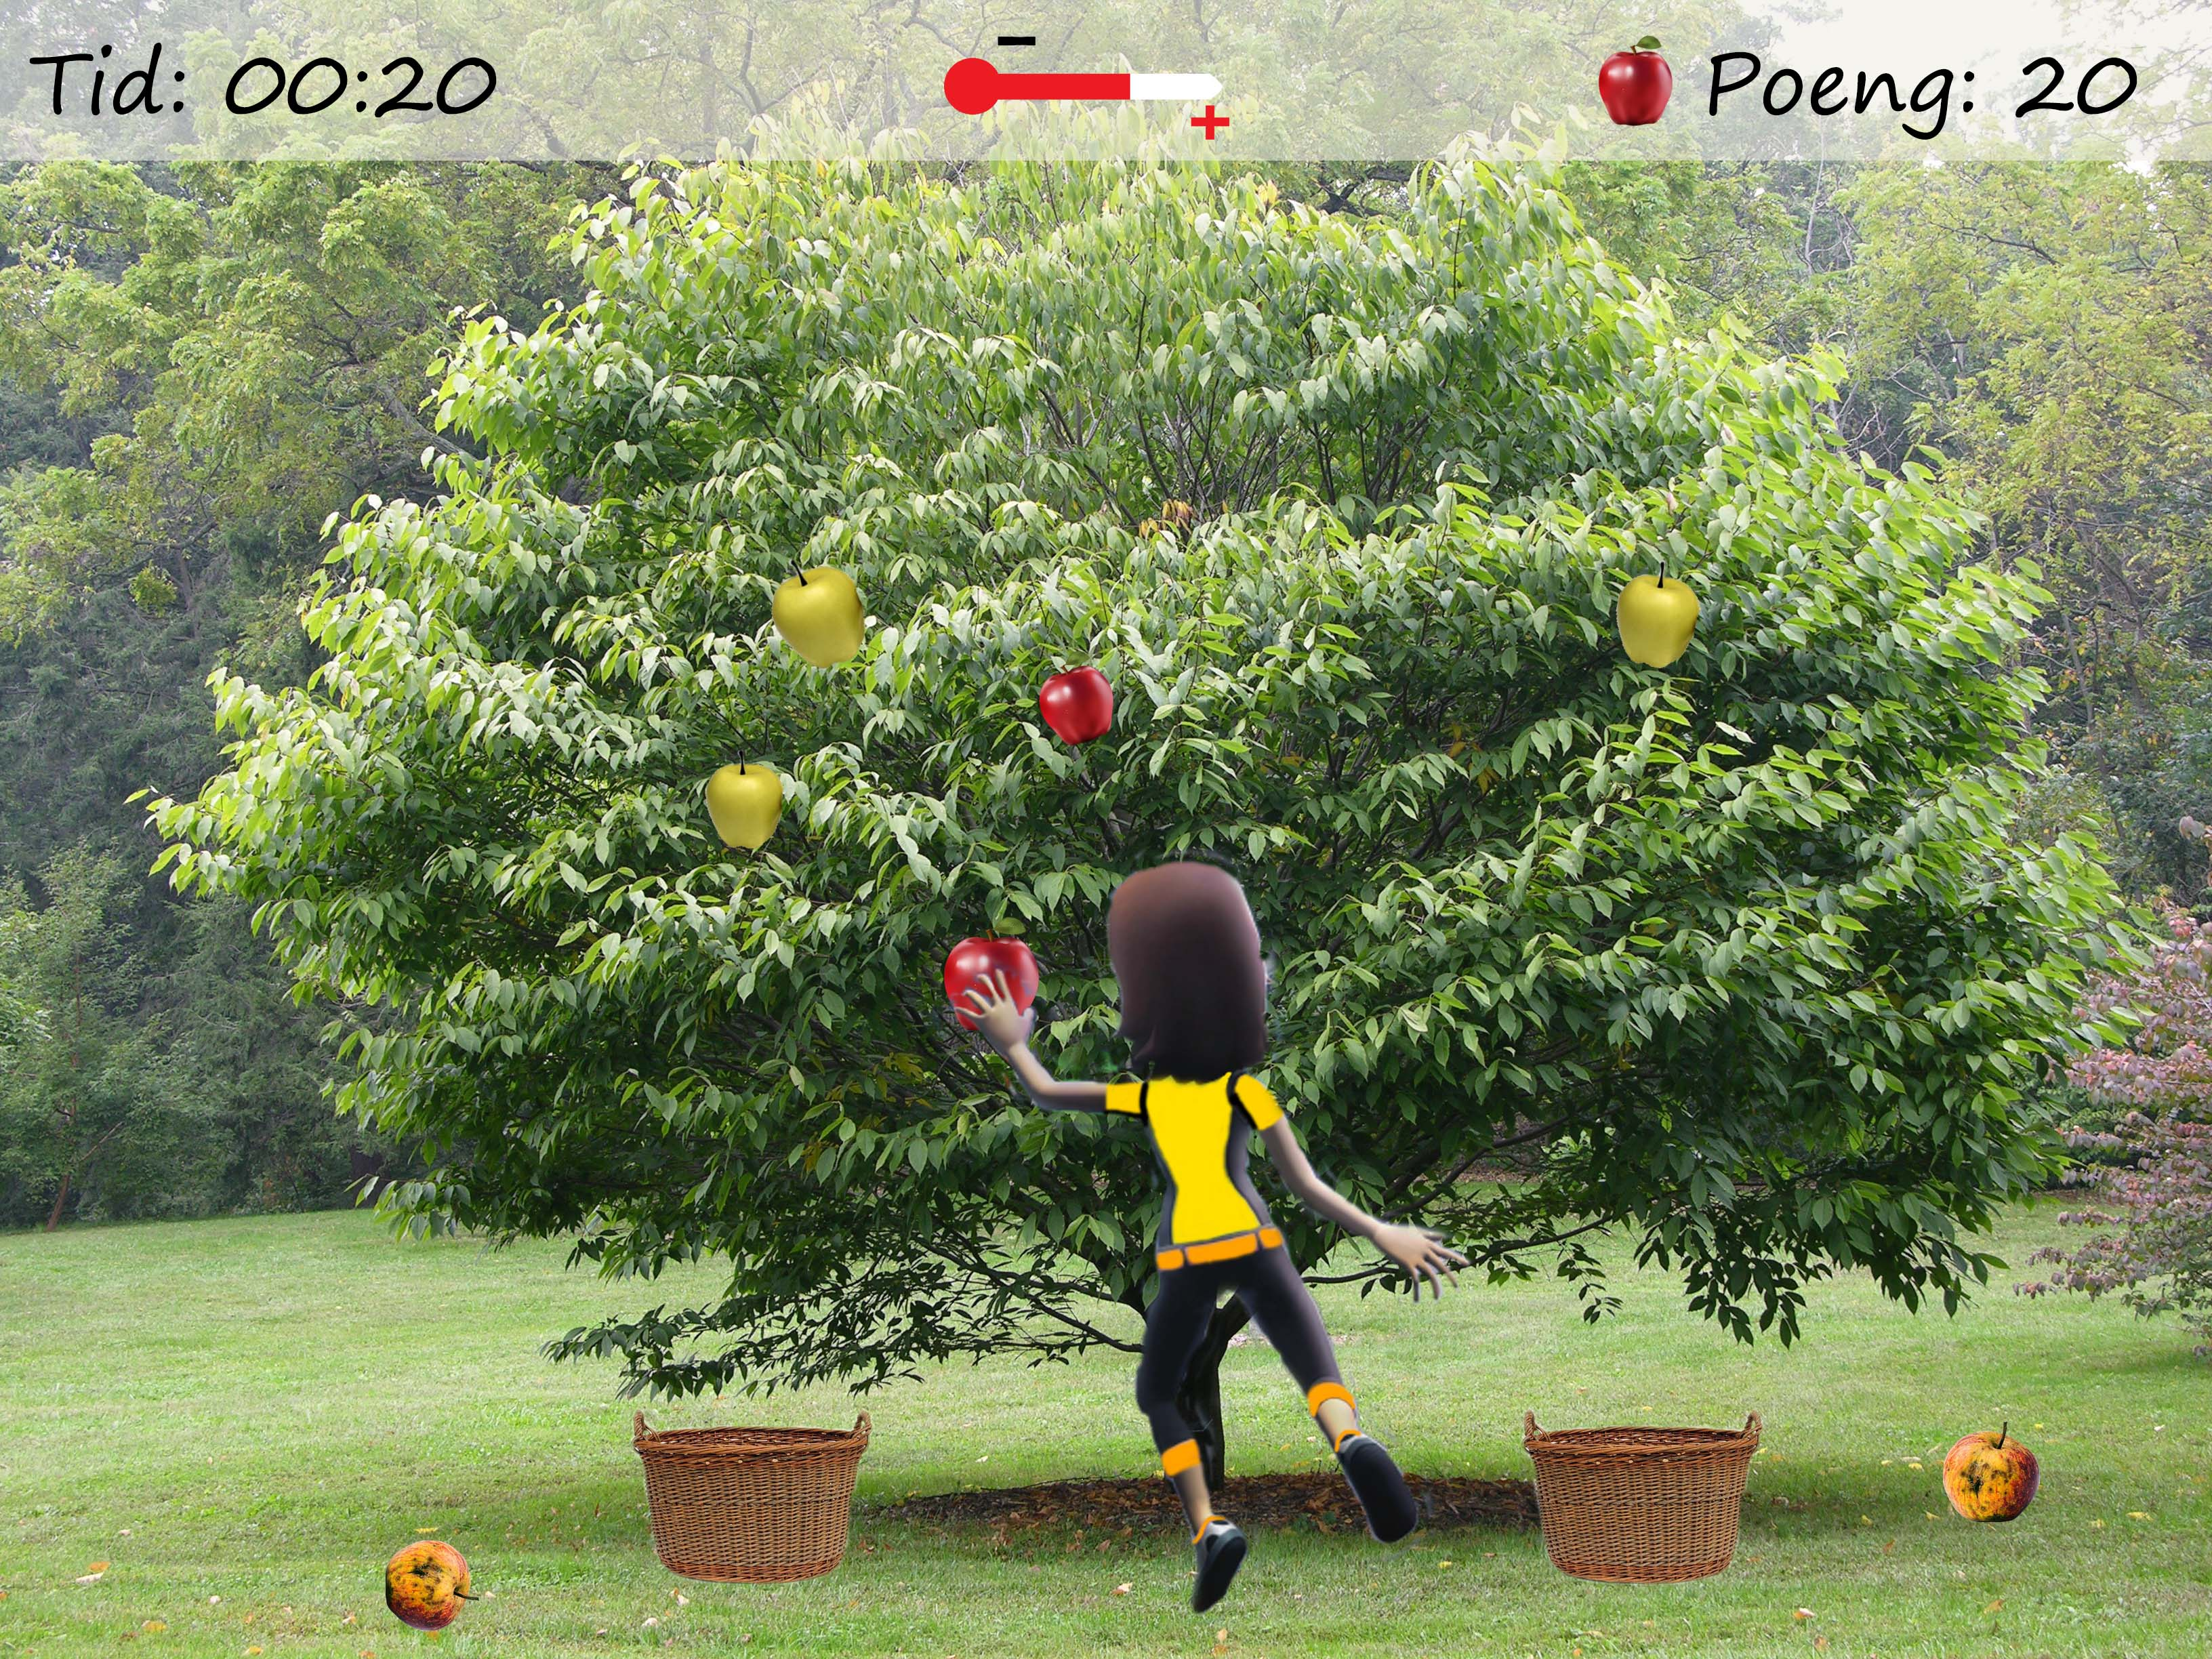
\includegraphics[scale=0.1]{gameappletree.jpg}
\label{fig:appleStretchNorsk}
\end{figure}

\begin{figure} [H]
\centering
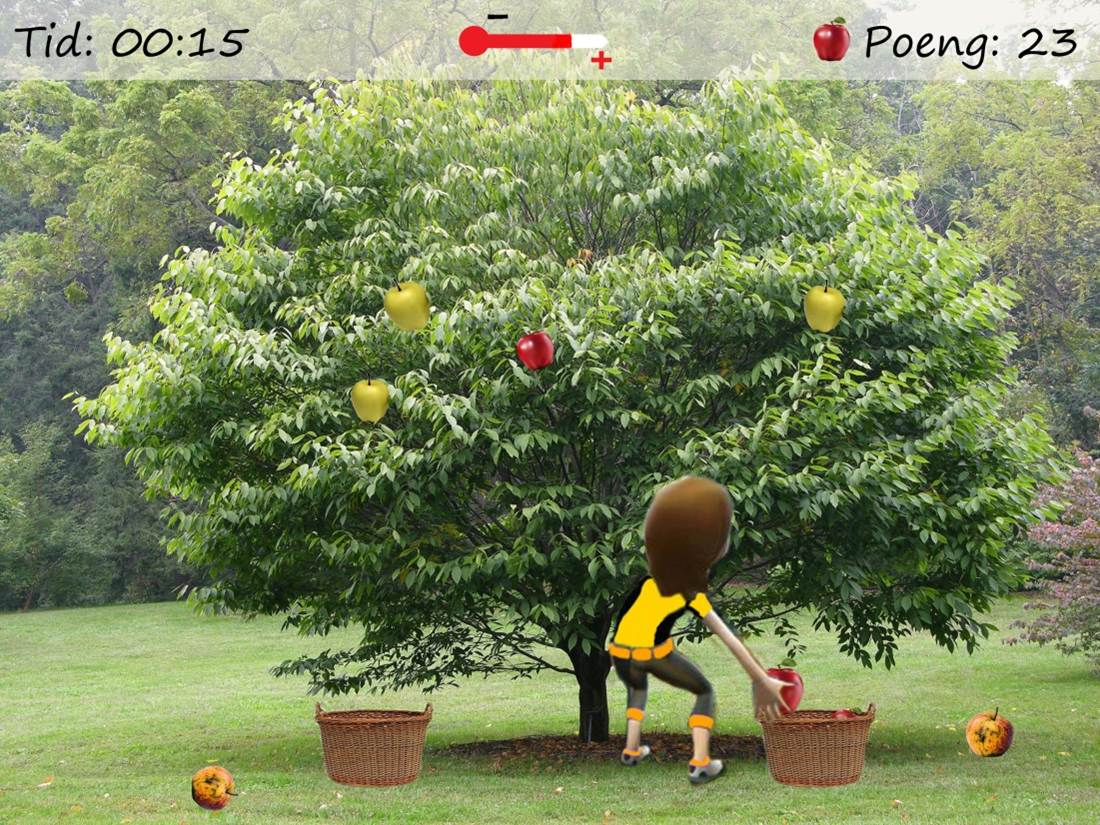
\includegraphics[scale=0.45]{squateple.jpg}
\label{fig:appleSquatNorsk}
\end{figure}

\begin{figure} [H]
\centering
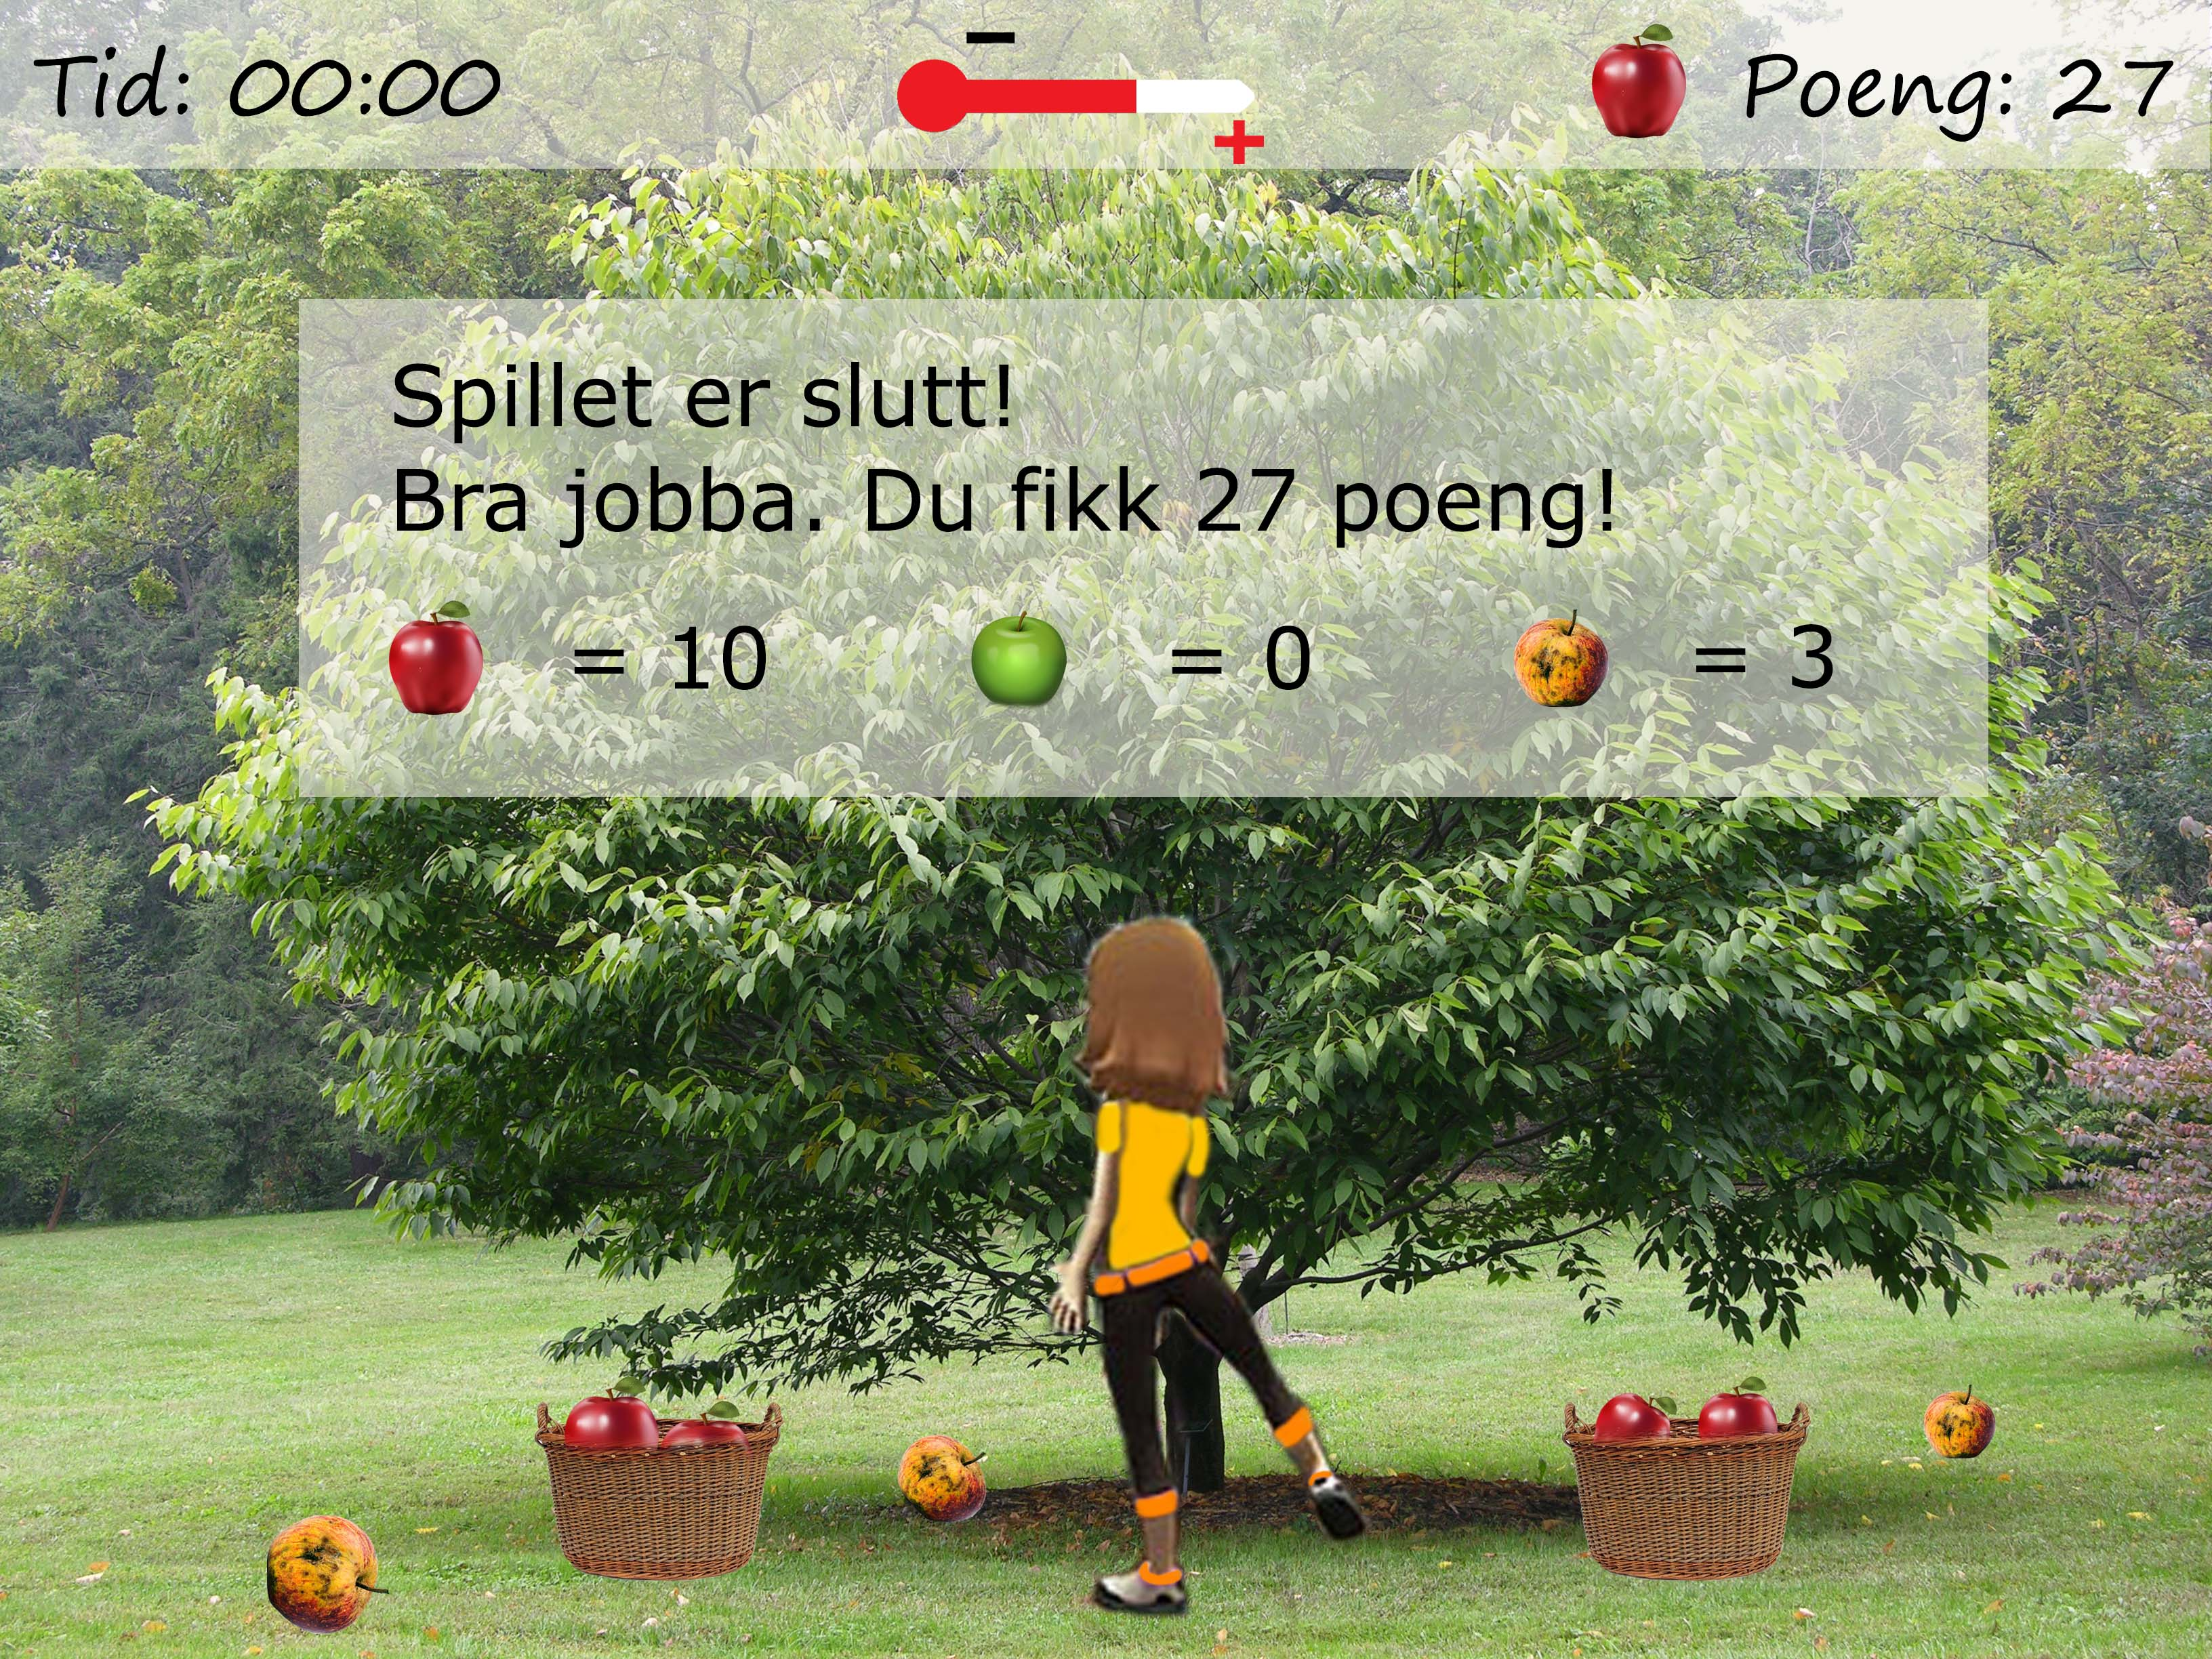
\includegraphics[scale=0.1]{appletreeend.jpg}
\label{fig:appleOverNorsk}
\end{figure}

\begin{figure} [H]
\centering
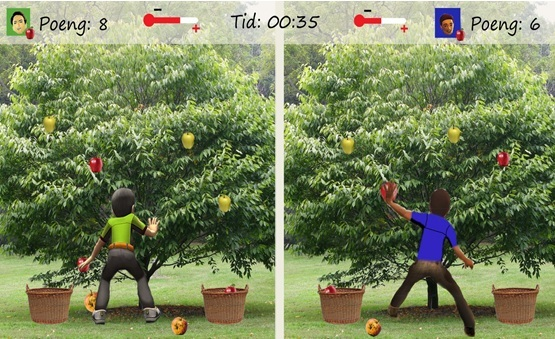
\includegraphics[scale=0.8]{multiplayereple.jpg}
\label{fig:appleMultiplayerNorsk}
\end{figure}

\begin{figure} [H]
\centering
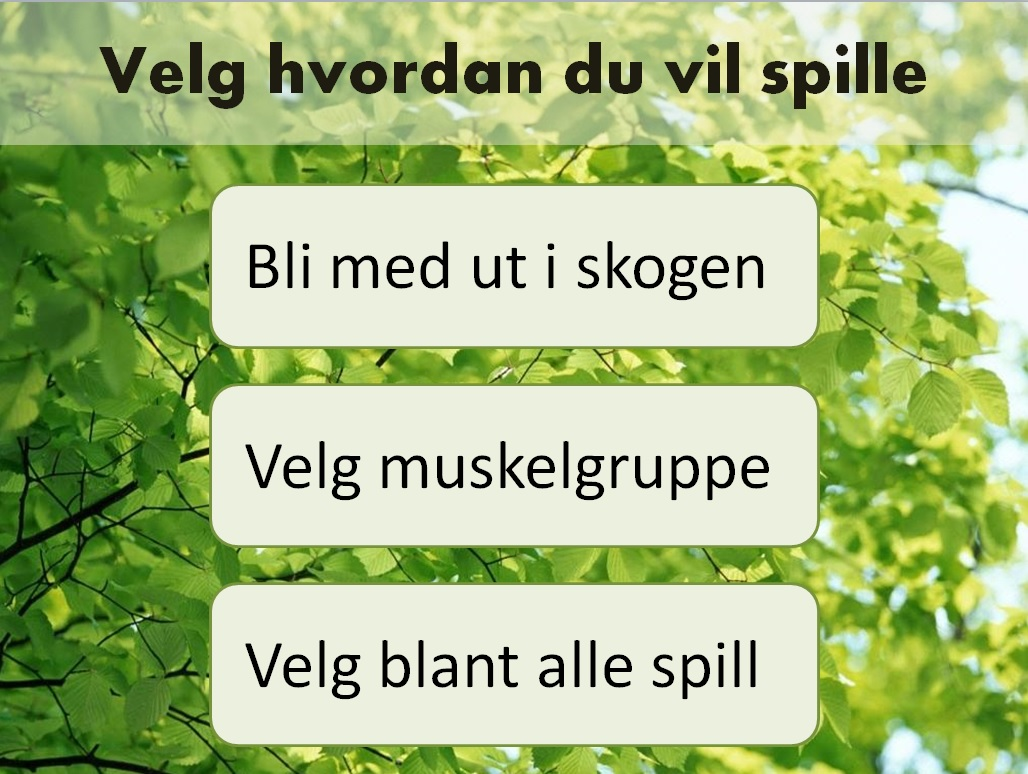
\includegraphics[scale=0.45]{menuStart.jpg}
\label{fig:menuStartNorsk}
\end{figure} 

\begin{figure} [H]
\centering
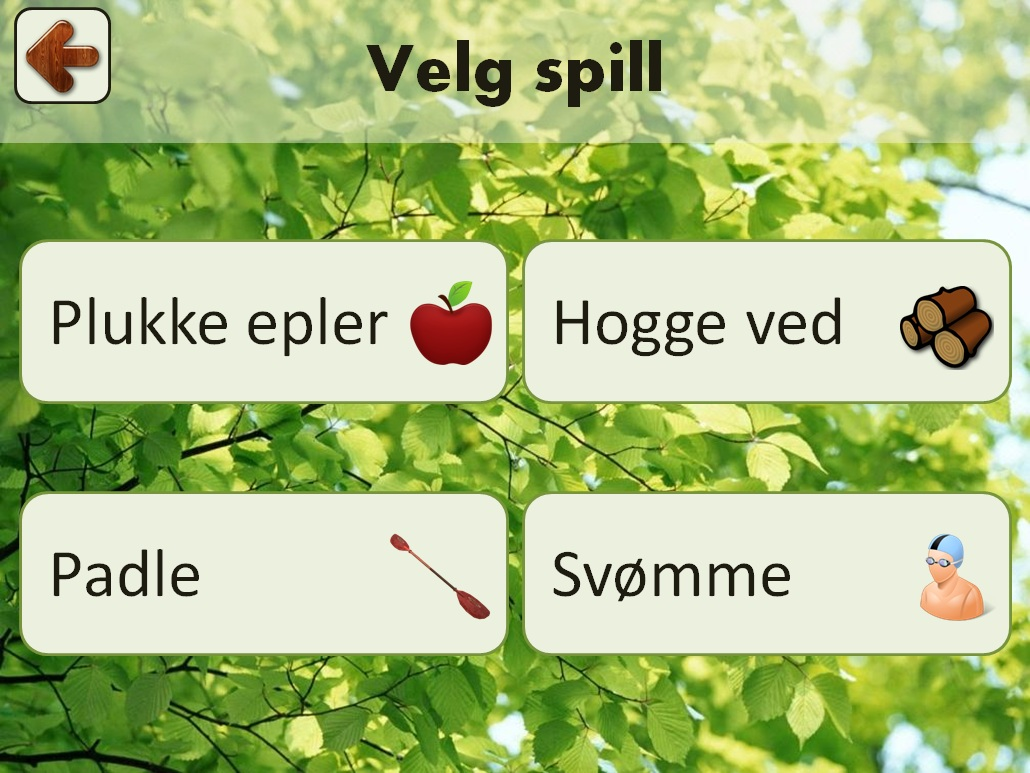
\includegraphics[scale=0.4]{VelgSpill.jpg}
\label{velgSpillNorsk}
\end{figure}

\begin{figure} [H]
\centering
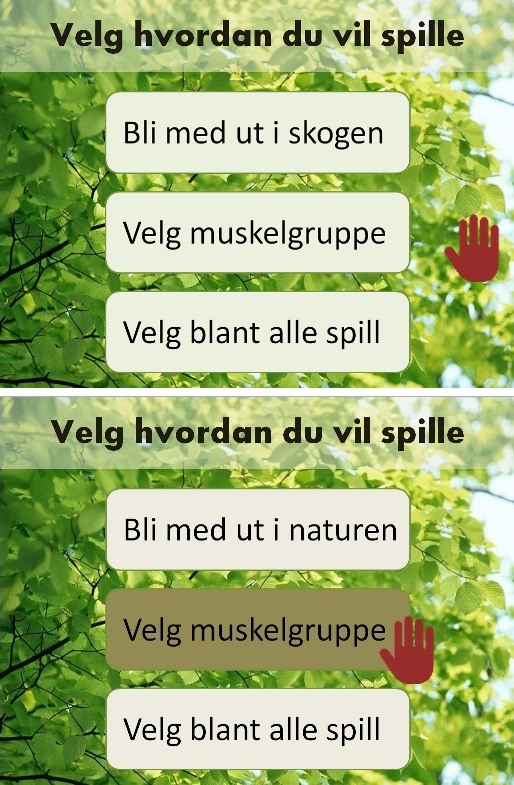
\includegraphics[scale=0.5]{menuAvatarAction.jpg}
\label{fig:avatarActionNorsk}
\end{figure} 

\begin{figure} [H]
\centering
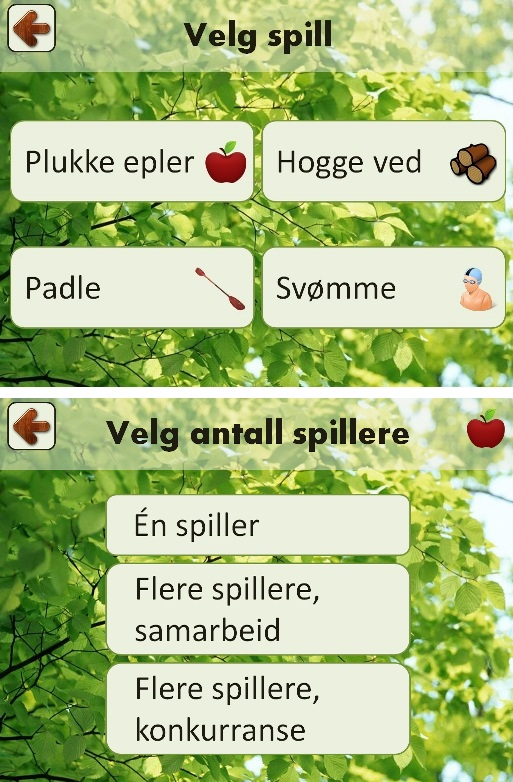
\includegraphics[scale=0.5]{IconEple.jpg}
\label{fig:iconEpleNorsk}
\end{figure} 

\begin{figure} [H]
\centering
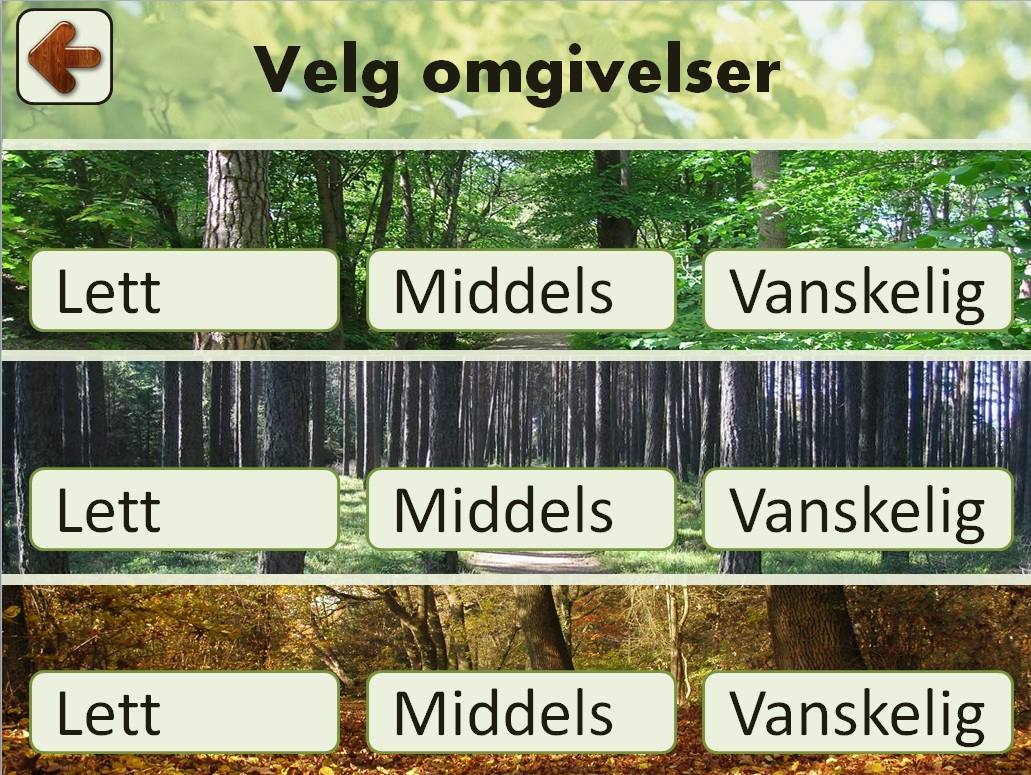
\includegraphics[scale=0.45]{VelgOmgivelser.jpg}
\label{fig:omgivelseNivaaNorsk}
\end{figure}

\begin{figure} [H]
\centering
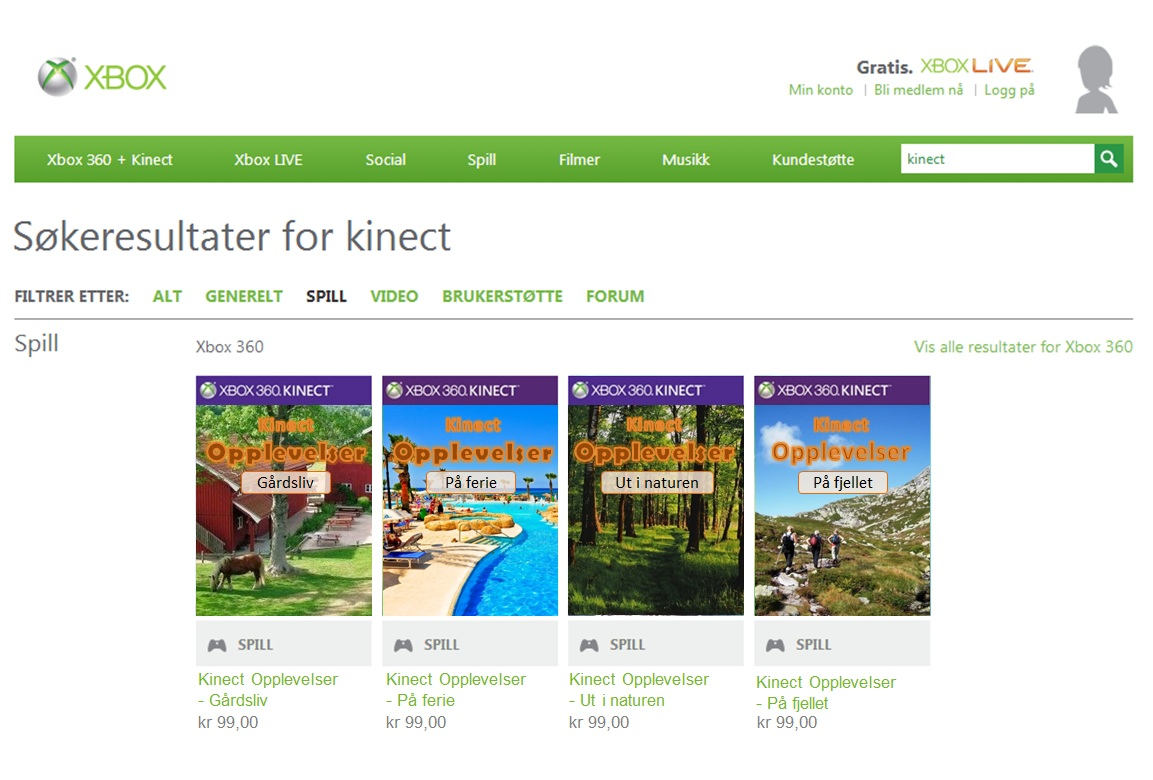
\includegraphics[scale=0.5, angle=90]{SpillXboxNYNY.jpg}
\label{fig:videogameseriesHeleNorsk}
\end{figure}

\newpage
\section*{Appendix D - Review of the Original Norwegian Menu}
\label{app:menureview}

The figures shown in Appendix C shows a review of the original prototypes of the menu. This menu was presented for the informants in workshop 2, and is therefore in Norwegian. The menu review starts with the choice on how to play. The player chooses to play according to a preferred muscle group. A selection of single games are shown, where the player chooses "picking apples". The menu shows a start, middle, and end scene from this game. When finished, the player chooses to change number of players from single player to multi player.  

\begin{figure} [H]
\centering
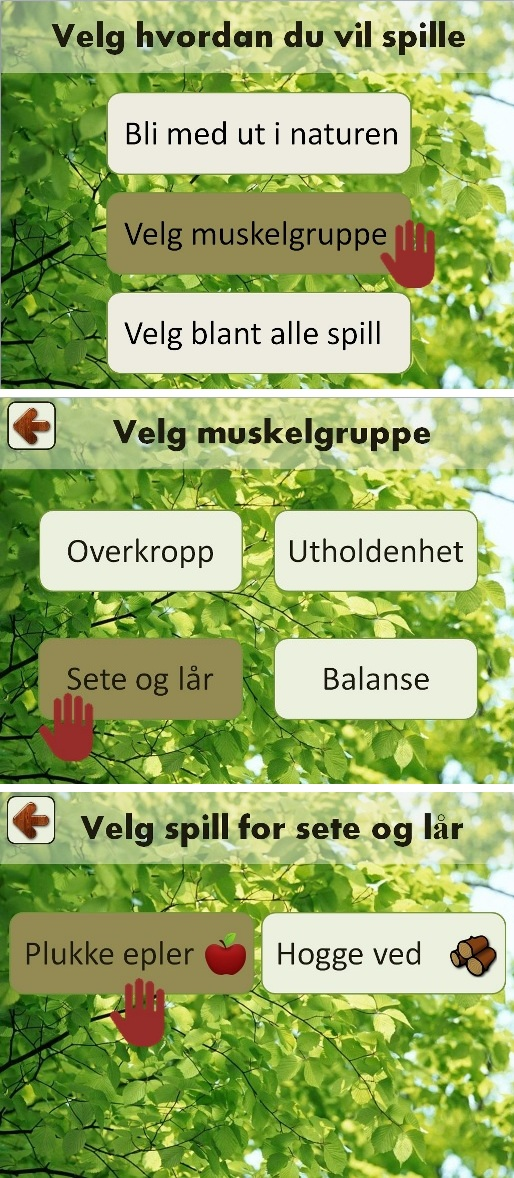
\includegraphics[scale=0.45]{menuStep1.jpg}
\label{app:menu1Norsk}
\end{figure}

\begin{figure} [H]
\centering
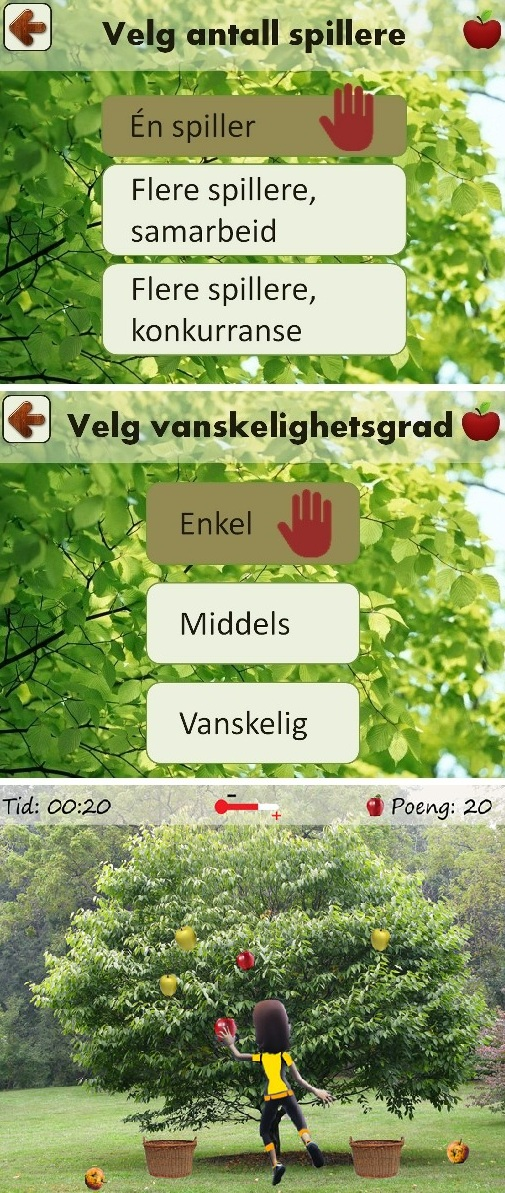
\includegraphics[scale=0.45]{menuStep2.jpg}
\label{app:menu2Norsk}
\end{figure}

\begin{figure} [H]
\centering
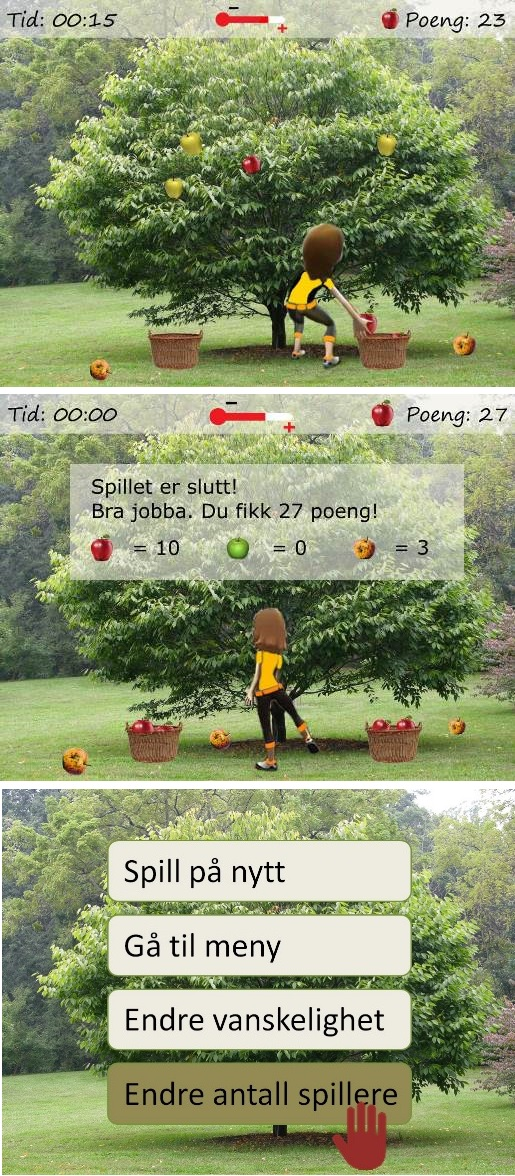
\includegraphics[scale=0.45]{menuStep3.jpg}
\label{app:menu3Norsk}
\end{figure}

\begin{figure} [H]
\centering
\includegraphics[scale=0.45]{menuStep4.jpg}
\label{app:menu4Norsk}
\end{figure}

\newpage
\section*{Appendix E - Response on our Application to NSD}
\label{app:presentation}
\begin{figure}[H] 
\centering{\includegraphics[scale=0.6]{NSD1.pdf}}
\end{figure}  
\begin{figure}[H] 
\centering{\includegraphics[scale=0.6]{NSD2.pdf}}
\end{figure} 

\newpage
\section*{Appendix F - Informed Consent}
\label{app:infoConsent}
\begin{figure}[H] 
\centering{\includegraphics[scale=0.65]{Info-samtykke-til-senior1.pdf}}
\end{figure}  
\begin{figure}[H] 
\centering{\includegraphics[scale=0.65]{Info-samtykke-til-senior2.pdf}}
\end{figure} 

\newpage
\section*{Appendix G - Questionnaire}
\label{app:questionnaire}
\begin{figure}[H] 
\centering{\includegraphics[scale=0.65]{SU1.pdf}}
\end{figure}  
\begin{figure}[H] 
\centering{\includegraphics[scale=0.65]{SU2.pdf}}
\end{figure}  
\begin{figure}[H] 
\centering{\includegraphics[scale=0.65]{SU3.pdf}}
\end{figure}  
\begin{figure}[H] 
\centering{\includegraphics[scale=0.65]{SU4.pdf}}
\end{figure}  
\begin{figure}[H] 
\centering{\includegraphics[scale=0.65]{SU5.pdf}}
\end{figure}  
\begin{figure}[H] 
\centering{\includegraphics[scale=0.65]{SU6.pdf}}
\end{figure}  

\newpage
\section*{Appendix H - Interview Guide for the Focus Group Interview}
\label{app:interviewGuide}
\begin{figure}[H] 
\centering{\includegraphics[scale=0.65]{questions.pdf}}
\end{figure}  
  
\addcontentsline{toc}{chapter}{Appendix}
\cleardoublepage
\end{document}

